% !TEX options=--shell-escape
\documentclass[usenames,dvipsnames,9pt]{beamer}
\usetheme{metropolis}

% Not working in Overleaf
% \makeatletter
% \def\input@path{{../support/beamer-template/}}
% \makeatother
% \usepackage{../support/beamer-template/beamerthememetropolis}

\usepackage[utf8]{inputenc}
\usepackage[czech]{babel}
\selectlanguage{czech}

\usepackage{hyperref}
\usepackage{fontawesome}
\usepackage{minted}
\usepackage{mathtools}
\usepackage{tabularx}
\usepackage{smartdiagram}
\usepackage{soul}
\usepackage{tikz}
\usepackage{amssymb}
\usepackage{qrcode}

% Commands shared between most of the tutorial slides

% Homework deadlines
\newcommand{\hwVIIdeadline}{10. 5. 2020}



% Download icon and text with link relative to the root of the courseware site
\newcommand{\download}[1]{\hfill\faDownload\hspace{5pt}\href{https://cw.fel.cvut.cz/wiki/_media/courses/be4m36mas/#1}{\tt #1}\\[1.3em]}

% Draw eye icon
\newcommand{\see}[1]{\faEye\hspace{5pt}#1}

\newcommand{\sep}{\hspace{10pt}/\hspace{10pt}}

\def\Ipe#1{\def\IPEfile{#1}\input{#1}}

% Draw pacman icon
\newcommand{\pacman}[1]{\tikz[baseline=.1em,scale=.6]{
    \useasboundingbox (.02,0) rectangle (.6,.6);
  \draw [fill=#1] (.3,.3) -- ++(25:.3) arc (+25:+335:.3) -- cycle;

}}

% Draw ghost icon
\newcommand{\ghost}[1]{\tikz[baseline=.1em,scale=.5]{
  \draw [fill=#1] (0,0) -- (0,.5) arc (+180:0:.3) -- (.6,0) --
  (.5,.15) -- (.4,0) -- (.3,.15) -- (.2,0) -- (.1,.15) -- cycle;
    \coordinate (eye) at (360*rand:.03);
    \foreach \x in {.17,.43}{
      \fill[white] (\x,.5) circle[radius=.1];
      \fill[black] (\x,.5) ++(eye) circle[radius=.05];
    }
}}

\newcommand{\desc}[2]{
  #1

  \vspace{-0.6em}
  \hfill\begin{minipage}{0.9\linewidth}
    #2
  \end{minipage}

  \vspace{0.2em}
}

\newcommand{\redc}{\tikz\draw[red,fill=red] (0,0) circle (.5ex);}

\newcommand{\greenc}{\tikz\draw[green,fill=green] (0,0) circle (.5ex);}


% Default url for generating QR code with feedback form.
\newcommand{\defaultfeedbackurl}{https://forms.gle/vwbWazEu14w1Kf487}

% Generate frame with QR code to a feedback form.
\newcommand{\framefeedback}[1][\defaultfeedbackurl]{
  \begin{frame}[standout]
    \begin{minipage}{0.4\linewidth}
      \begin{center}
        \textbf{\LARGE Díky za pozornost!}
      \end{center}

      \vspace{3em}

      \raggedleft\small Budeme rádi za Vaši\\zpětnou vazbu! $\rightarrow$
    \end{minipage}
    \hfill
    \begin{minipage}{0.5\linewidth}
      \vspace{4em}
      \centering\qrcode[height=\linewidth]{#1}\\
      \vspace{0.8em}
      \url{#1}
    \end{minipage}
  \end{frame}
}

\title{Paralelní maticové operace}
\date{\today}
\institute{B4B36PDV -- Paralelní a distribuované výpočty}

\metroset{block=fill}

\begin{document}
\maketitle

\begin{frame}
  \frametitle{Osnova}
  \begin{itemize}
    %\item Opakování z minulého cvičení\\[1.5em]
    \item Paralelní maticové operace
    \item Semestrální úloha\\[1.5em]
    %\item Zadání semestrální úlohy
  \end{itemize}
\end{frame}


%\section{Opakování z minulého cvičení}
%
%\begin{frame}[standout]
%  \Huge
%  \url{http://goo.gl/a6BEMb}
%\end{frame}
%
%{\setbeamertemplate{frame footer}{\see{\url{http://goo.gl/a6BEMb}}}
%\begin{frame}[fragile]
%\frametitle{Který způsob je efektivnější?}
%
% \begin{minted}{c}
%bool mat[M][N];
% \end{minted}
%
%\end{frame}
%
%\begin{frame}[fragile]
%\frametitle{Jakým způsobem bude následující kód proveden?}
%
% \begin{minted}{c}
%std::cout << "Finished!" << std::endl;
% \end{minted}
% 
% \vspace{.3em}
% 
% \begin{itemize}
% \item MOZNOST A
% \end{itemize}
%
%\end{frame}
%}

\section{Paralelní maticové operace}

\begin{frame}
  \frametitle{Násobení vektorů}
  
  Skalární součin vektorů $u$ a $v$ délky $n$ lze spočítat jako
  
  \begin{equation*}
  u\times v = \sum_{i=0}^{n-1} u[i]\cdot v[i]
  \end{equation*}
  
  \vspace{1em}\hrule\vspace{1em}
  
  \begin{center}
  \Large Co když je mnoho prvků v obou vektorech nulových?
  \end{center}
  
    \pause\vspace{1em}

\faWarning\hspace{3pt} Potom je neefektivní jak samotné násobení, tak i vektorová reprezentace

\end{frame}

\begin{frame}
  \frametitle{Řídké vektory}
  
 Vektory s {\bf málo nenulovými hodnotami} lze reprezentovat kompaktněji!
 
 Místo toho, abychom si pamatovali všechny (i nulové) prvky, tak si pamatujeme pouze:
 \begin{itemize}
 \item na jakých indexech jsou nenulové prvky
 \item jaké hodnoty jsou na těchto indexech
 \end{itemize}
 
 \pause\vspace{1em}
 
 Např. vektor $v = (0,0,0,0,3,0,1,0,0,0,2)$ reprezentujeme pomocí
 $v = \lbrace (4,3),\ \ (6,1),\ \ (10,2) \rbrace$
 
   \vspace{1em}\pause\hrule\vspace{1em}
 
  Jak spočteme skalární součin vektorů $u$ a $v$?
  
  \begin{tabular}{ccccc}
    \only<3>{\redc} & \only<4>{\redc} & \only<5-6>{\redc} & \only<7-8>{\redc} & \\
    (1,1) & (2,5) & (6,2) & (8,2) & \\
    (2,3) & (4,3) & (6,1) & (4,2) & \\
    \only<3-4>{\greenc} & \only<5>{\greenc} & \only<6>{\greenc} & \only<7>{\greenc} & \only<8>{\greenc}
  \end{tabular}
  

\end{frame}

\begin{frame}
  \frametitle{Násobení matice vektorem}
  
  Součin matice A o rozměrech $m \times n$ a vektoru $u$ délky $n$ lze spočítat jako 
  
    \begin{equation*}
  Au = (A_1\times u, A_2 \times u, \dots, A_m \times u),
  \end{equation*}
  
  kde $A_i,~i\in [m]$ jsou jednotlivé řádky matice $A$.
  
   \pause\vspace{1em}
  
  \begin{center}
  \Large Jak tento výpočet zparalelizovat?
  \end{center}
  
  \pause
  
  \begin{center}
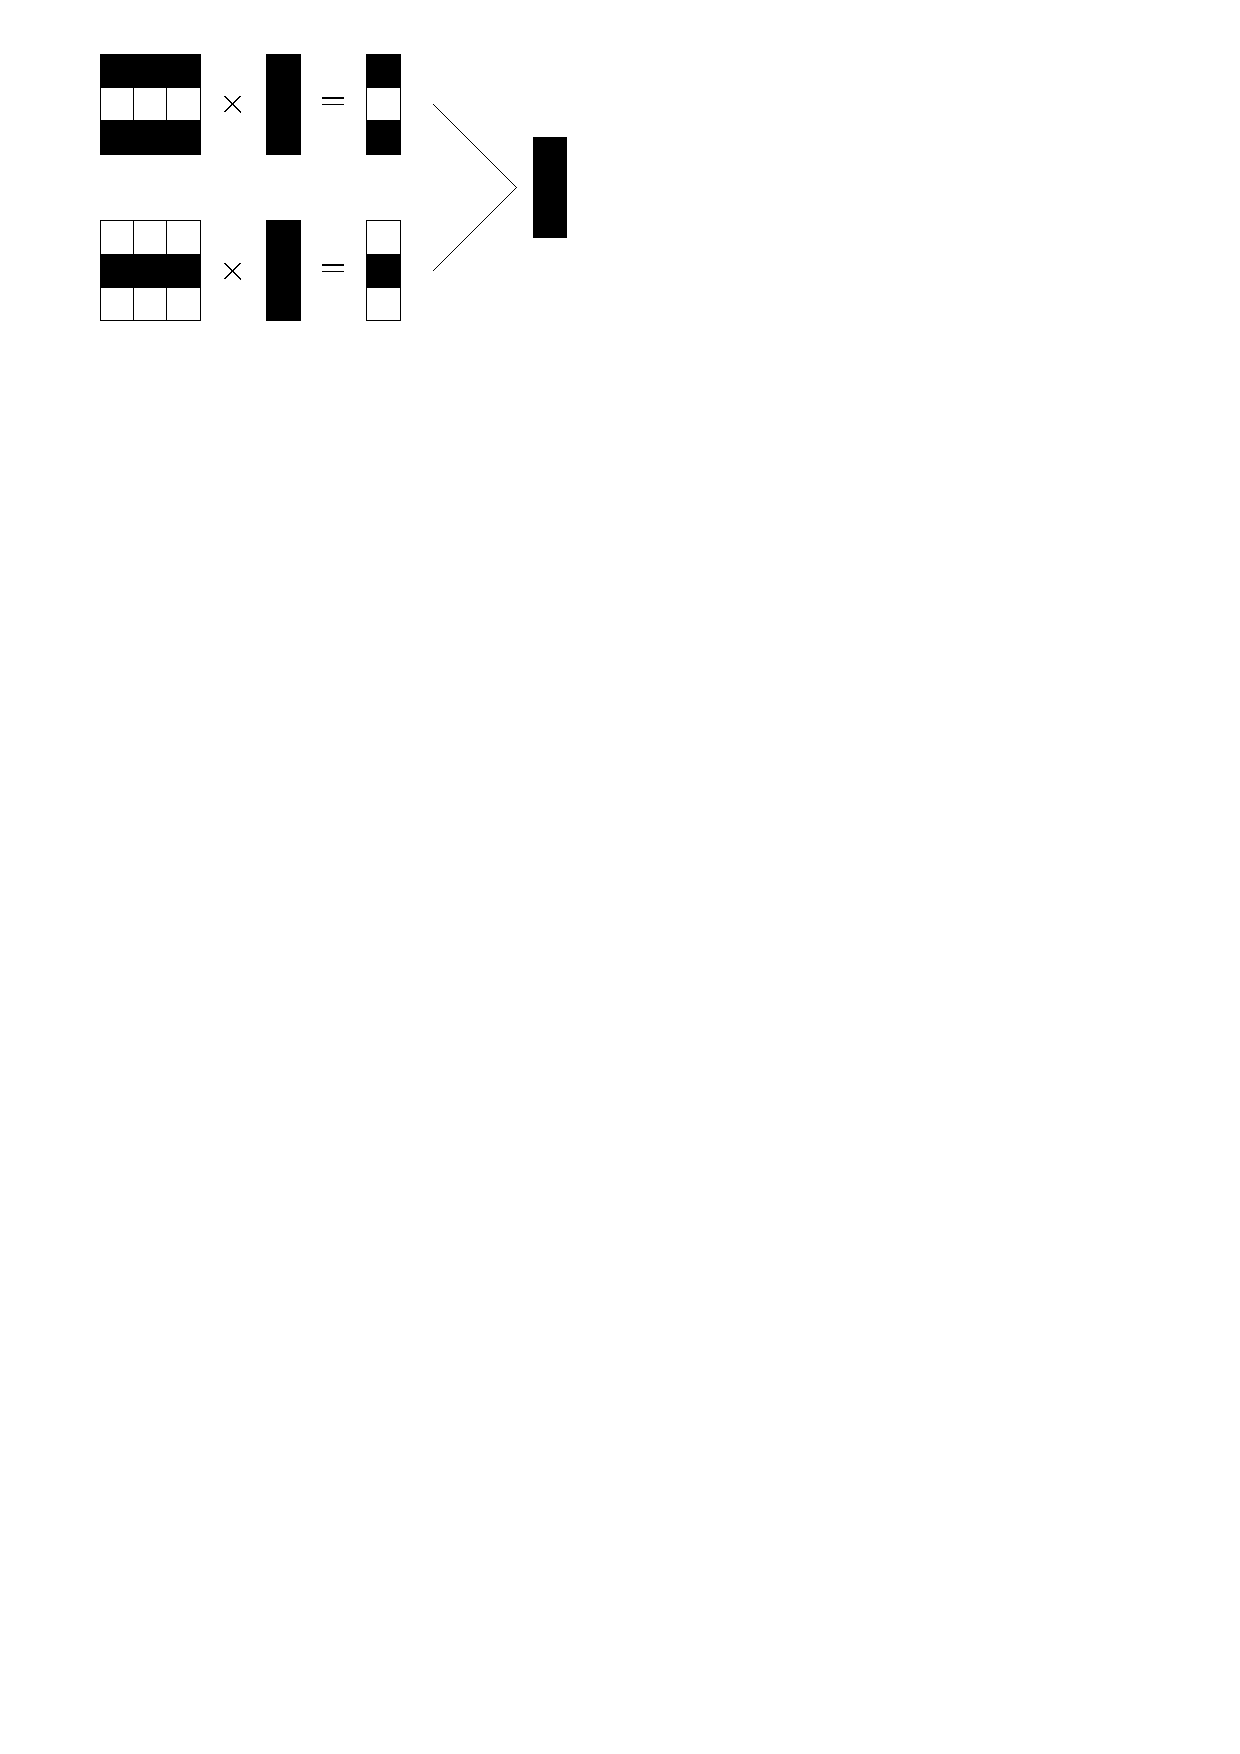
\includegraphics[width=0.5\linewidth]{figs/mmult.pdf}
\end{center}

Je nutné slévat částečné výsledky jednotlivých vláken. Jak na to?
  

\end{frame}

\begin{frame}[fragile]
  \frametitle{Vlastní redukce}
  
  Standardní redukce jsou definované na jednoduchých proměnných.
  
  \begin{center}
  \Large Co když chceme agregovat výsledky ve složitější datové struktuře?
  \end{center}
  
  \pause
  
  \hfill Deklarujeme si vlastní redukci!
  
  \pause
  
  \begin{minted}{c}
  #pragma omp declare reduction(name:type:expression) \ 
  	initializer(expression)
 \end{minted}
 \pause
 \begin{itemize}
 \item name = název vlastní redukce
 \item type = typ, nad kterým je redukce definována (např. std::vector<int>)
 \item expression = funkce, která se má vykonávat nad dvěma částečnými výsledky 
 \end{itemize}
 \pause
 $\rightarrow$ částečné výsledky jsou uložené v proměnných \texttt{omp\_in} a \texttt{omp\_out}
 
  $\rightarrow$ výsledek redukce uložíme zpět do proměnné \texttt{omp\_out}
 \pause
  \begin{itemize}
 \item initializer = jaká má být počáteční hodnota lokální kopie redukované proměnné v každém vlákně
       (lokální proměnná = \texttt{omp\_priv})
 \end{itemize} 

\end{frame}

{\setbeamertemplate{frame footer}{\see{{\tt multiply.cpp} \sep {\tt make mult}}}
\begin{frame}[fragile]

  \begin{minted}{c}
  void merge_elements(element_t & dest, element_t & in) {
  	dest = gcd(dest,in); }
  ...
  #pragma omp declare reduction(merge : \
                                element_t : \
                                merge_elements) \
  	                  initializer(omp_priv = 0)
  element_t result;
  #pragma omp parallel for reduction(merge : result)
  for(int i = 0; i < size, i++{
  // do something with result
  }
 \end{minted}
 
  \vspace{1em}\pause\hrule\vspace{1em}

  \begin{block}{Doimplementujte násobení matice s vektorem}
    Doimplementujte tělo metody \texttt{multiply\_parallel}. Vlastní redukci jsme vám již deklarovali. Redukce využívá funkci \texttt{merge}. Doimplementujte i tělo redukce (funkce \texttt{merge}). Všechny vektory se kterými pracujete jsou řídké!
  \end{block}

\end{frame}
}

\section{Semestrální úloha}

\begin{frame}
  \frametitle{Stavové prostory}
  
   \begin{minipage}{0.5\linewidth}
   Diskrétní dynamické systémy mají různé \textit{konfigurace}
   
    \vspace{1em}
 
    Mezi konfiguracemi lze přecházet\\ pomocí akcí
    
    \vspace{4em}\hrule\vspace{2em}
 
    \hfill{\bf Jak takové systémy vypadají?}
  \end{minipage}
  \hfill
  \begin{minipage}{0.4\linewidth}
    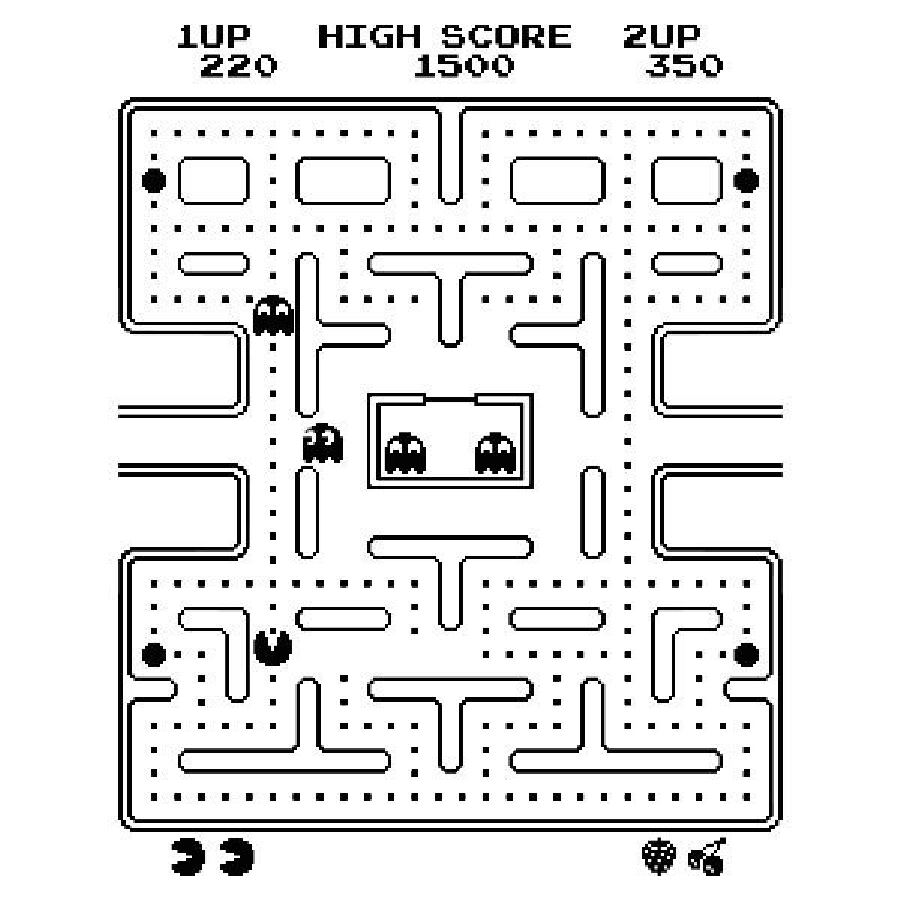
\includegraphics[width=1.1\linewidth]{figs/pacman2.pdf}
  \end{minipage}
 
  

\end{frame}

\begin{frame}
  \frametitle{Hanojské věže}
  
  Přesouváme věže z disků z {\bf počátečních} kolíků na {\bf koncové}.
  
  \begin{itemize}
  \item Jen jeden disk v jednom kroku
  \item Větší disk nemůže být na menším
  \end{itemize}
  
  \vspace{1em}

\begin{center}
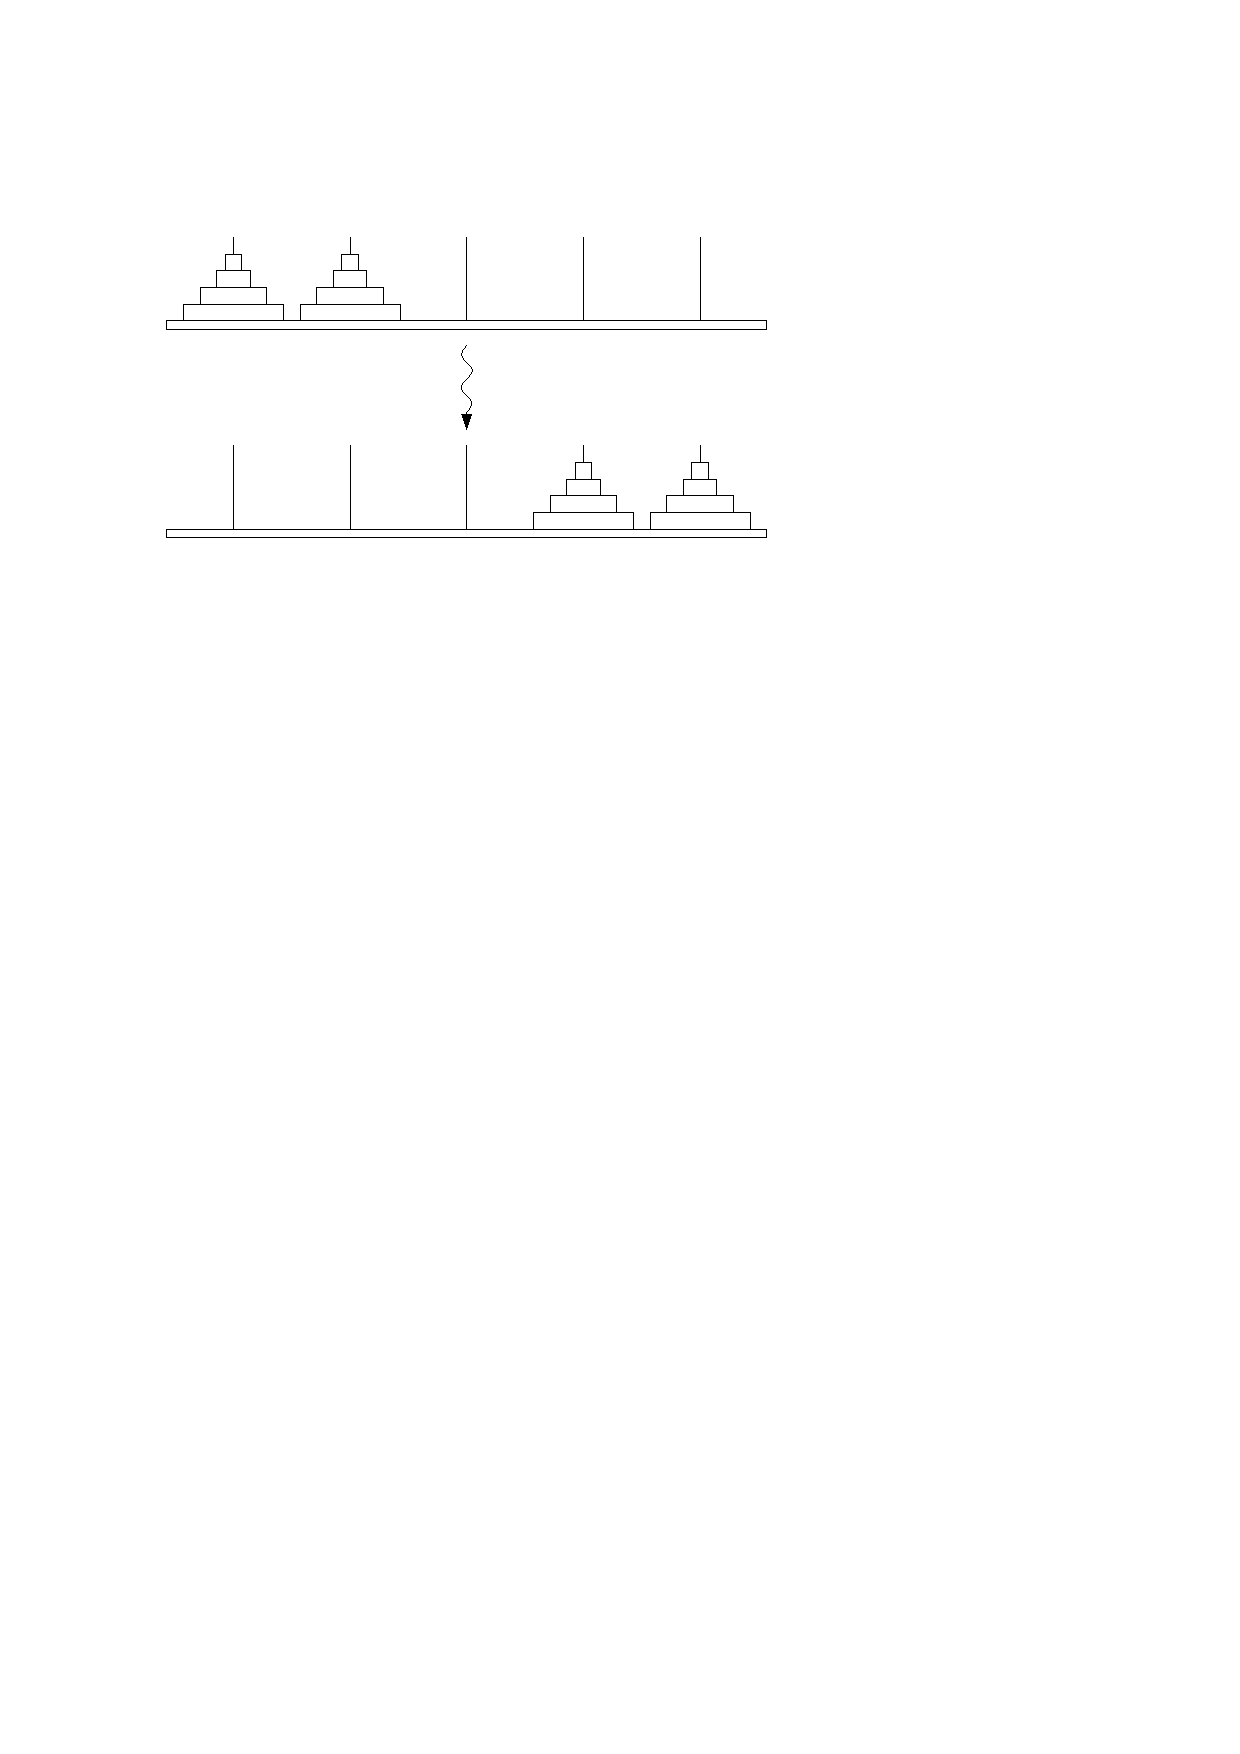
\includegraphics[width=0.5\linewidth]{figs/hanoi.pdf}
\end{center}

\vspace{1em}\hrule\vspace{1em}

\faWarning\hspace{3pt} Doména je korektní, pokud $DISCS*TOWERS*ceil(\log_2(RODS)) \leq 64$.

\end{frame}

\begin{frame}
  \frametitle{Loydův hlavolam (``sliding puzzle'')}
  
  Přesouváme X po poli abychom se dostali z počáteční konfigurace na setříděnou.
  
  \begin{itemize}
  \item Jen jedno prohození v jednom kroku.
  \item Prohodíme X s poličkem o jedno nahoře, dole, vlevo nebo vpravo.
  \end{itemize}
  
  \vspace{1em}

\begin{center}
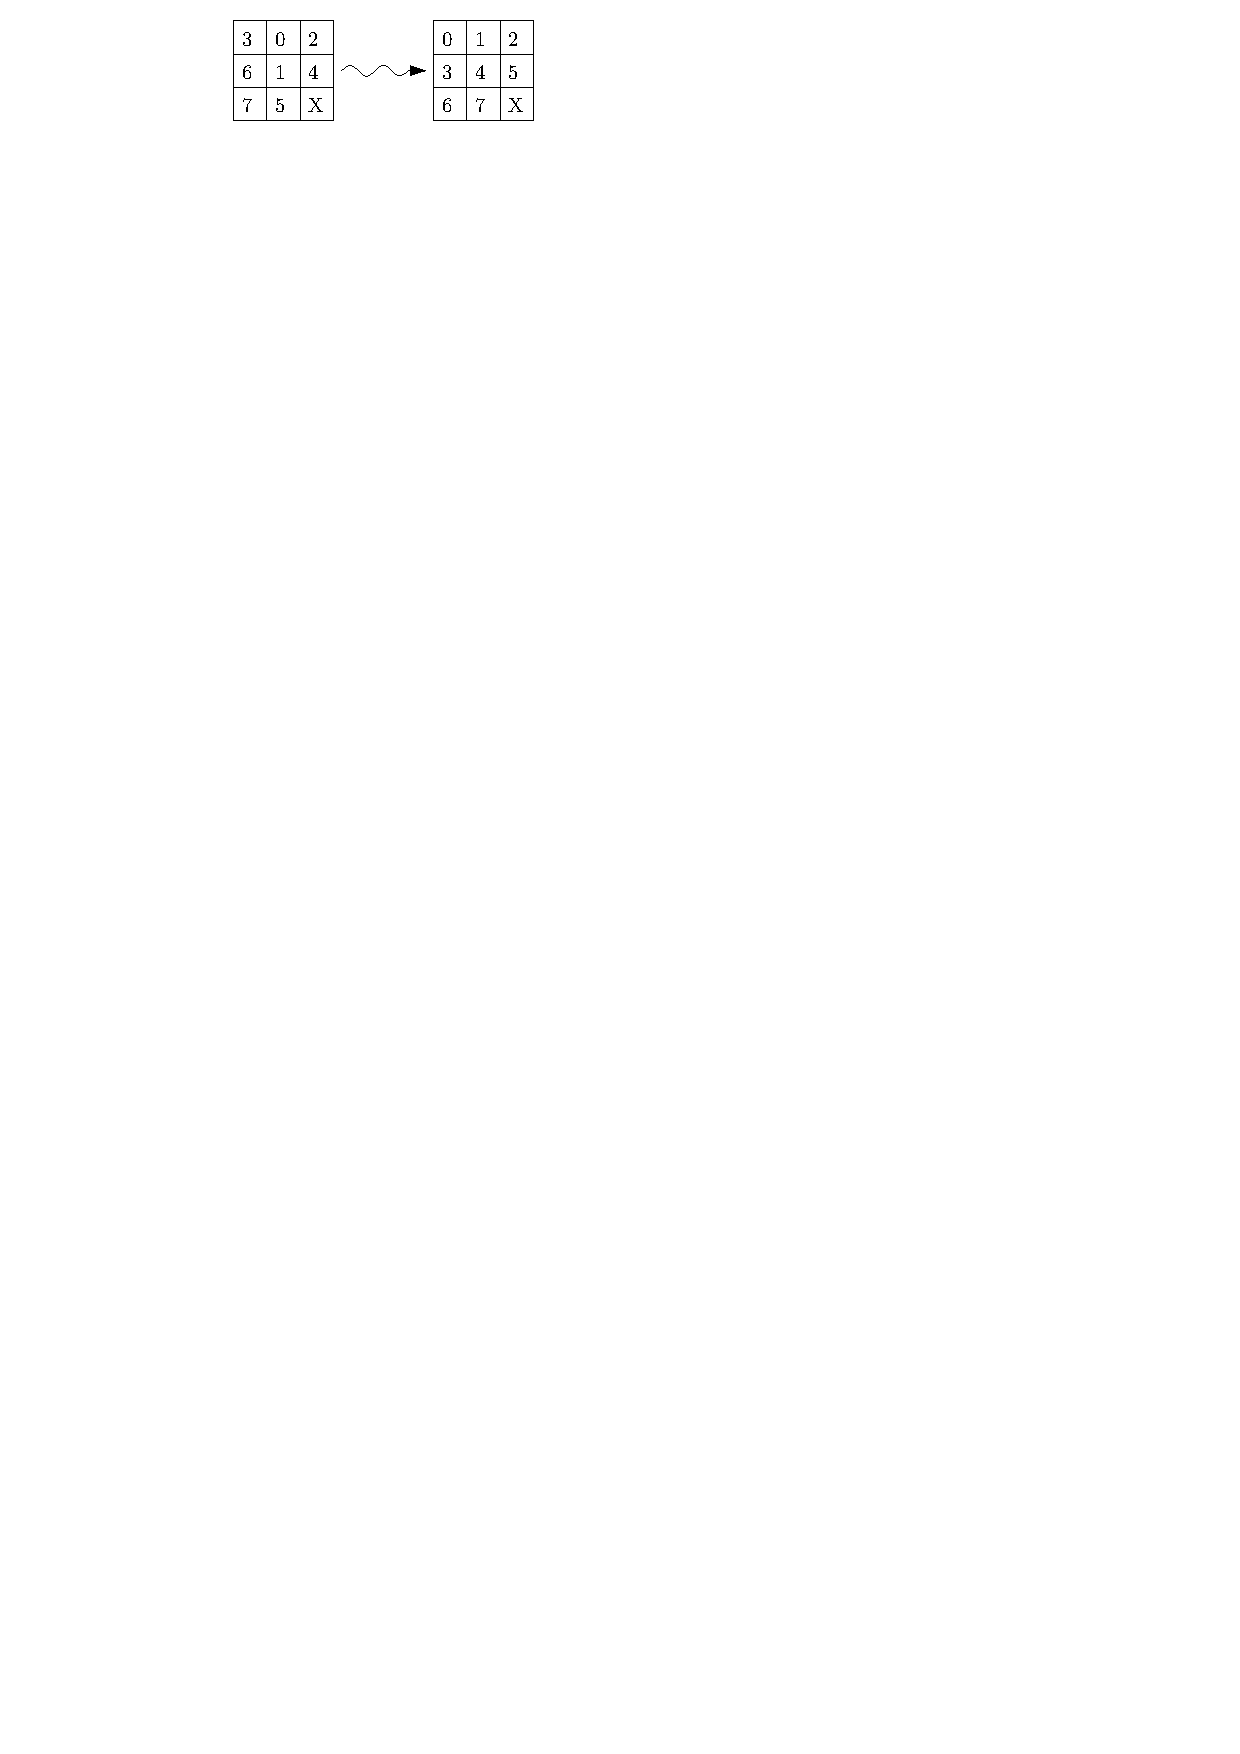
\includegraphics[width=0.5\linewidth]{figs/sp.pdf}
\end{center}

\vspace{1em}\hrule\vspace{1em}

\faWarning\hspace{3pt} Doména je korektní pro rozměry pole $3\times 3$ a $4\times 4$.

\end{frame}

\begin{frame}
  \frametitle{Splňování booleovských formulí (``SAT'')}
  
  Pro danou formuli v {\bf konjunktivním normálním tvaru} hledáme ohodnovení, ve kterém bude {\bf splněná}.
  
  \begin{equation*}
  (\neg x\vee \neg y)\wedge y
  \end{equation*}
  
  \begin{itemize}
  \item Přiřazení ohodnocení jen jedné proměnné v jednom kroku.
  \item Přiřadíme hodnotu jakékoli proměnné s indexem větším než proměnná ohodnocená v minulém kroku.
  \end{itemize}
  
  \vspace{1em}

\begin{center}
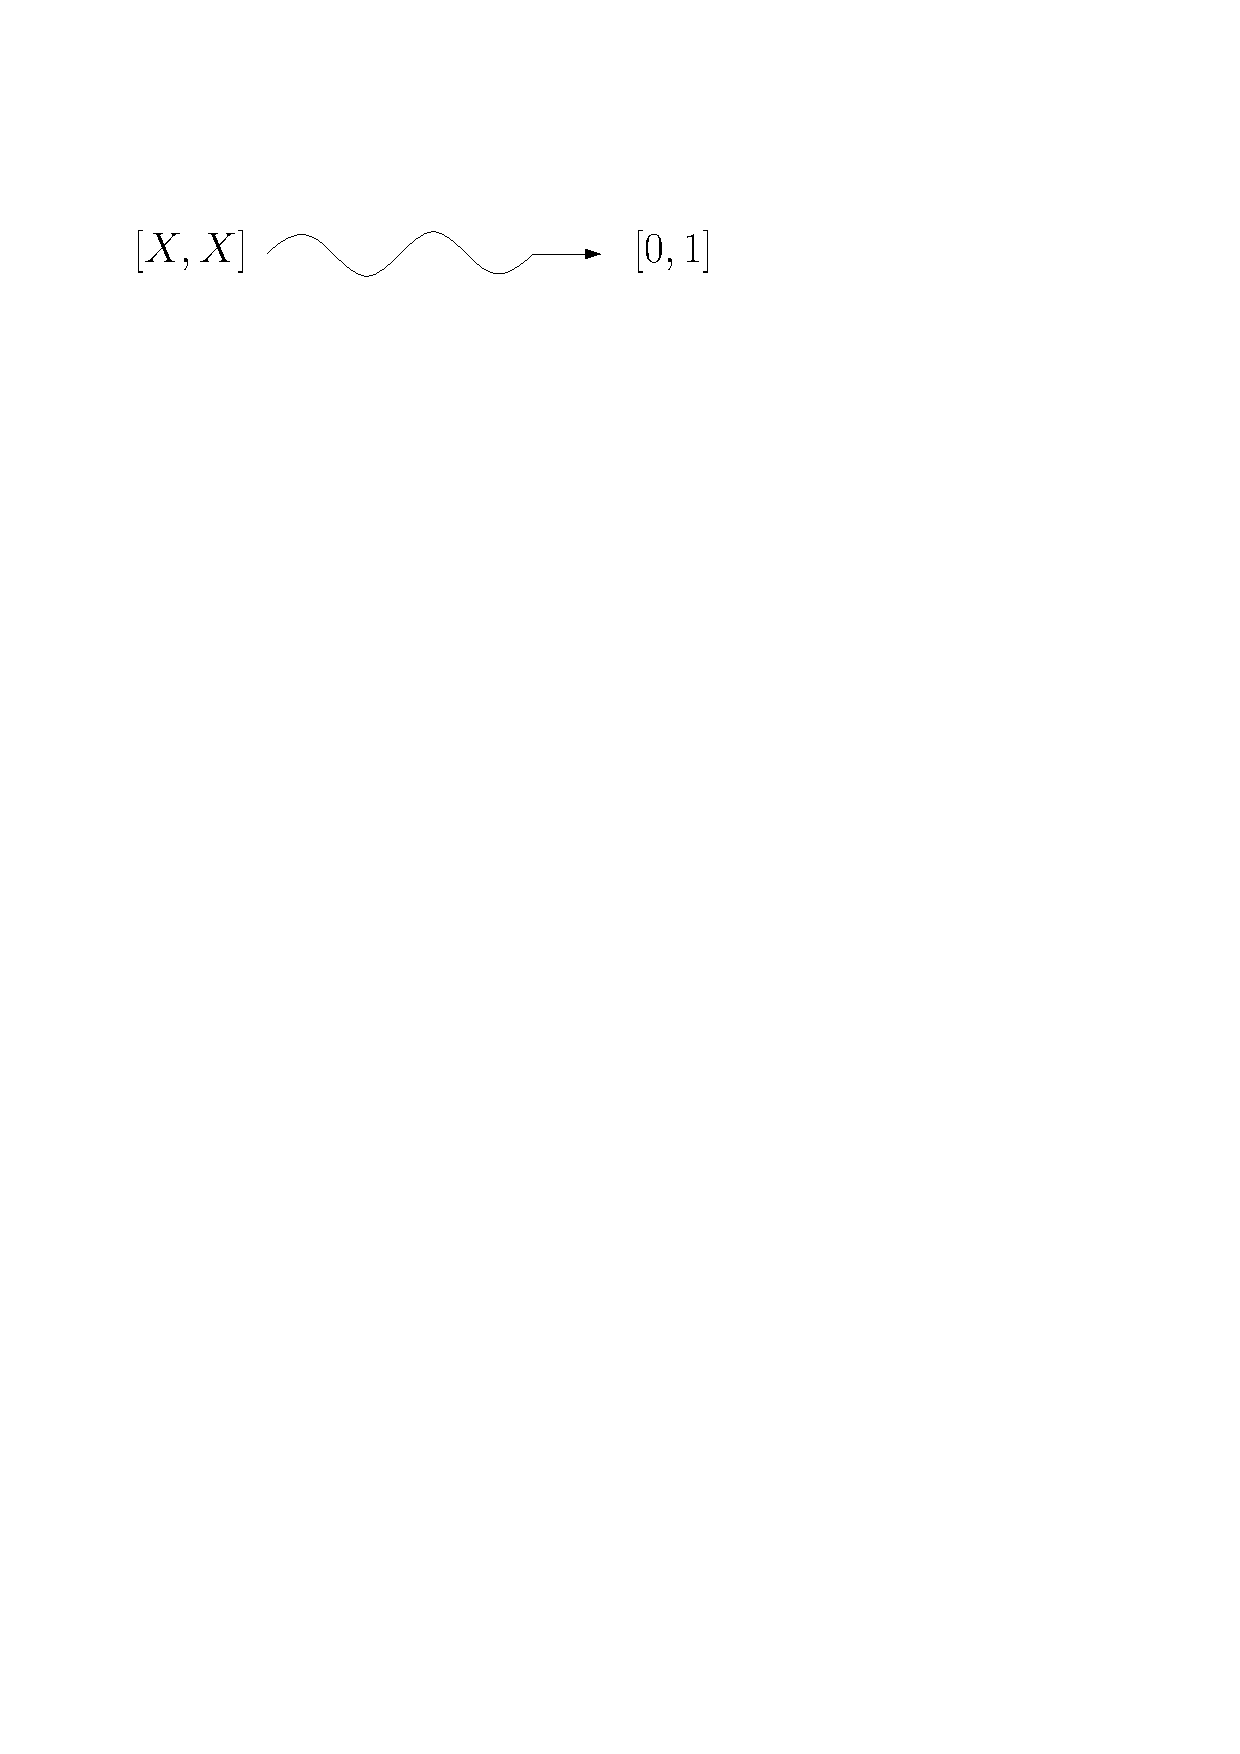
\includegraphics[width=0.5\linewidth]{figs/sat.pdf}
\end{center}

\vspace{1em}\hrule\vspace{1em}

\faWarning\hspace{3pt} Doména je korektní, pokud $NUM\_VARS \leq 40$.
\end{frame}

\begin{frame}
  \frametitle{Bludiště}
  
  Hledáme cestu z počáteční pozice na koncovou.
  
  \begin{itemize}
  \item Pohybujeme se o jedno políčko v každém kroku.
  \item Změníme pozici, pokud nám v cestě nebrání zeď.
  \end{itemize}
  
  \vspace{1em}

\begin{center}
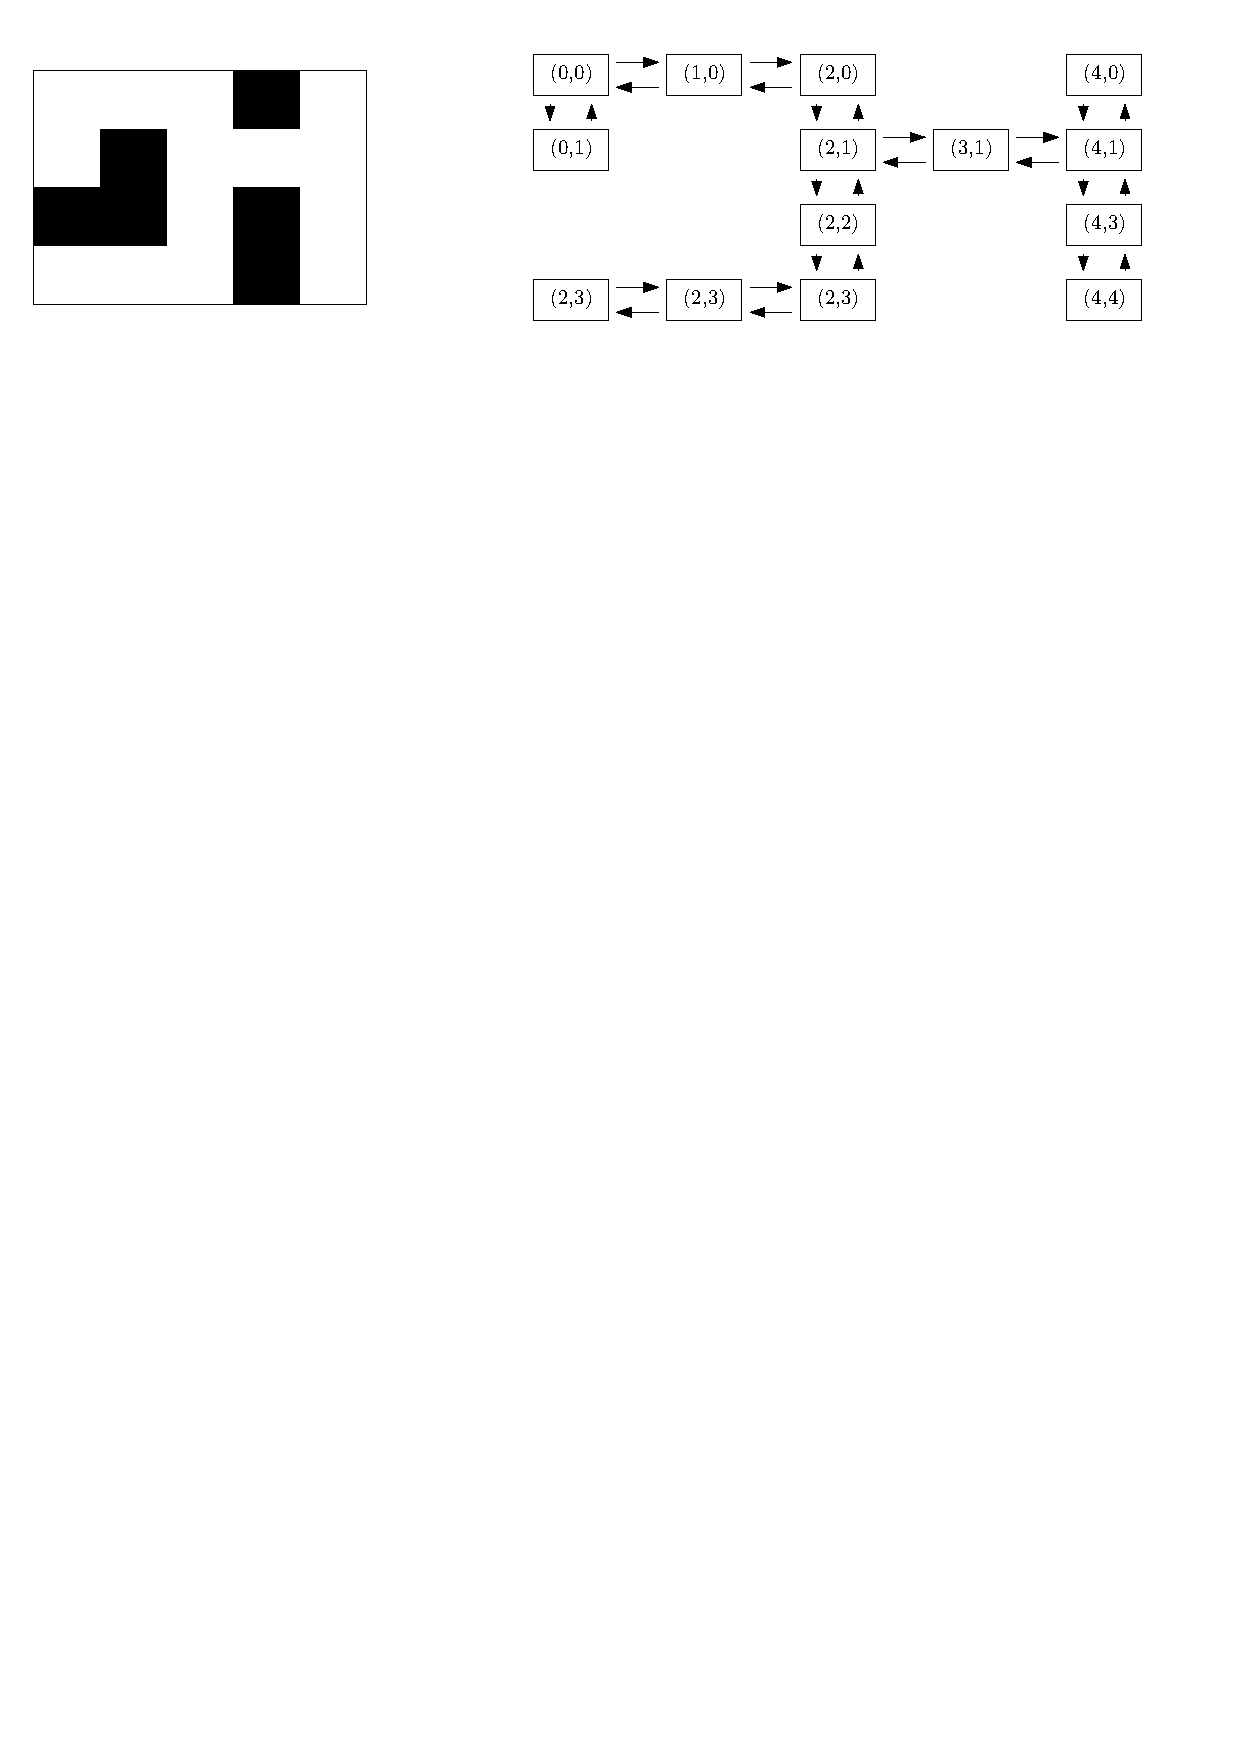
\includegraphics[width=0.9\linewidth]{figs/maze.pdf}
\end{center}

\vspace{1em}\hrule\vspace{1em}

\faWarning\hspace{3pt} Doména je korektní, pokud $\log_2(WIDTH*HEIGHT) \leq 64$.
\end{frame}

\begin{frame}[t]
  \frametitle{Prohledávání do šířky (BFS)}

  \vspace{3em}

  \only<1>{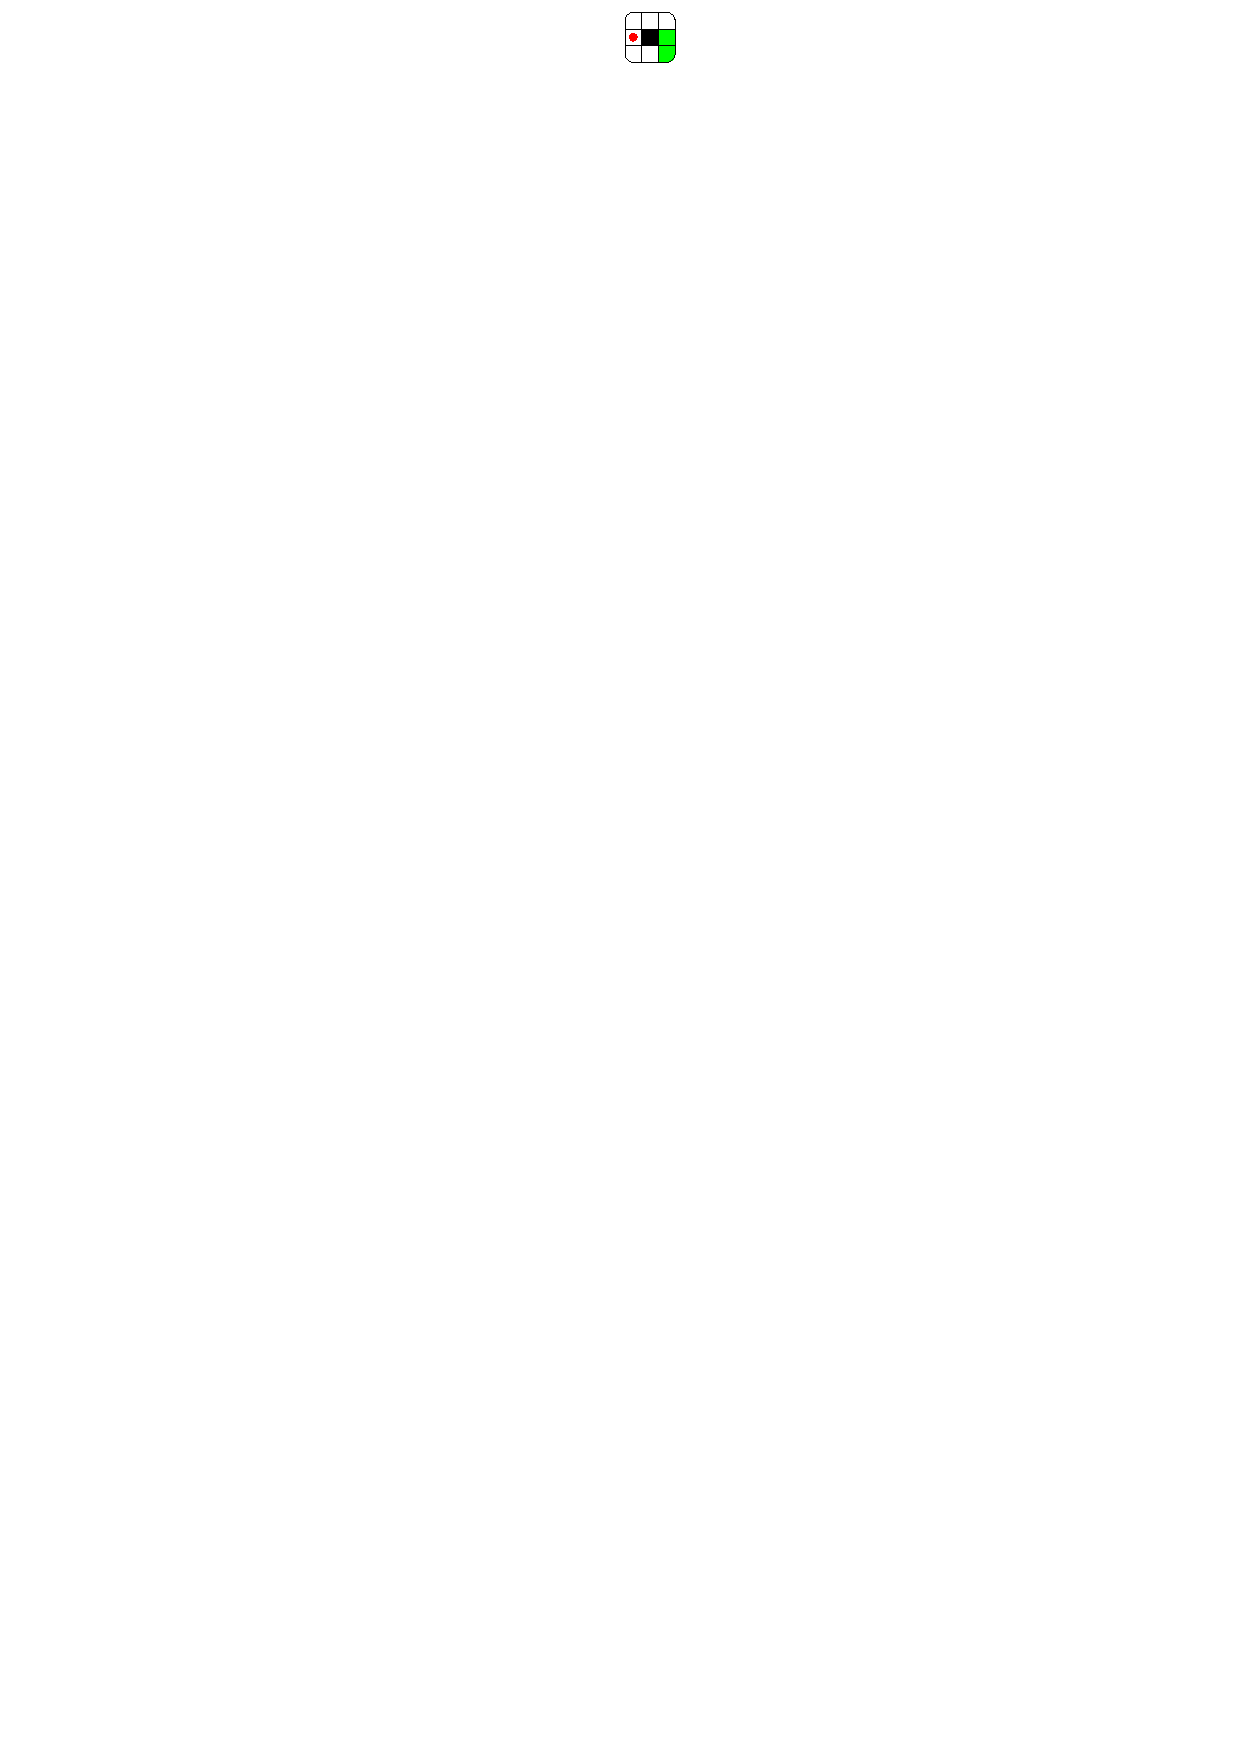
\includegraphics[width=\linewidth]{figs/bfs15.pdf}}%
  \only<2>{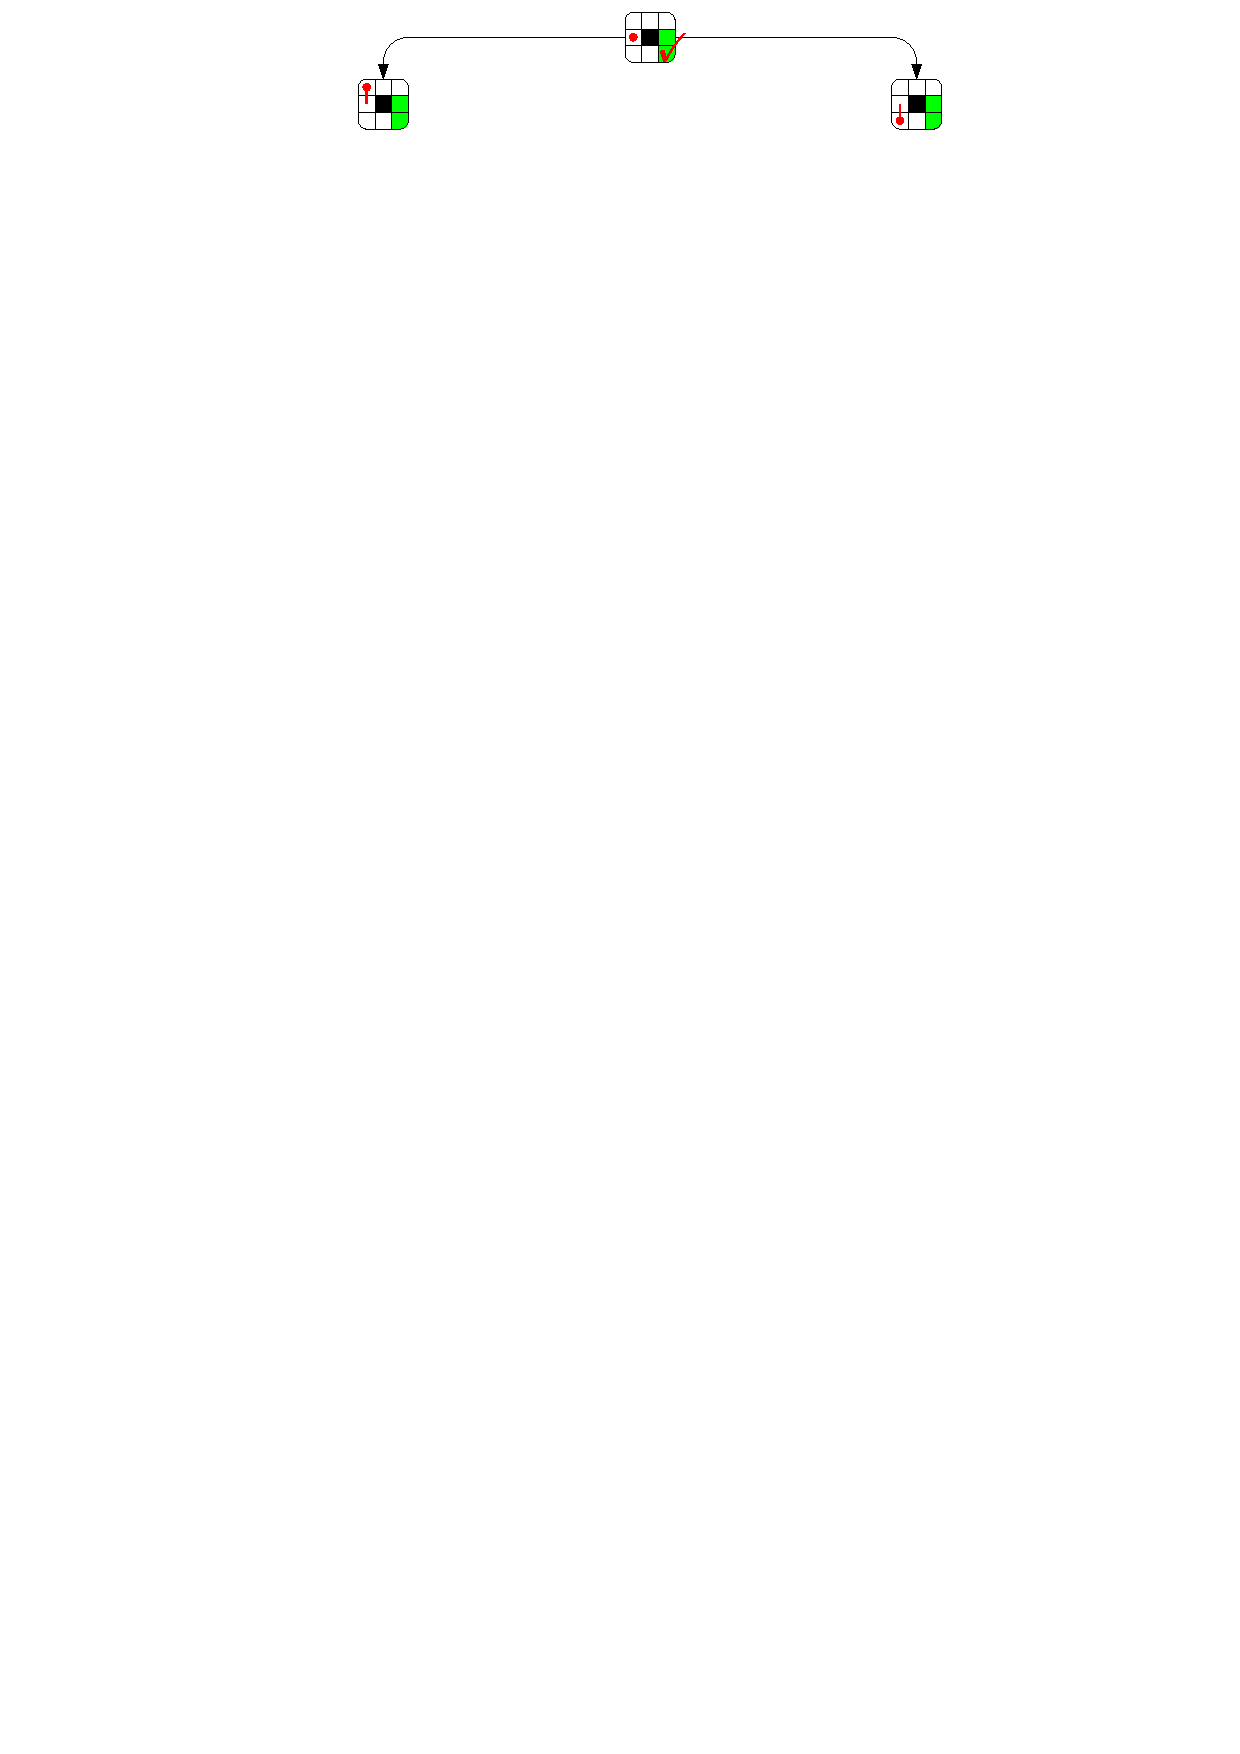
\includegraphics[width=\linewidth]{figs/bfs14.pdf}}%
  \only<3>{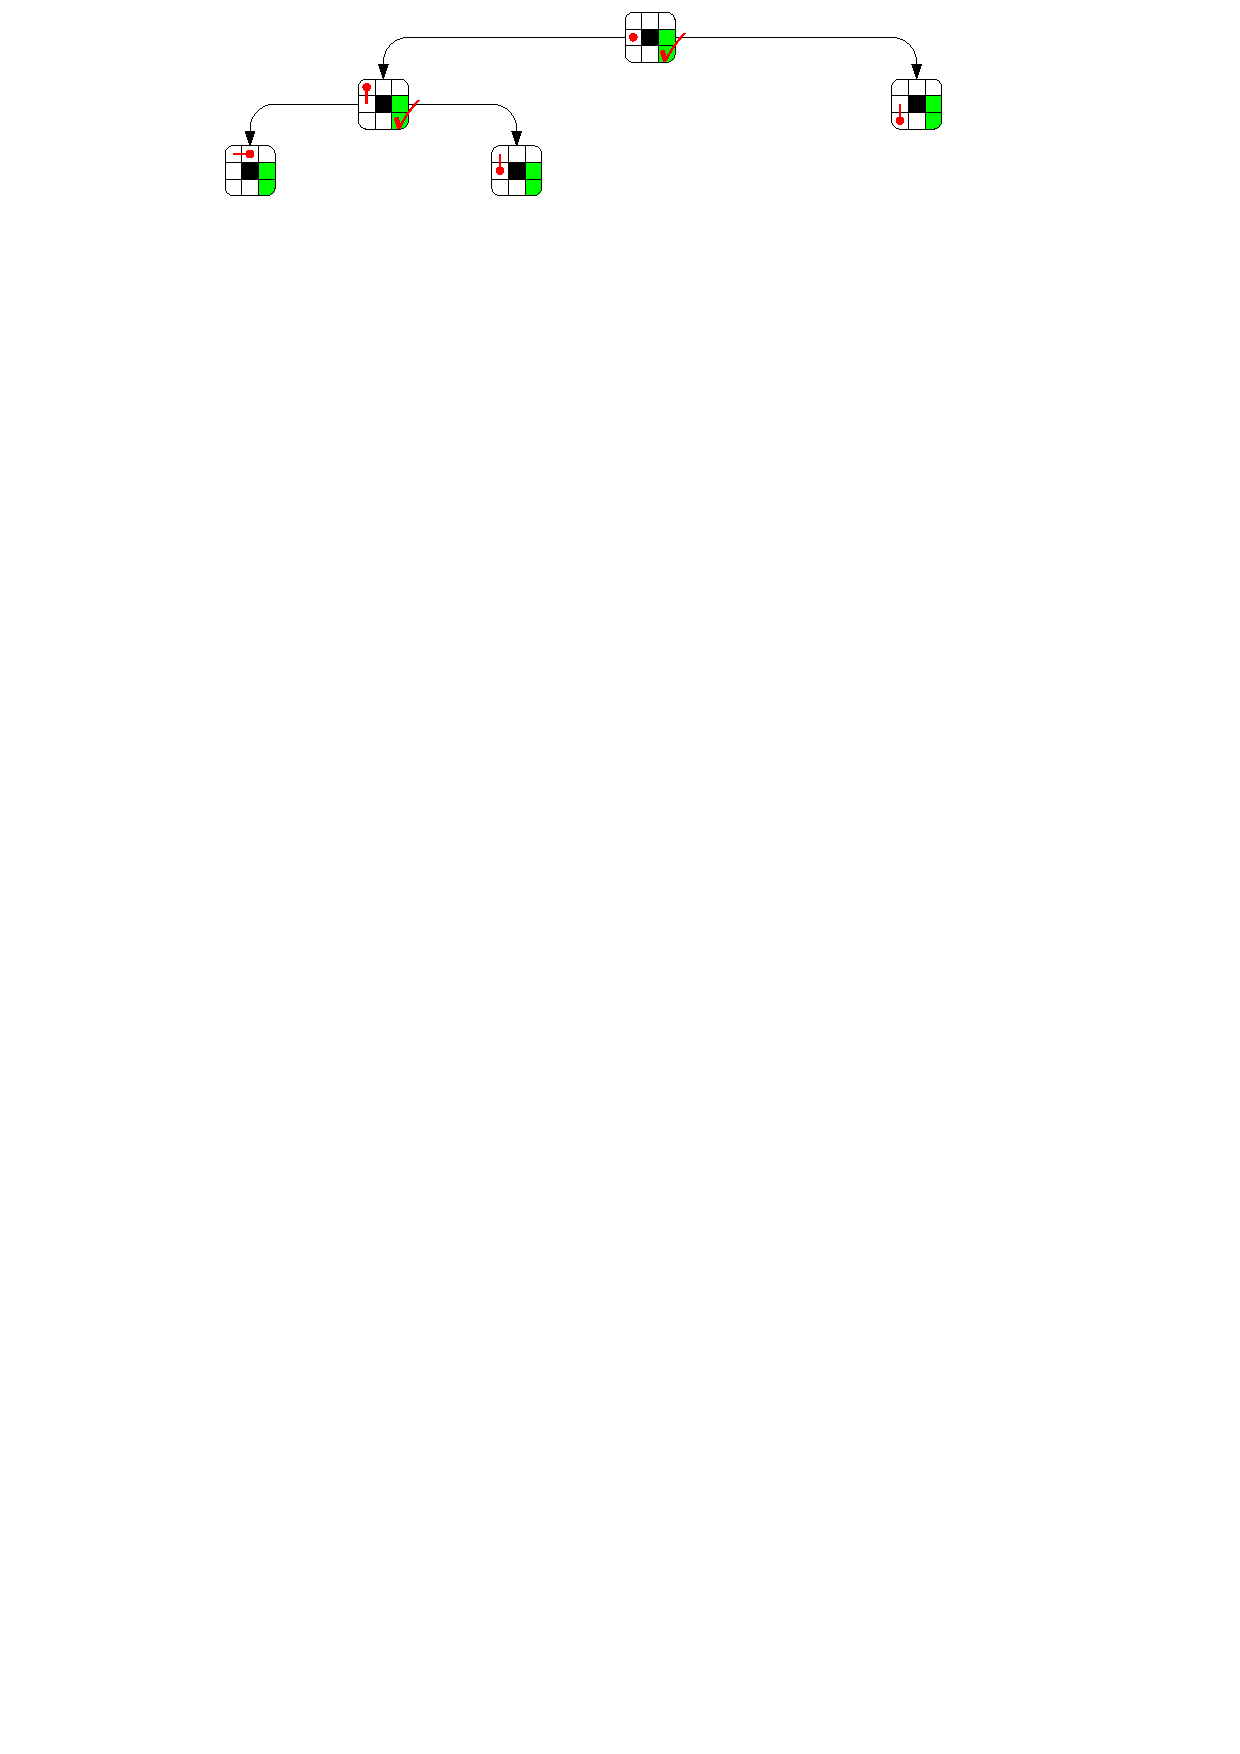
\includegraphics[width=\linewidth]{figs/bfs13.pdf}}%
  \only<4>{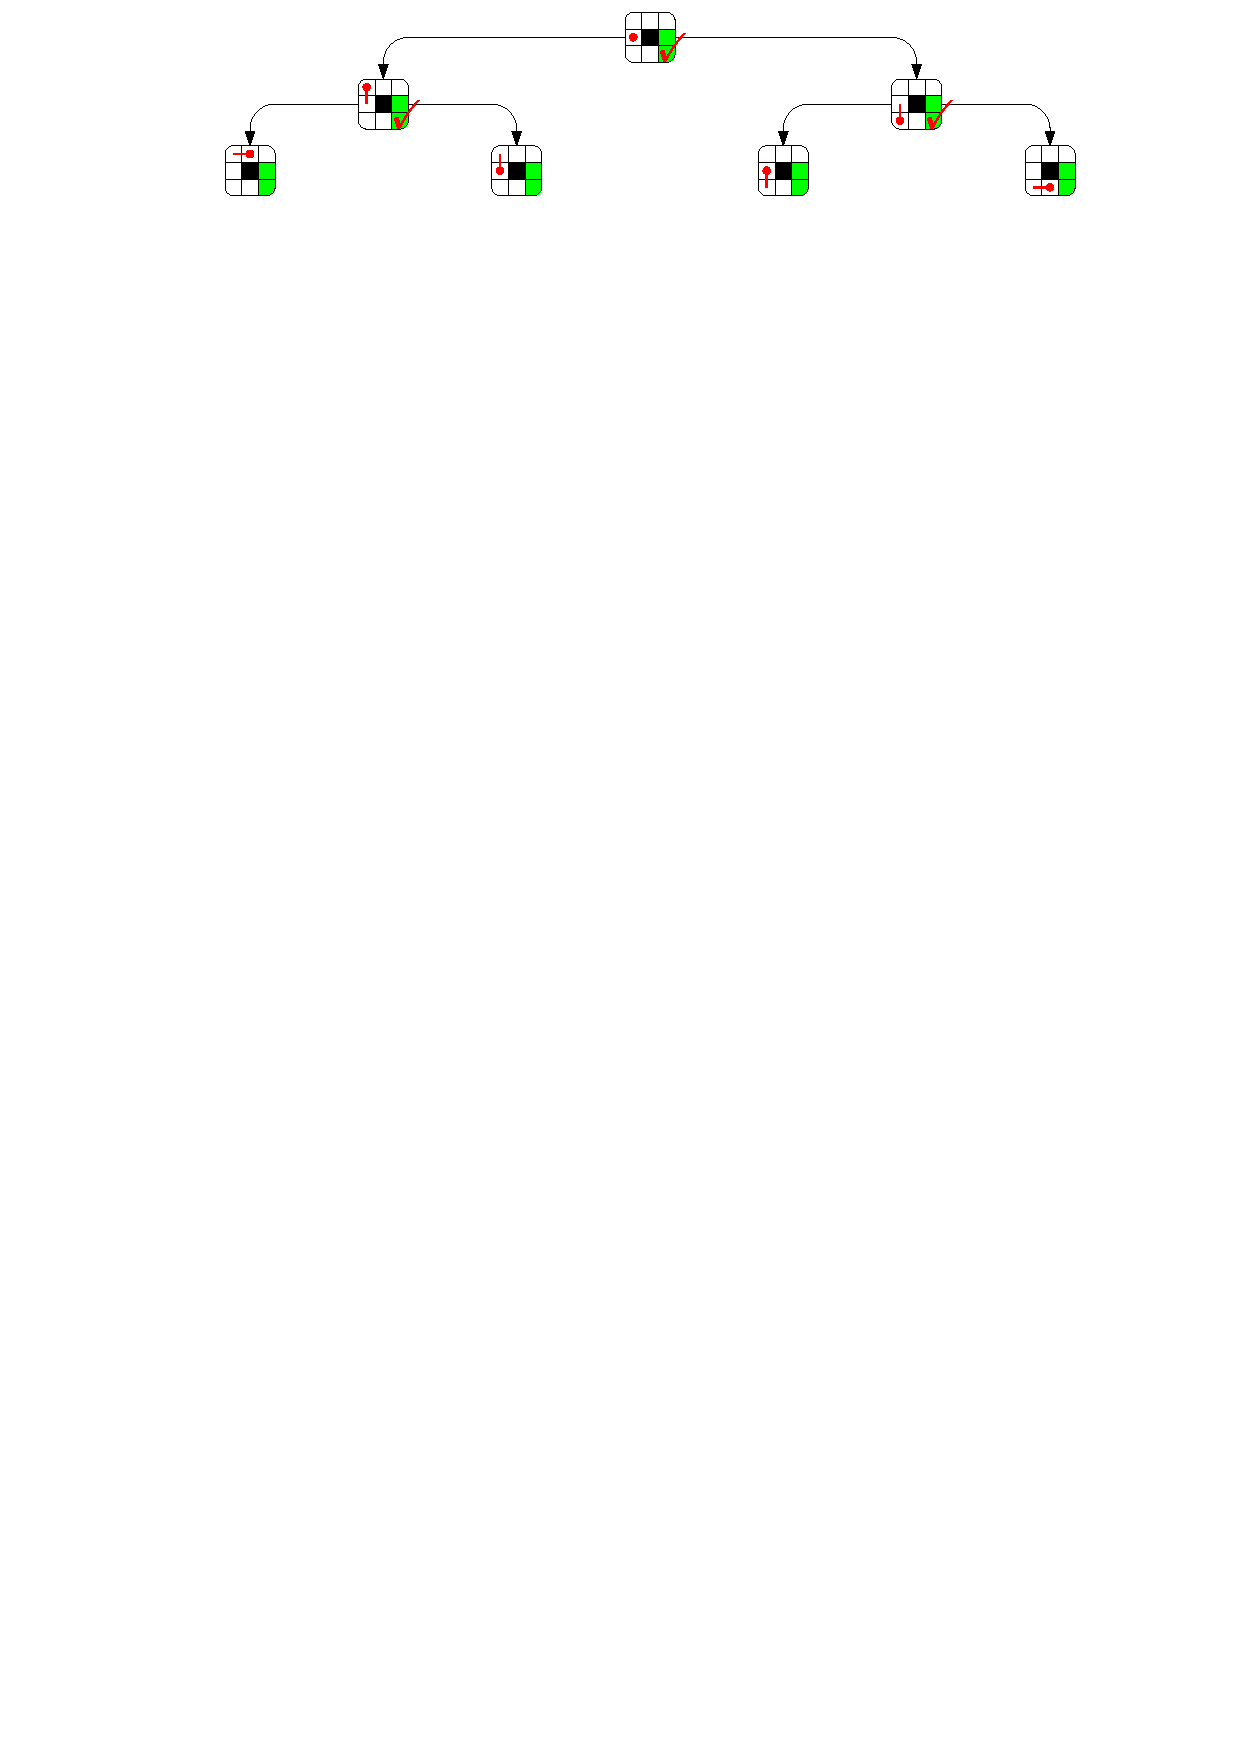
\includegraphics[width=\linewidth]{figs/bfs12.pdf}}%
  \only<5>{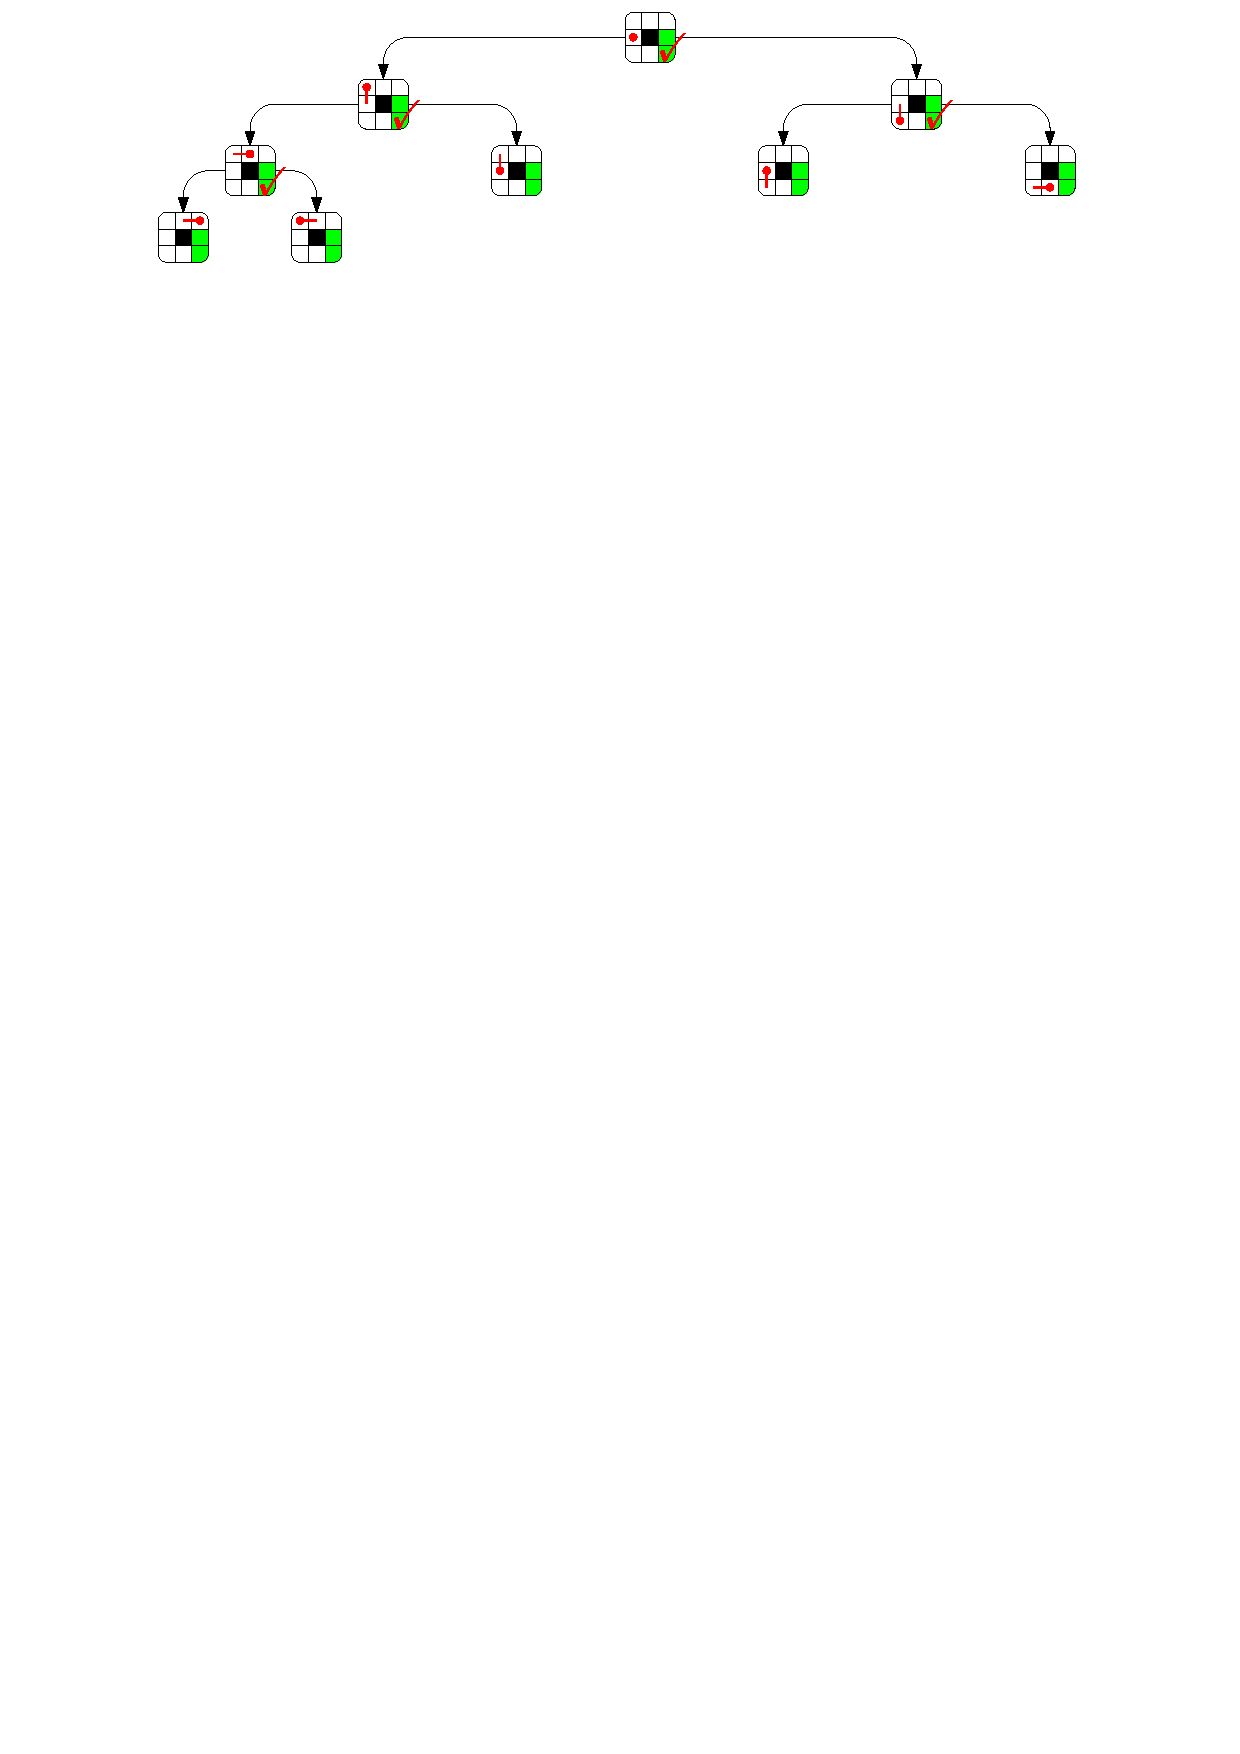
\includegraphics[width=\linewidth]{figs/bfs11.pdf}}%
  \only<6>{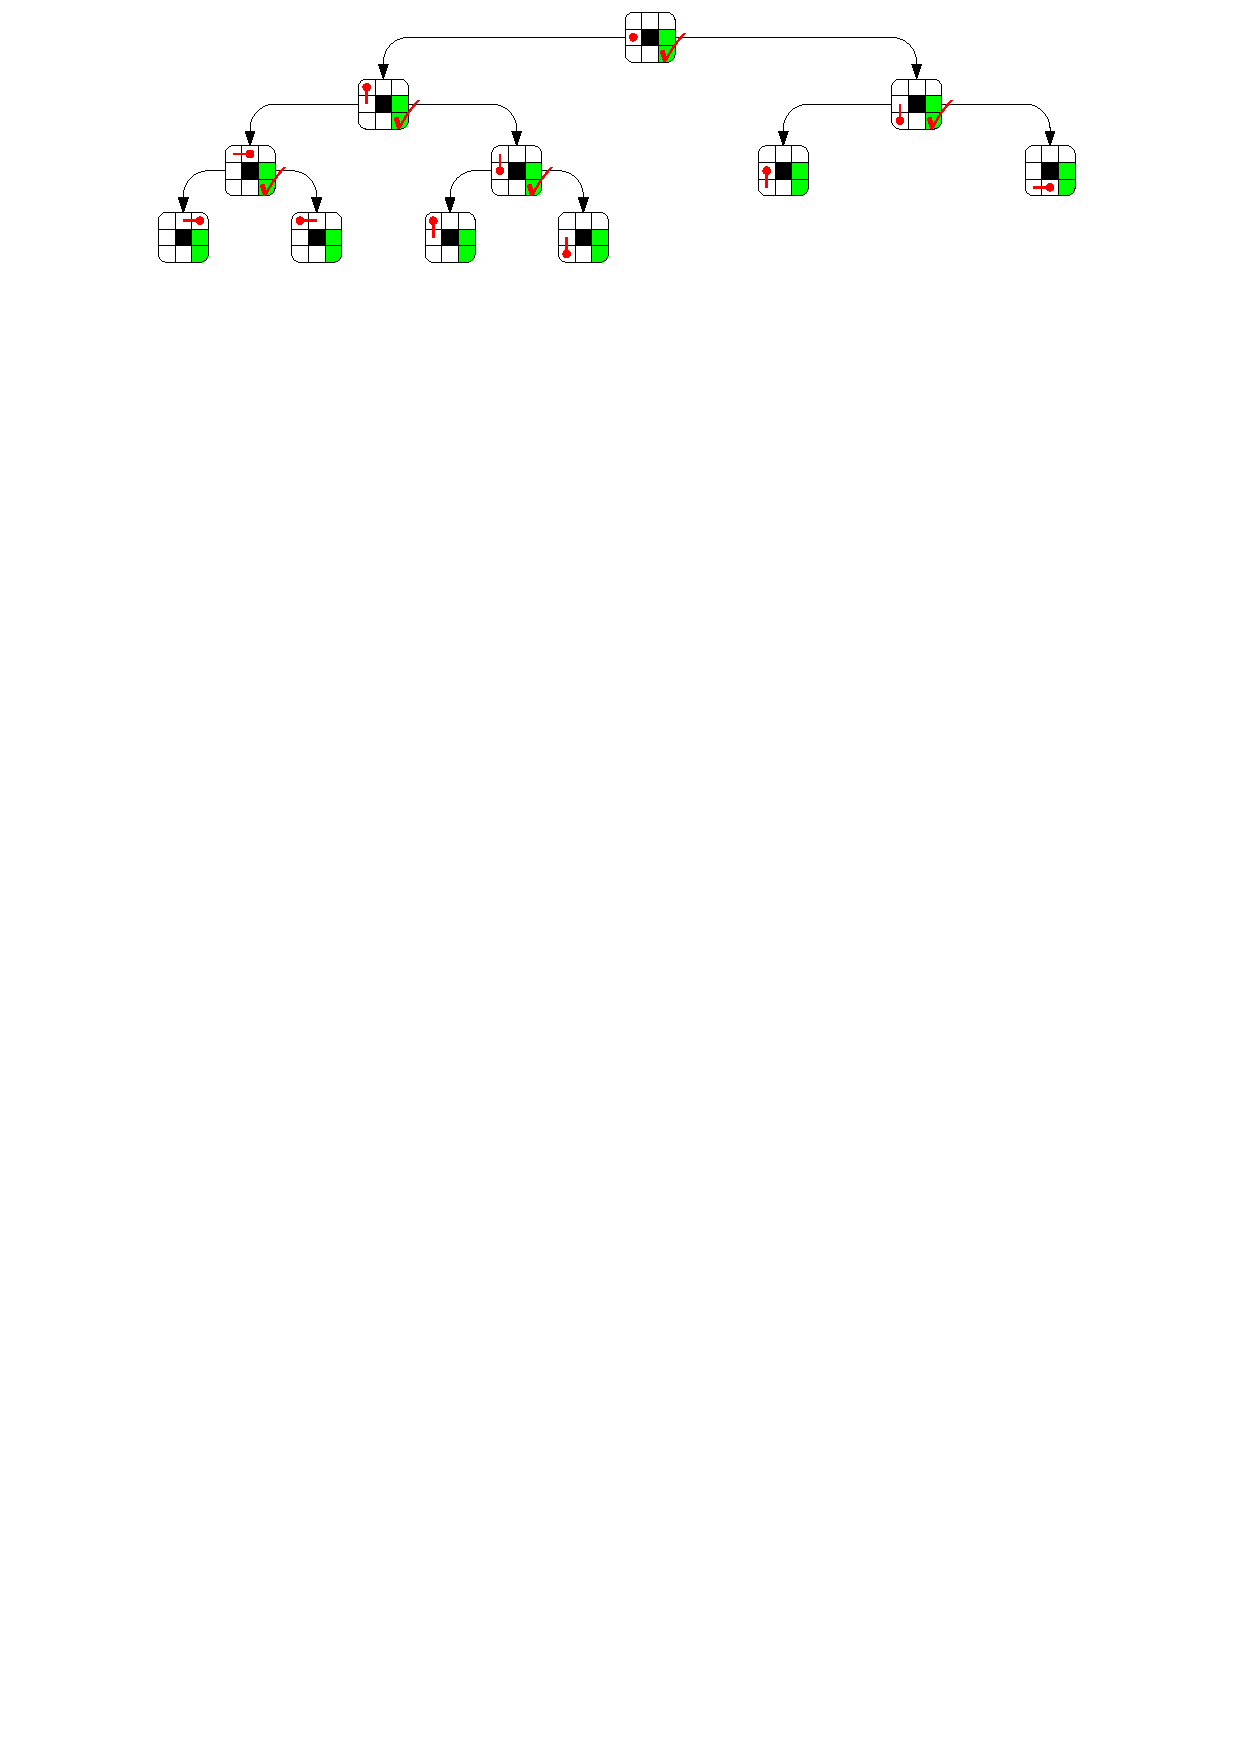
\includegraphics[width=\linewidth]{figs/bfs10.pdf}}%
  \only<7>{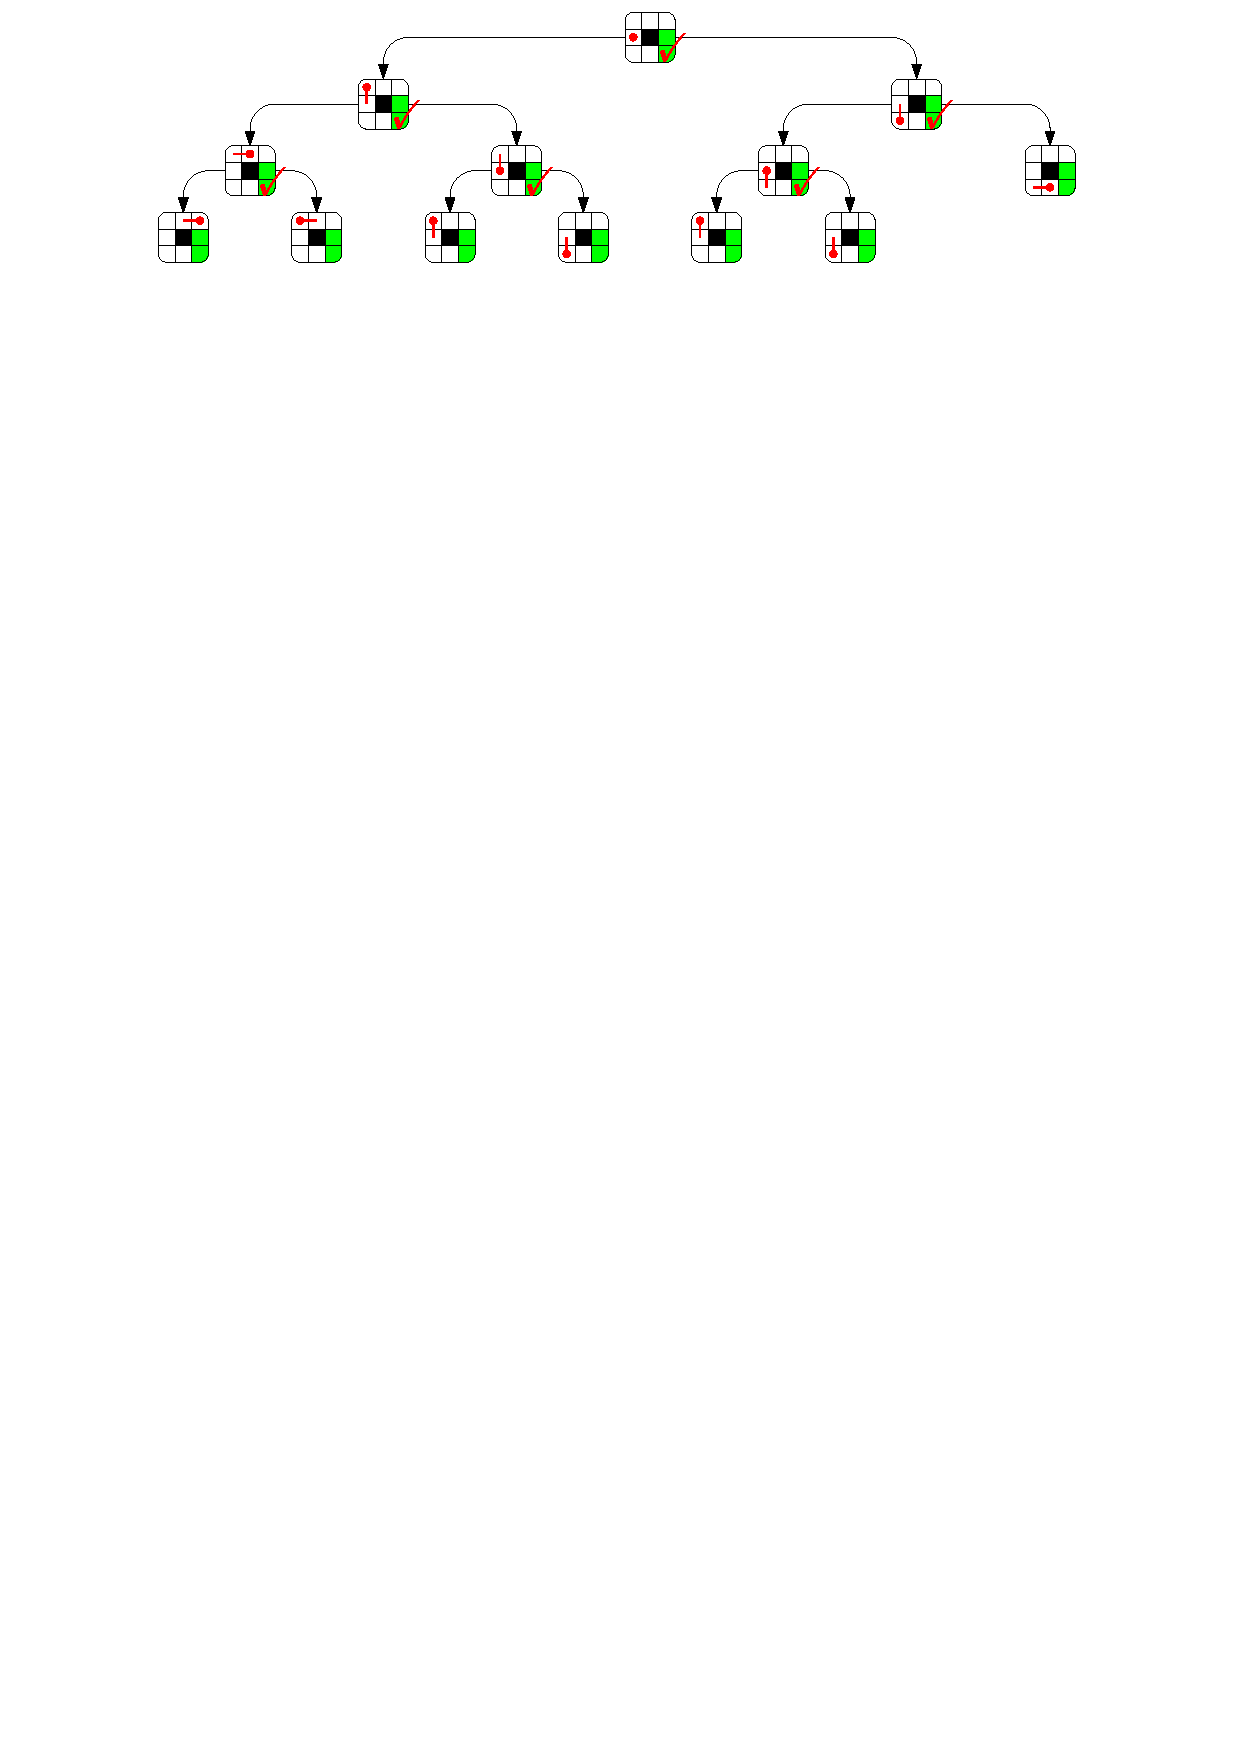
\includegraphics[width=\linewidth]{figs/bfs9.pdf}}%
  \only<8>{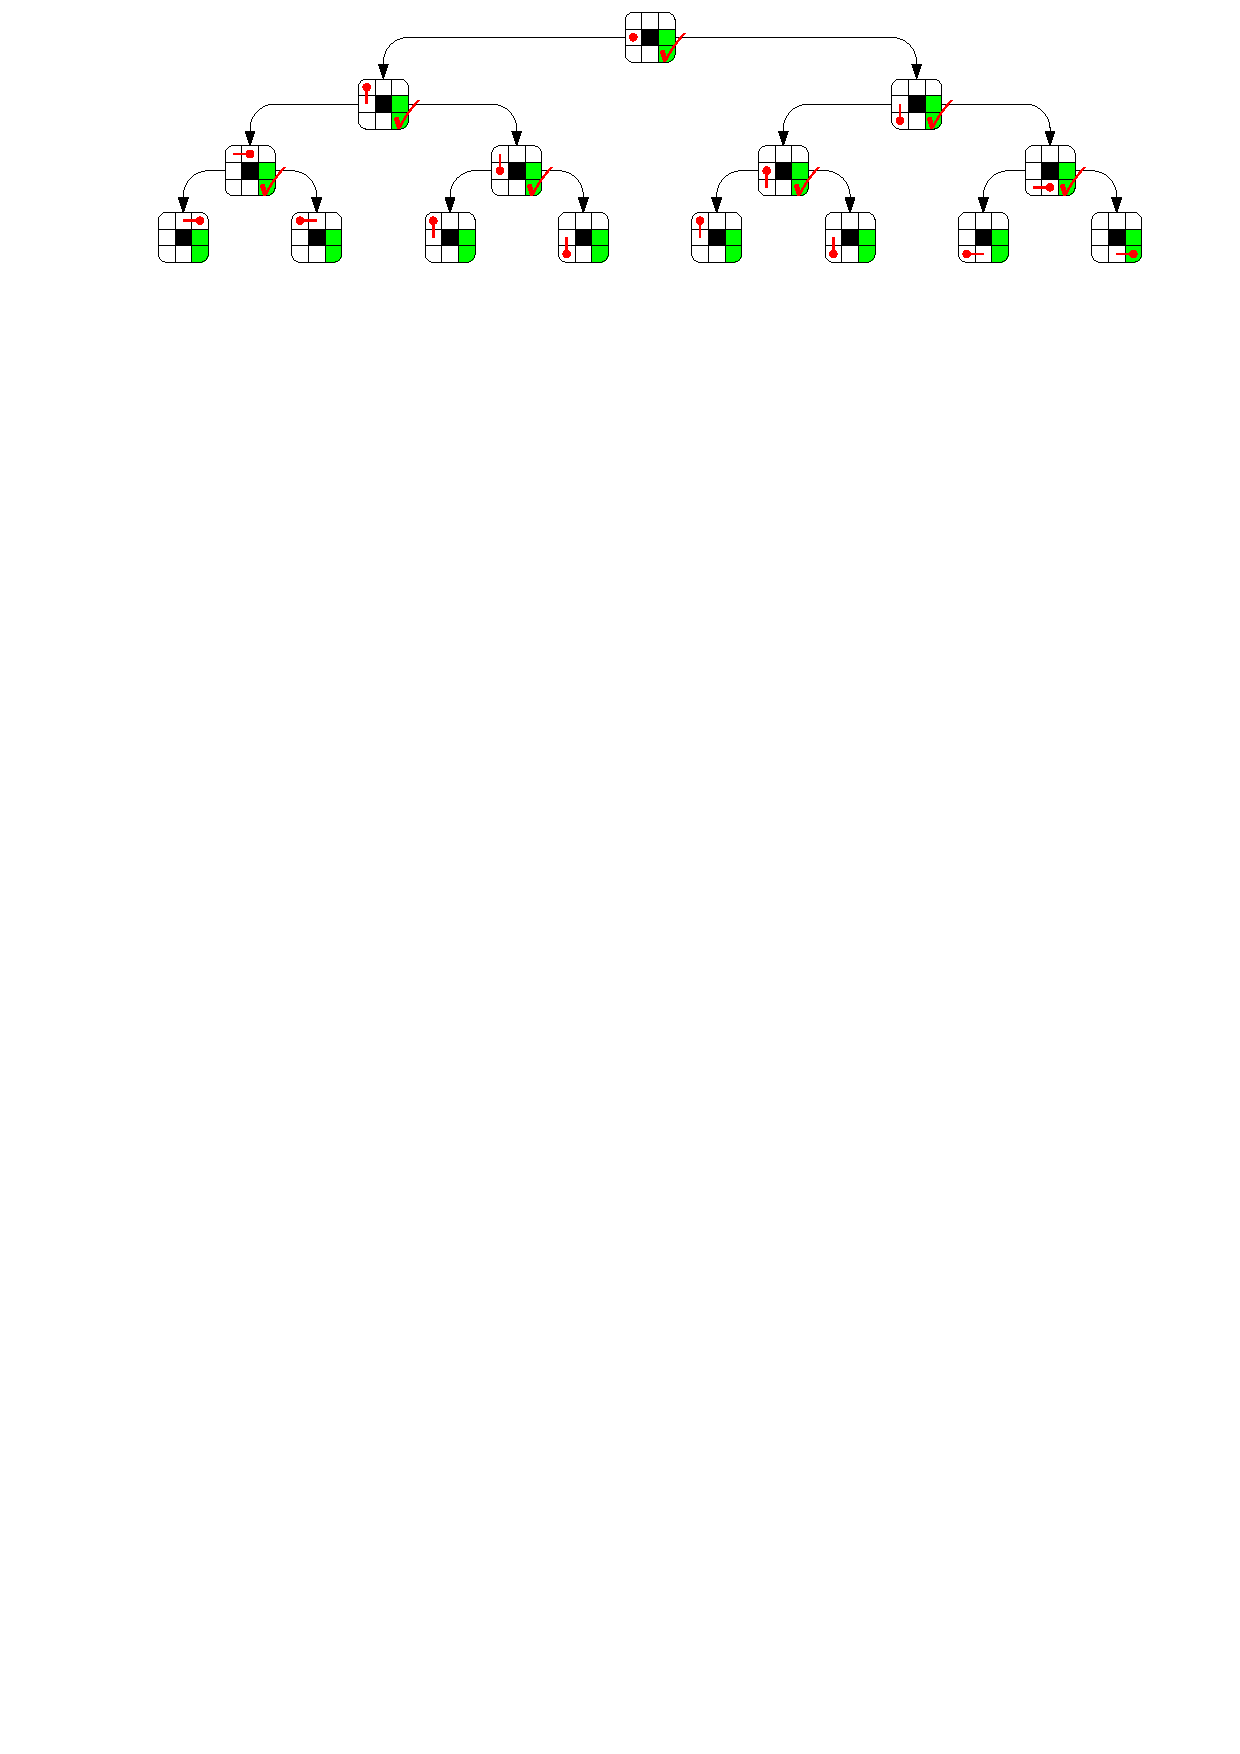
\includegraphics[width=\linewidth]{figs/bfs8.pdf}}%
  \only<9>{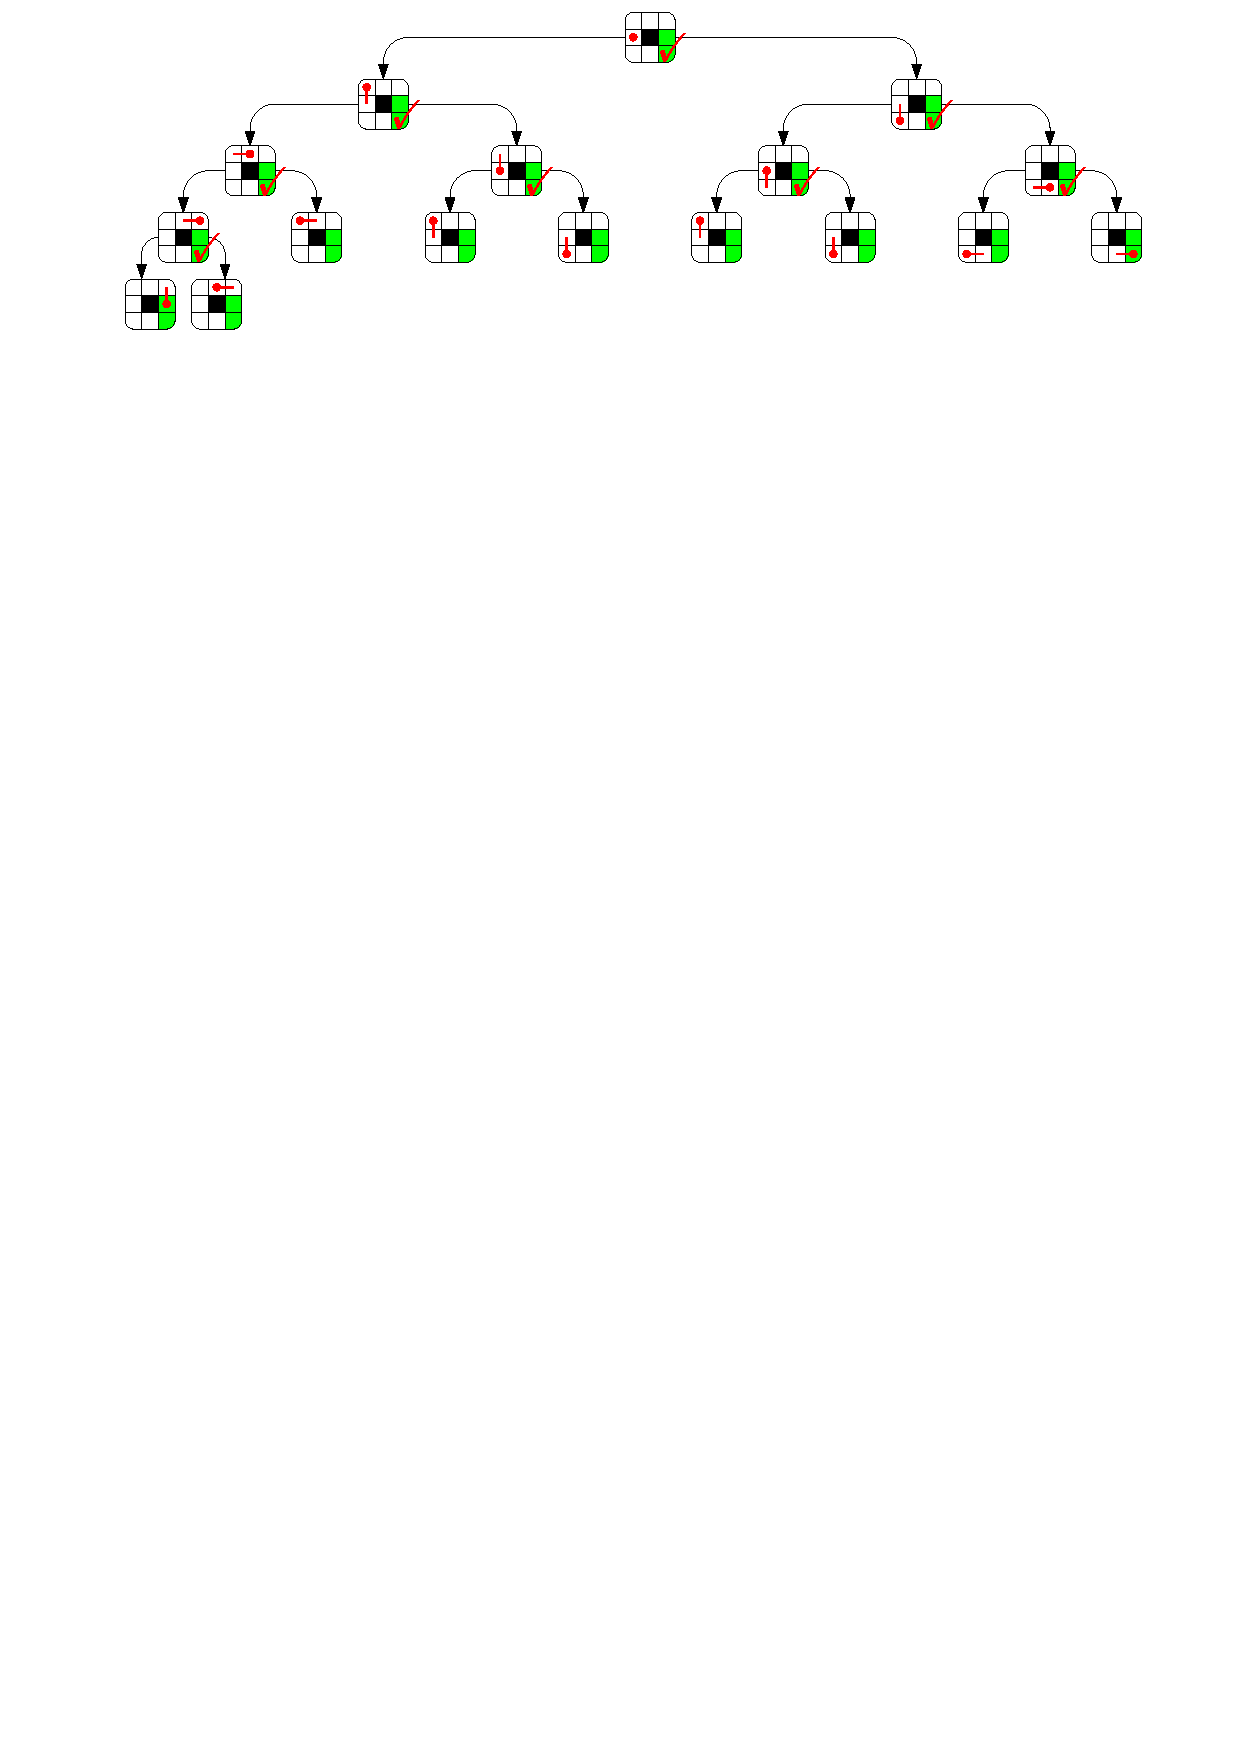
\includegraphics[width=\linewidth]{figs/bfs7.pdf}}%
  \only<10>{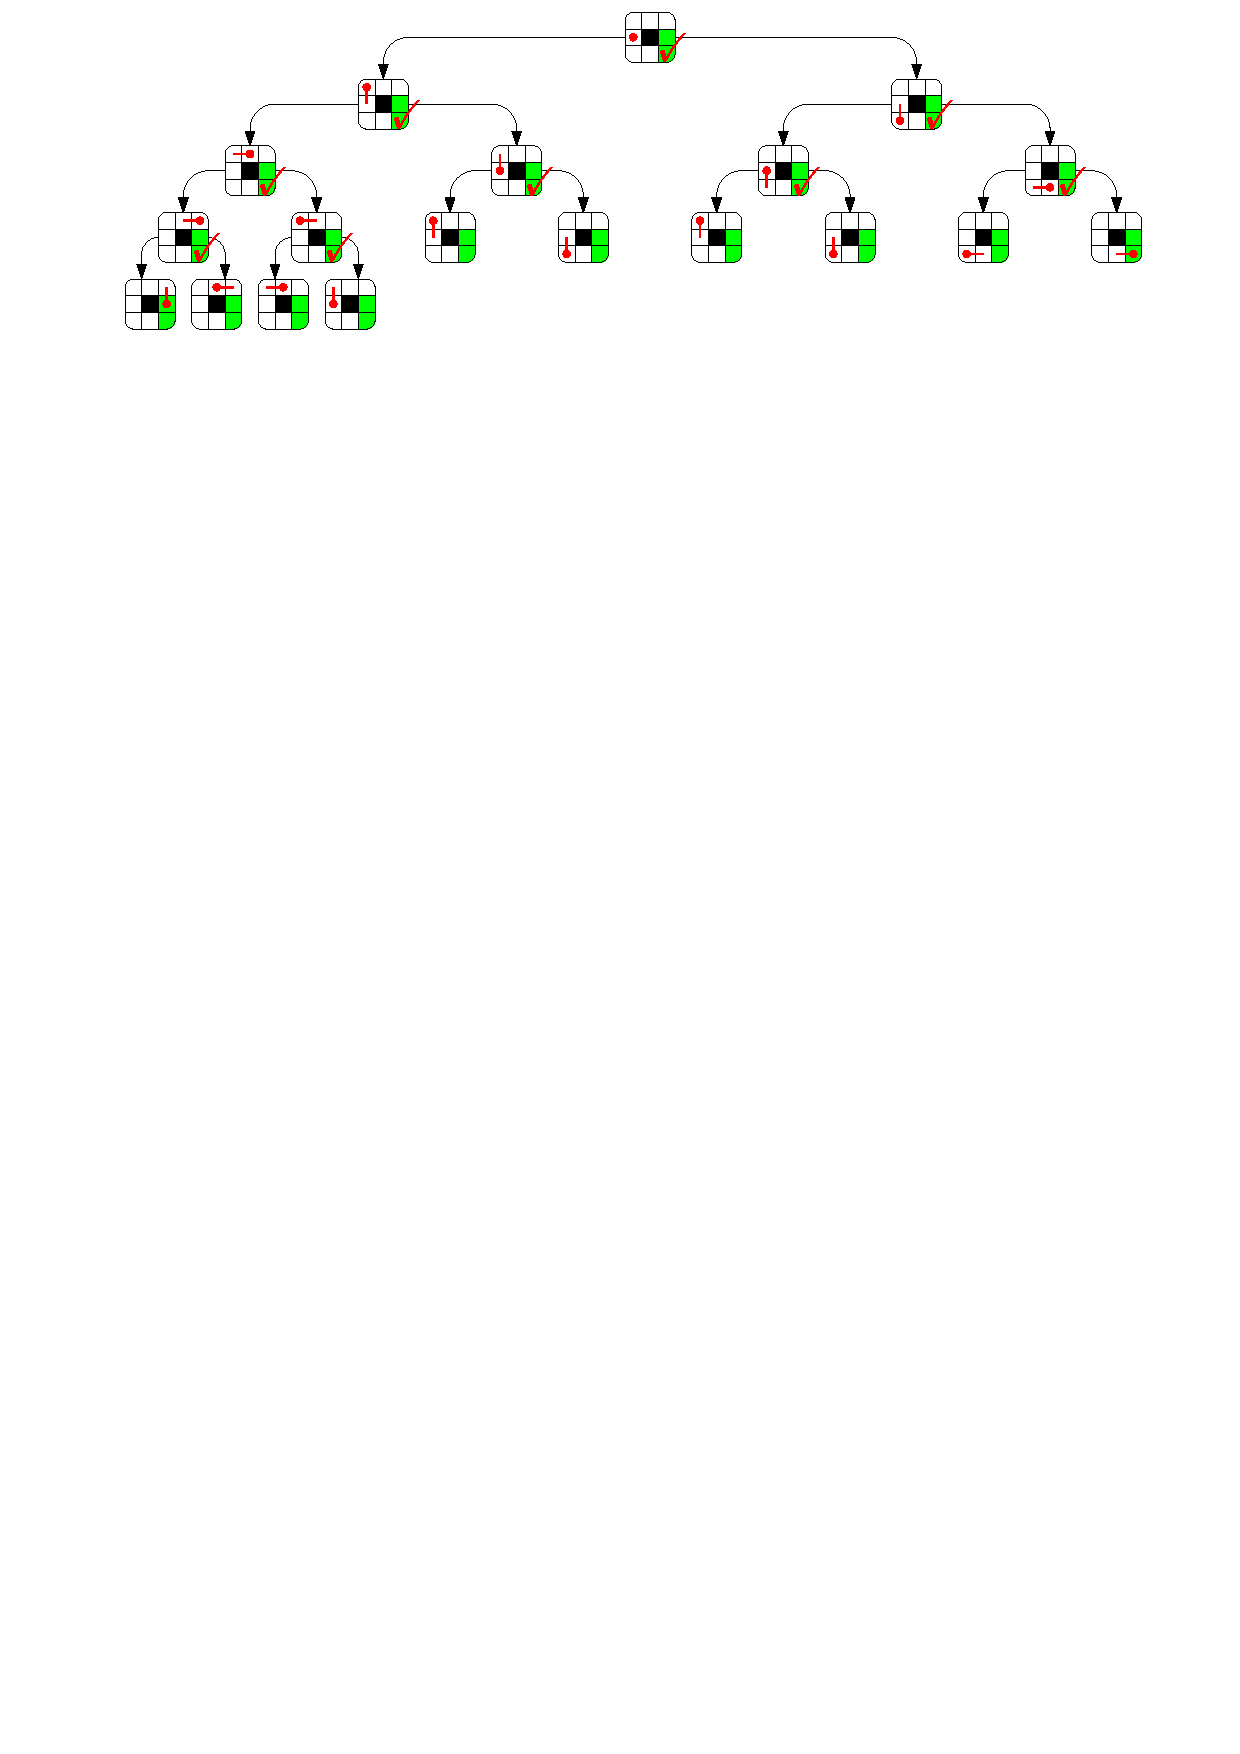
\includegraphics[width=\linewidth]{figs/bfs6.pdf}}%
  \only<11>{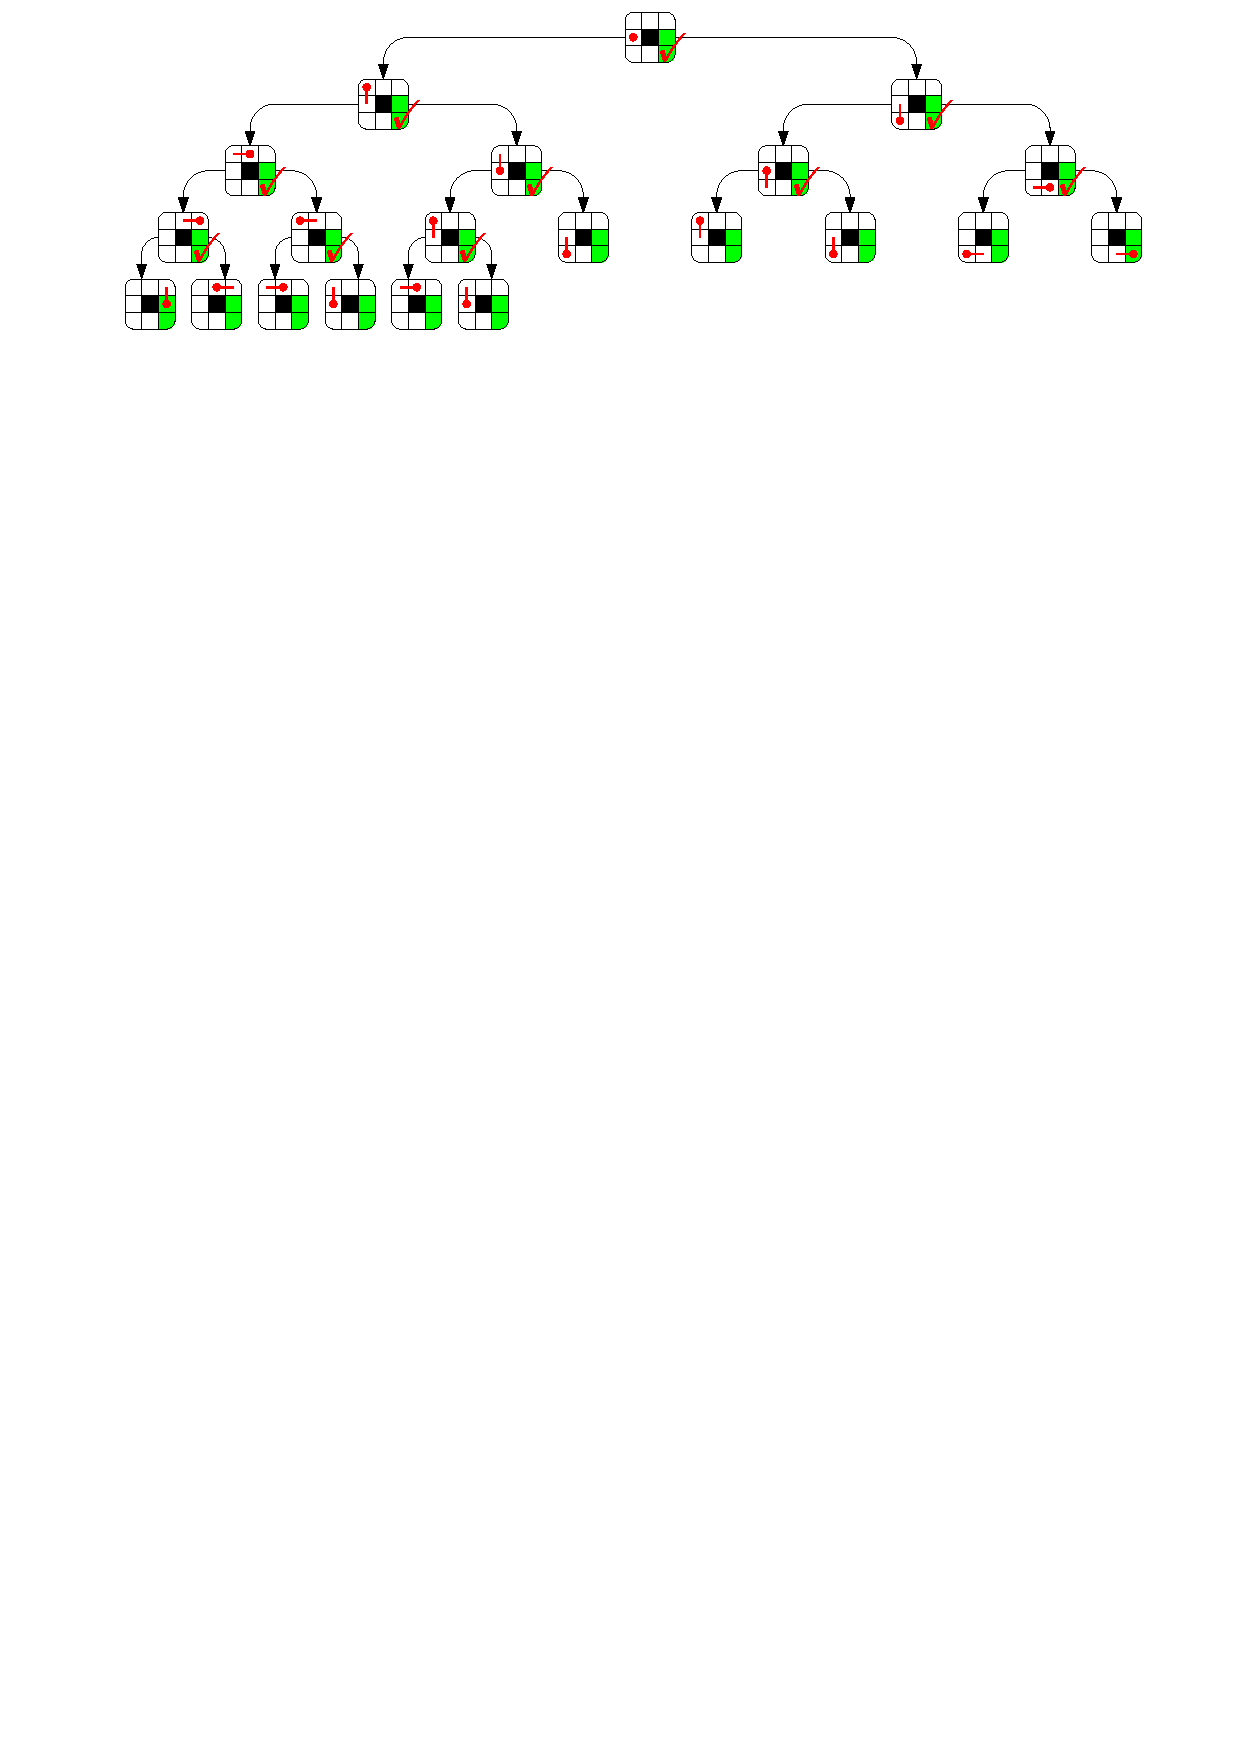
\includegraphics[width=\linewidth]{figs/bfs5.pdf}}%
  \only<12>{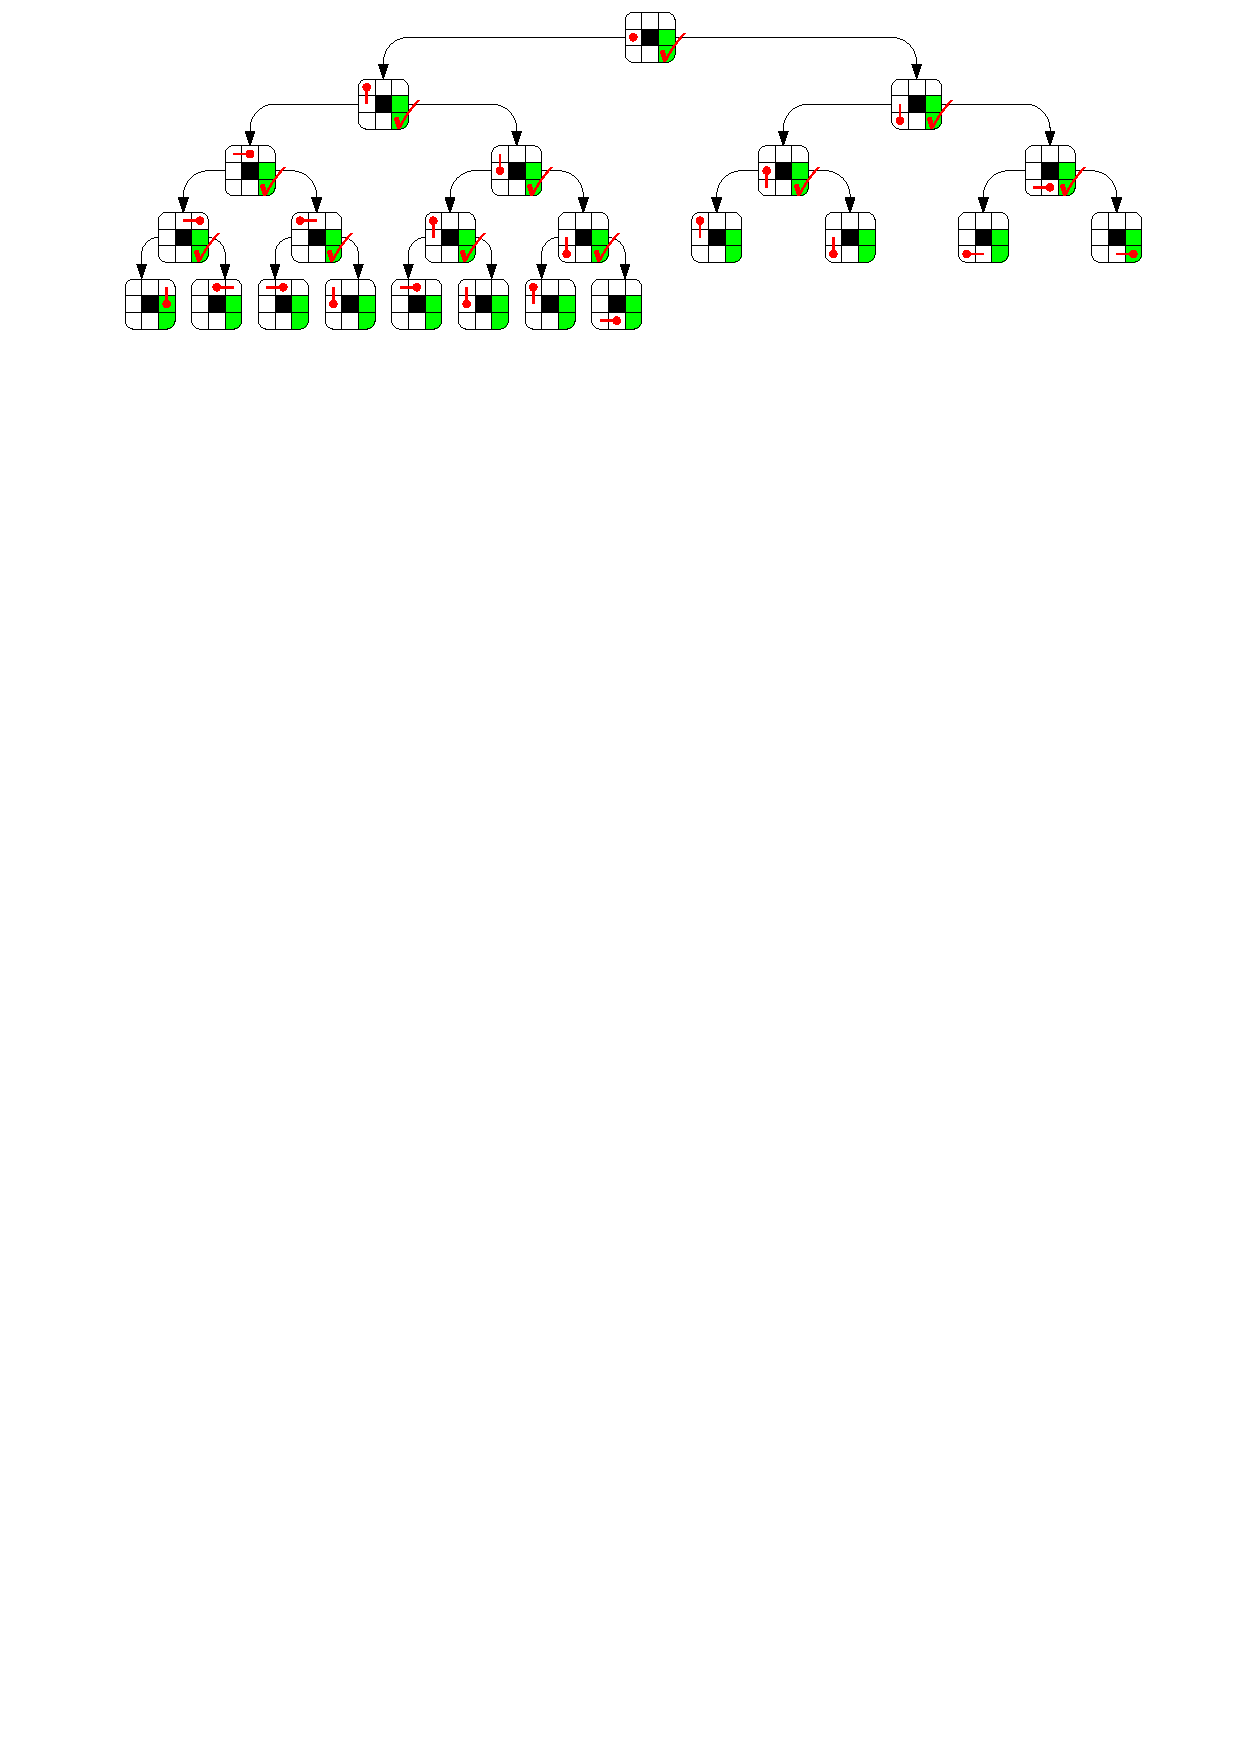
\includegraphics[width=\linewidth]{figs/bfs4.pdf}}%
  \only<13>{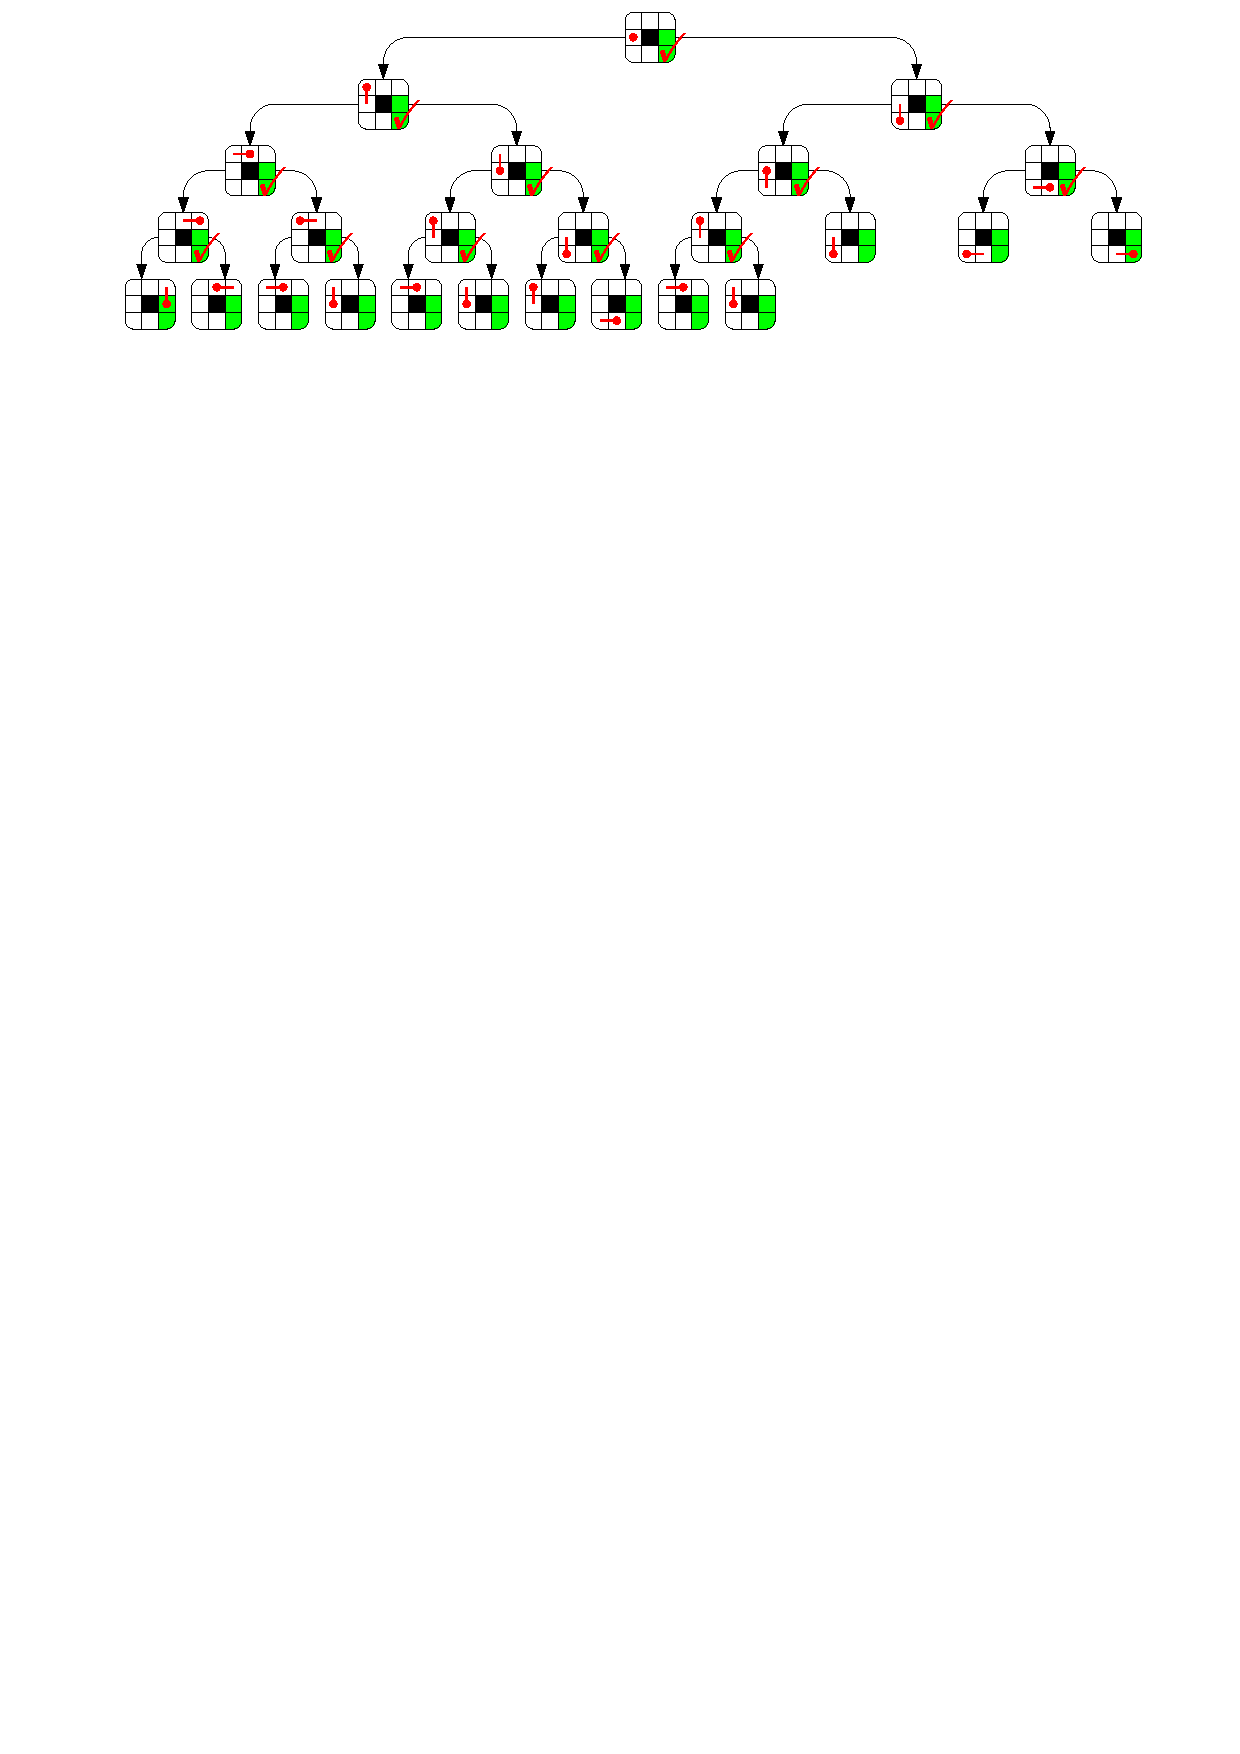
\includegraphics[width=\linewidth]{figs/bfs3.pdf}}%
  \only<14>{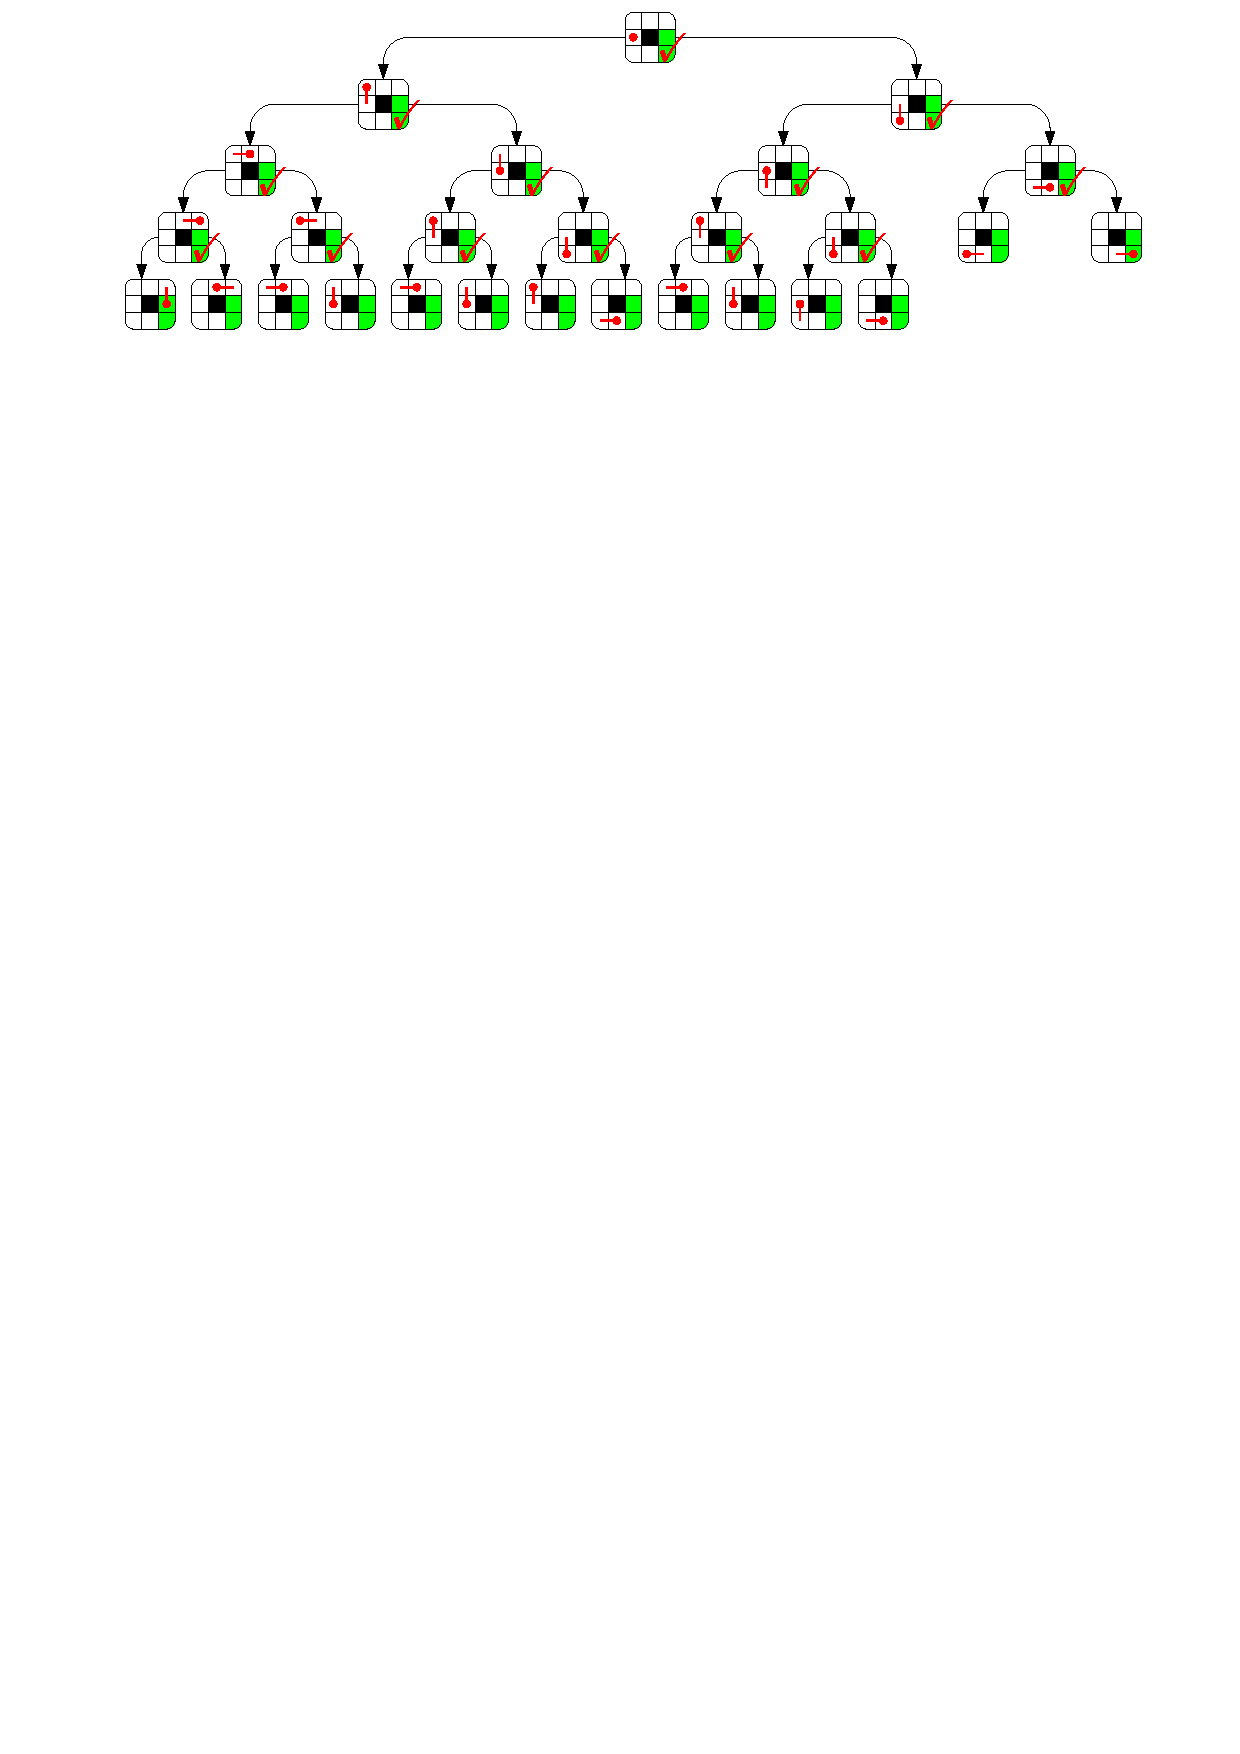
\includegraphics[width=\linewidth]{figs/bfs2.pdf}}%
  \only<15>{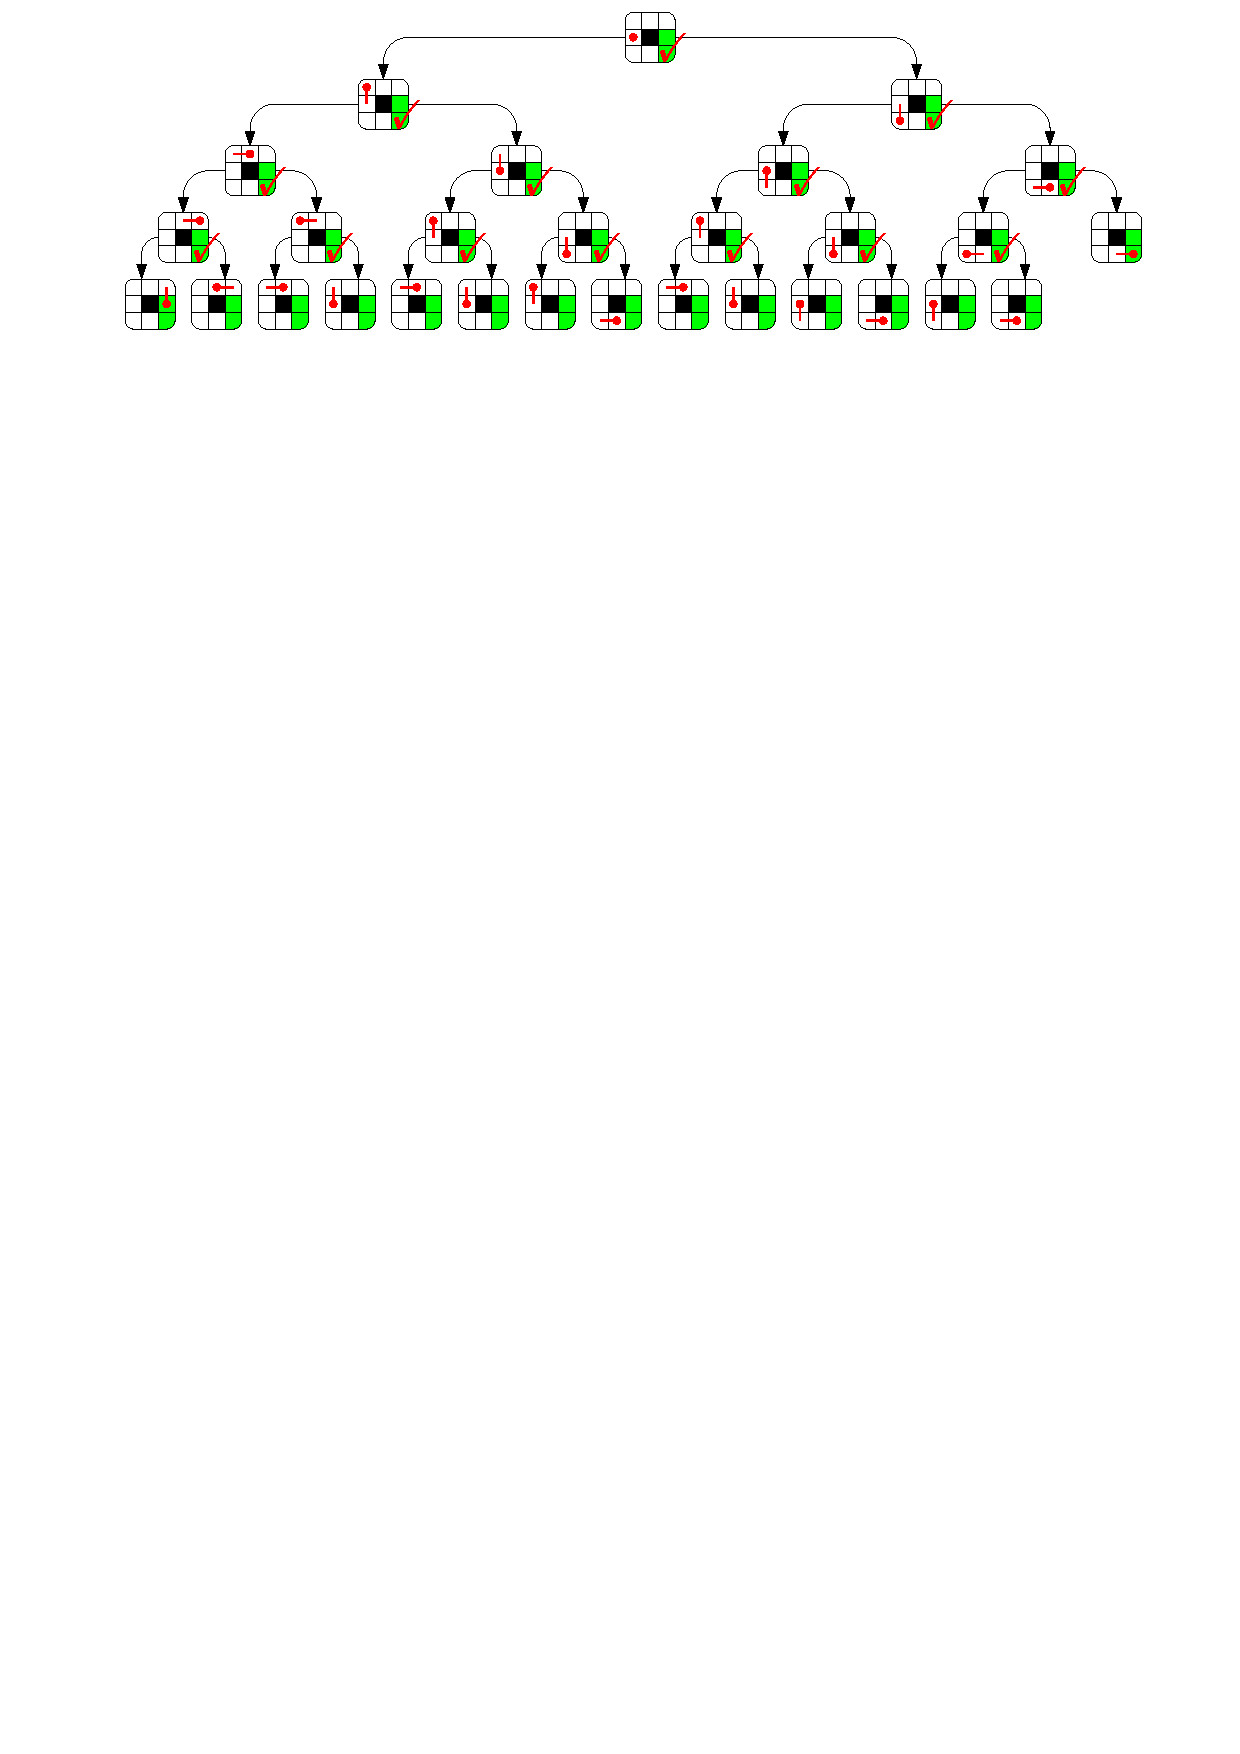
\includegraphics[width=\linewidth]{figs/bfs1.pdf}}%
  \only<16->{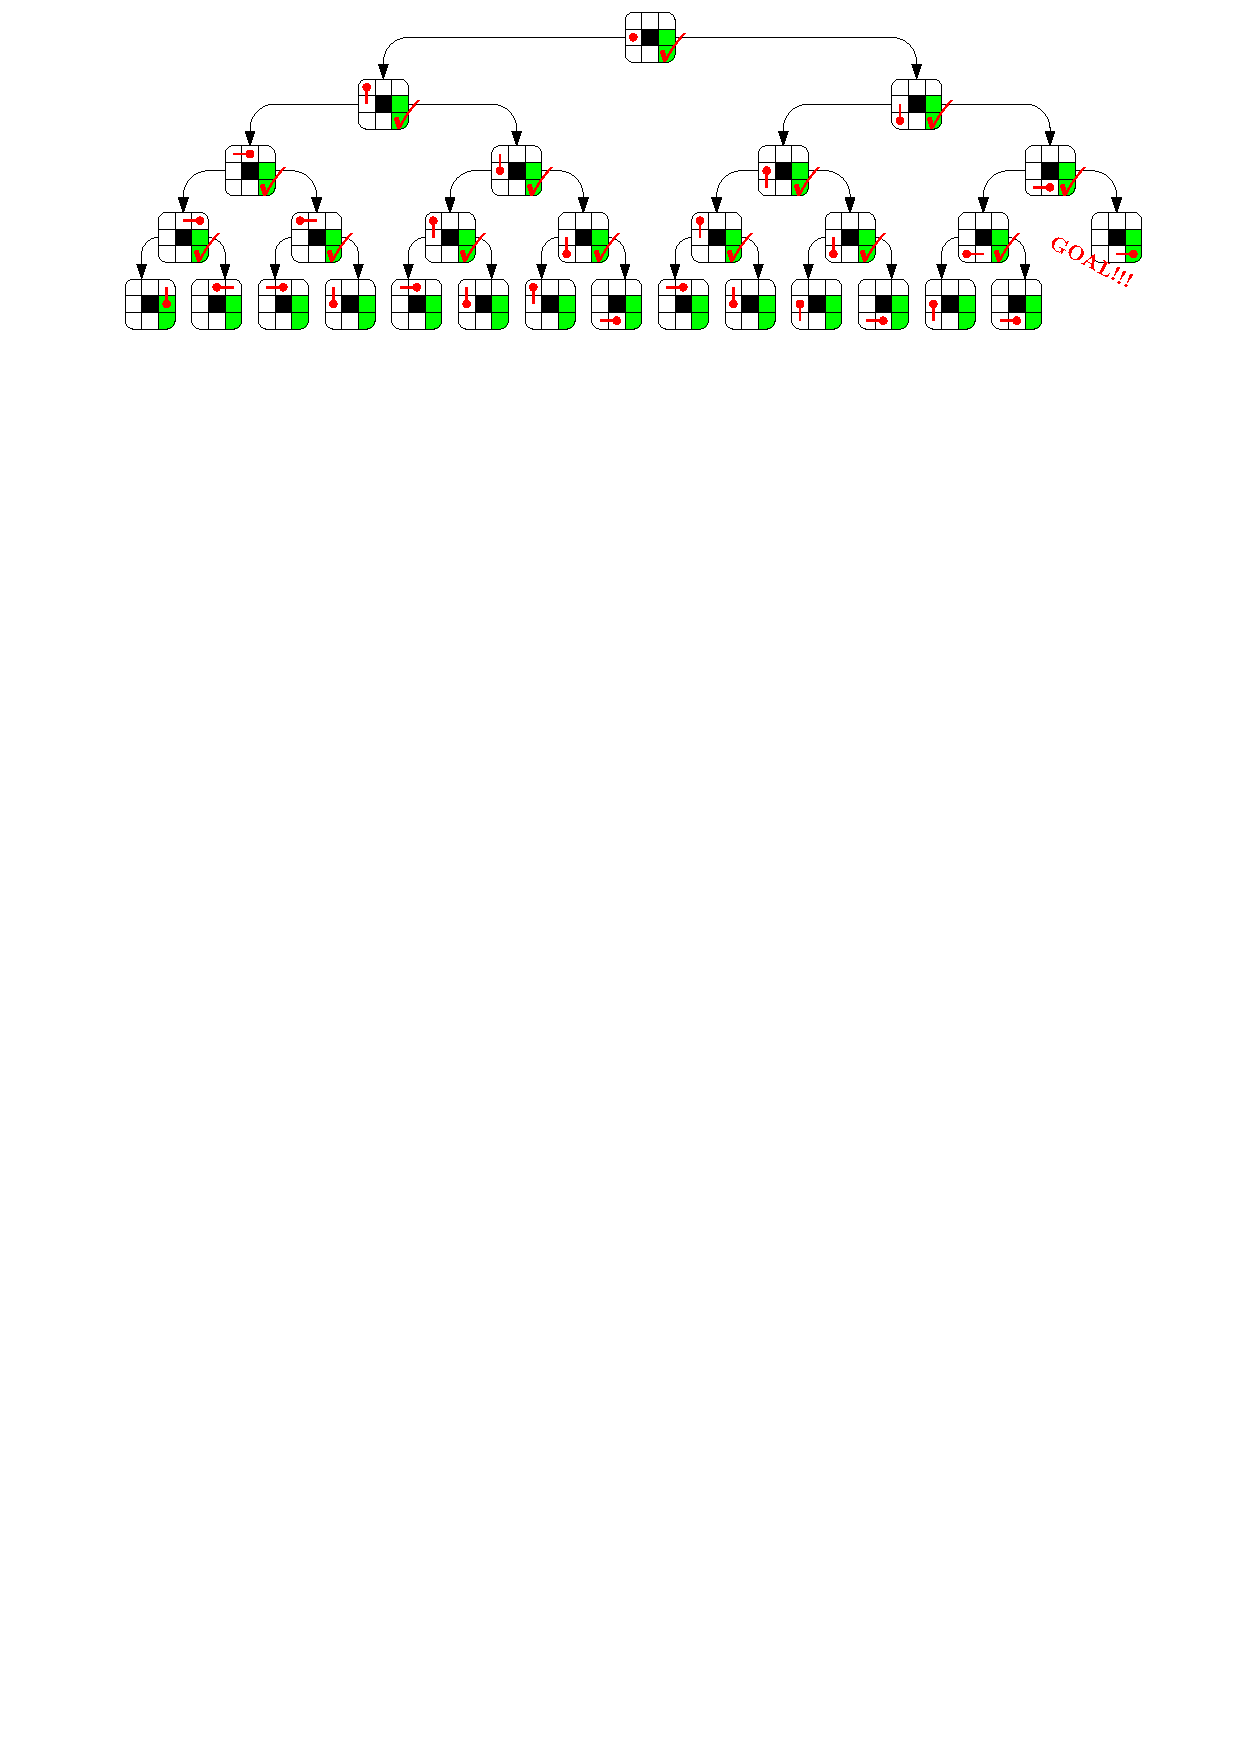
\includegraphics[width=\linewidth]{figs/bfs0.pdf}}%

  \only<17>{
    \begin{center}
      \Large Optimální, ale (potenciálně) s exponenciální pamětí!
    \end{center}
  }
\end{frame}

\begin{frame}[t]
  \frametitle{Prohledávání do hloubky (DFS)}

  \vspace{3em}

  \only<1>{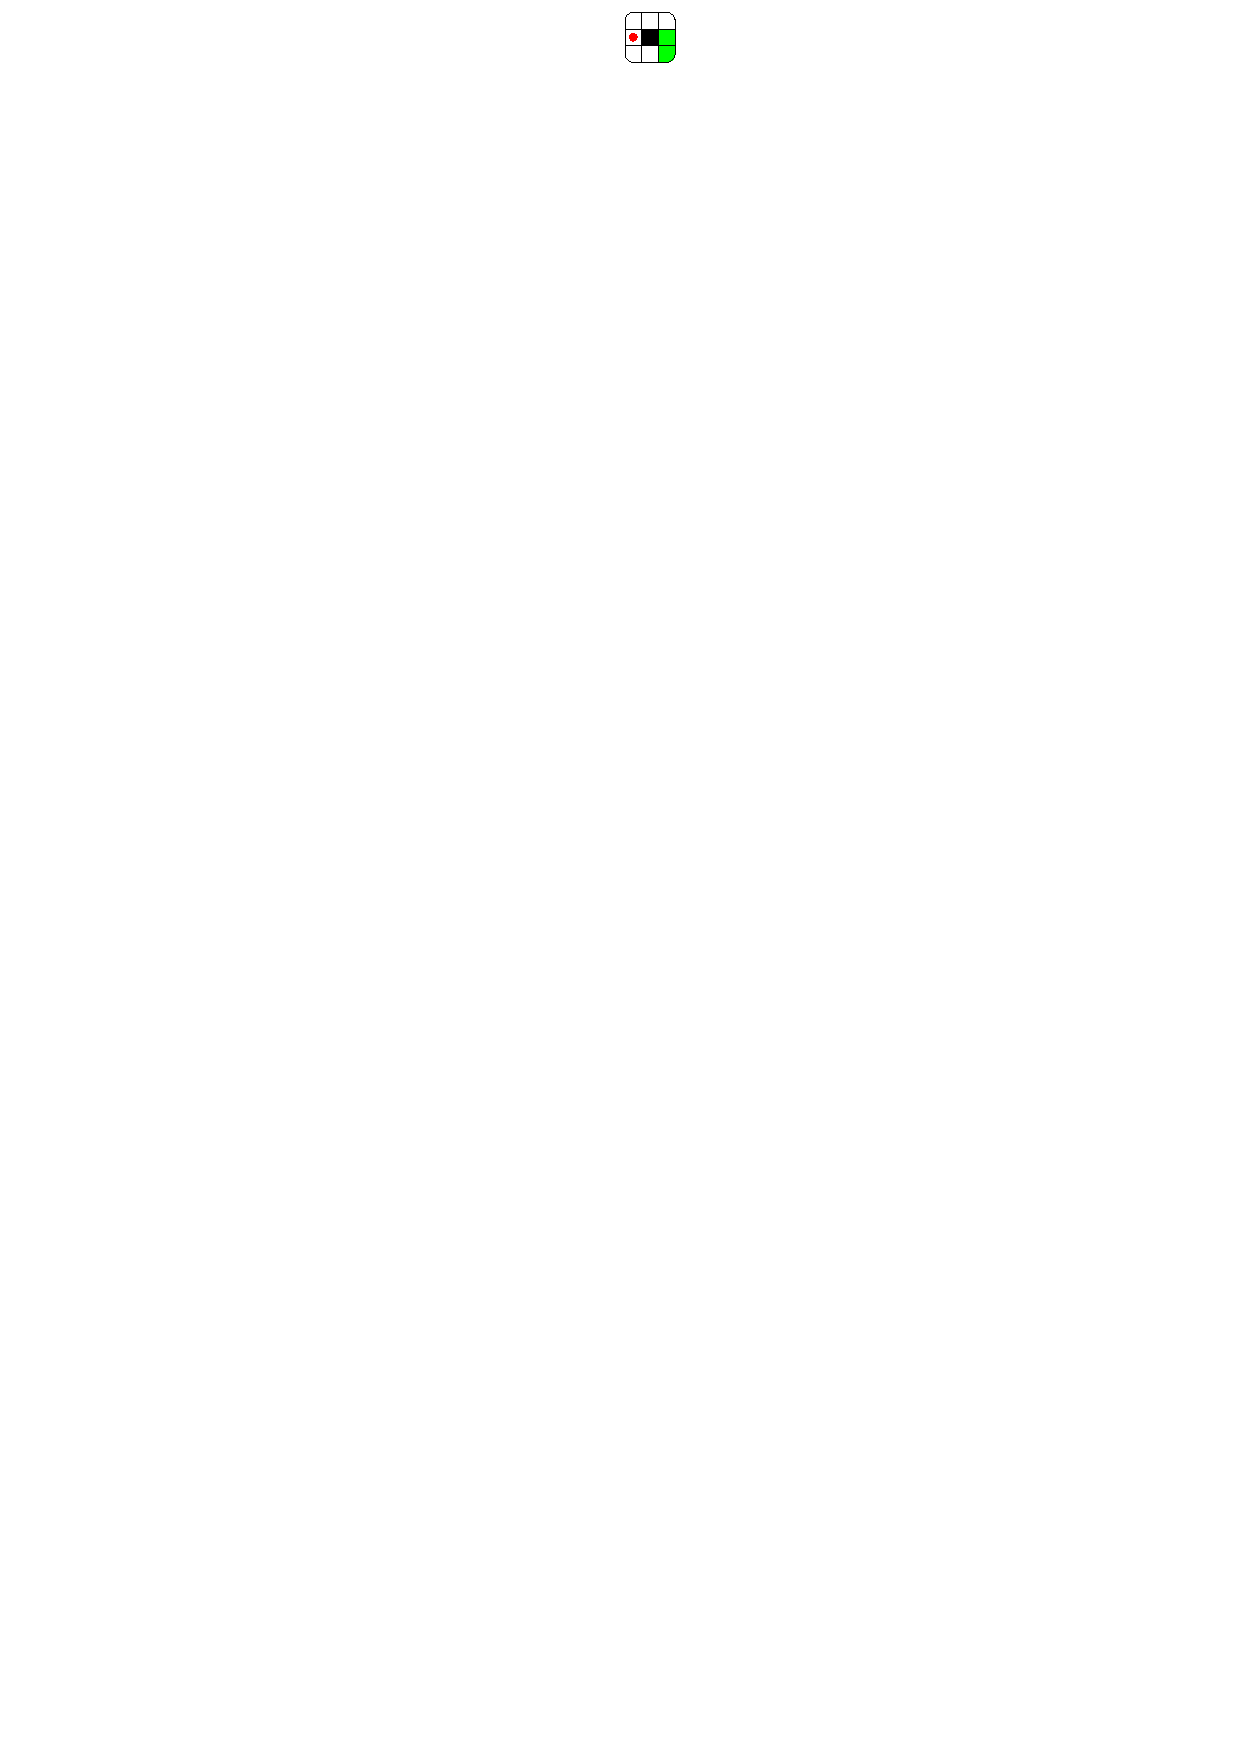
\includegraphics[width=\linewidth]{figs/dfs6.pdf}}%
  \only<2>{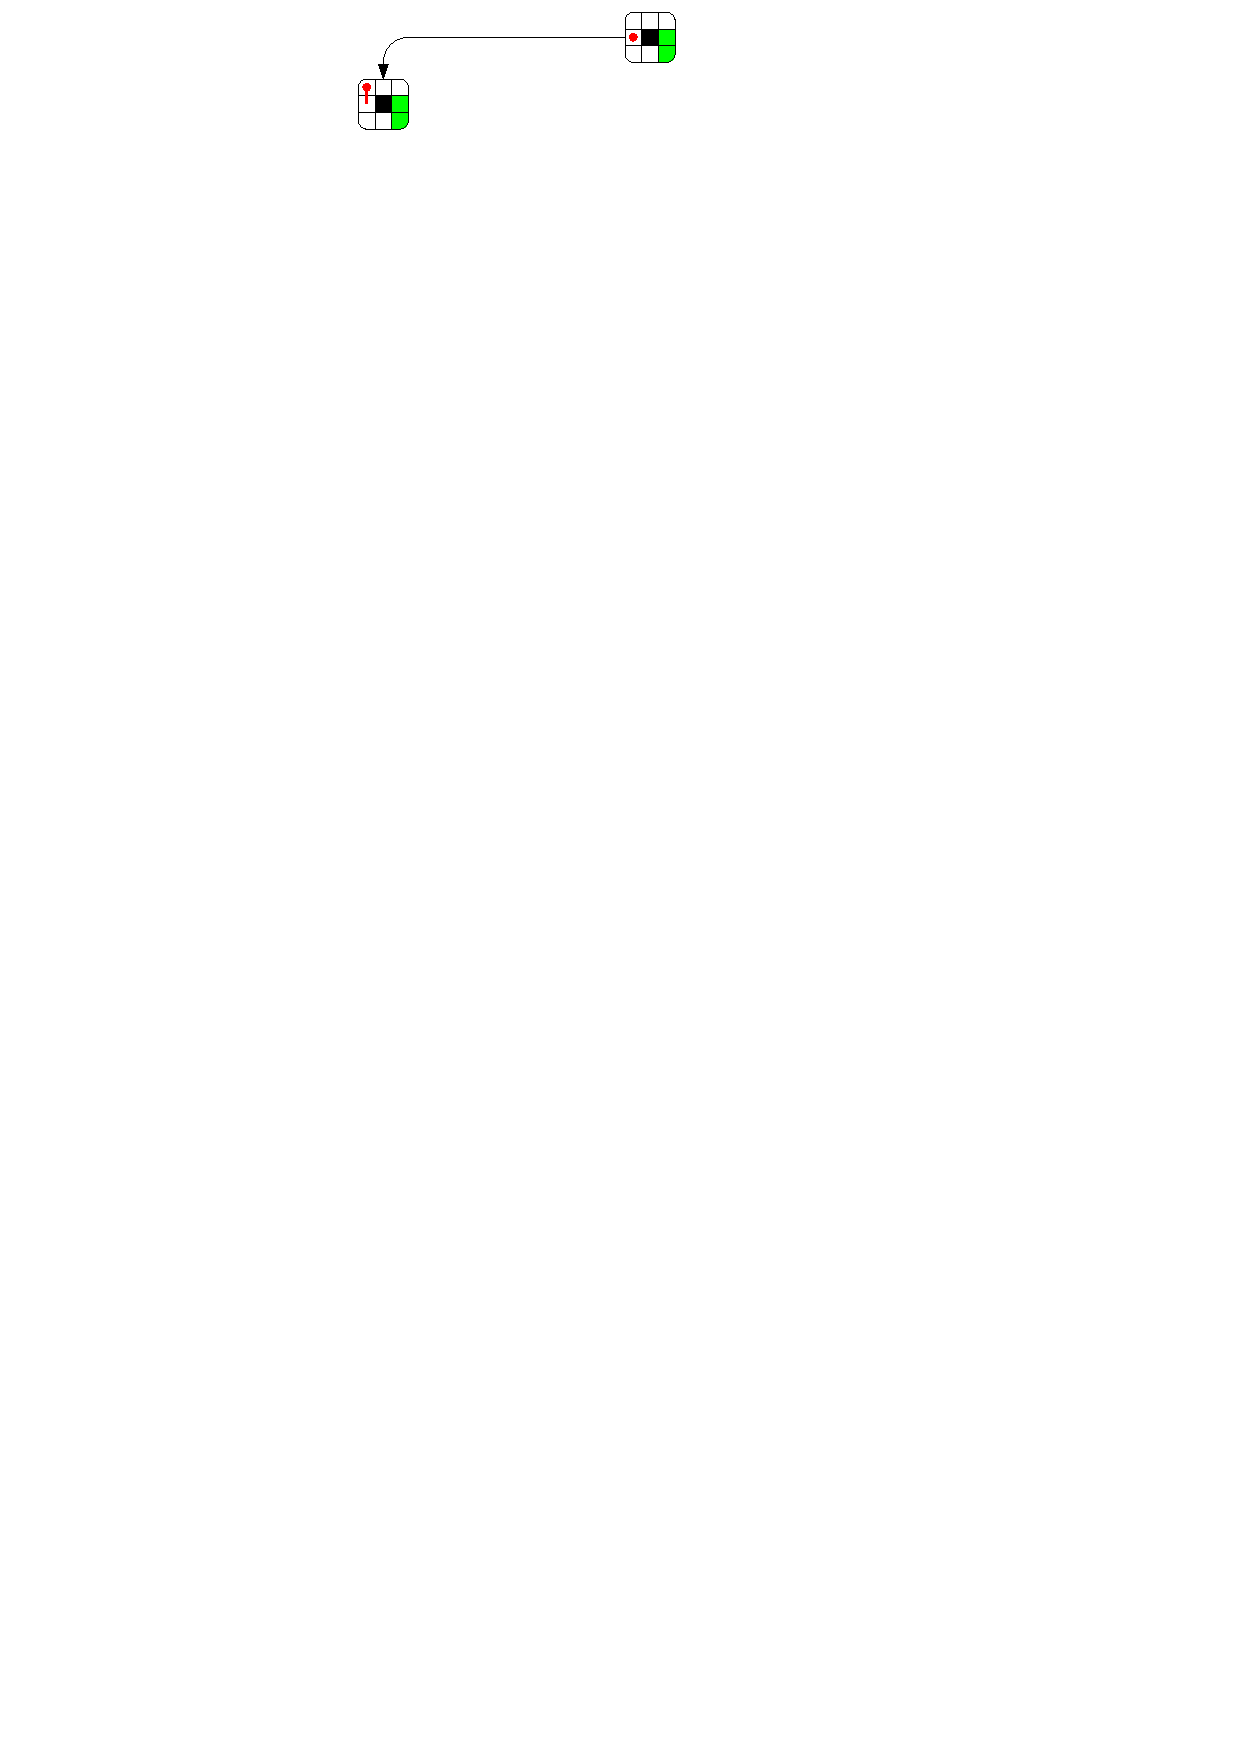
\includegraphics[width=\linewidth]{figs/dfs5.pdf}}%
  \only<3>{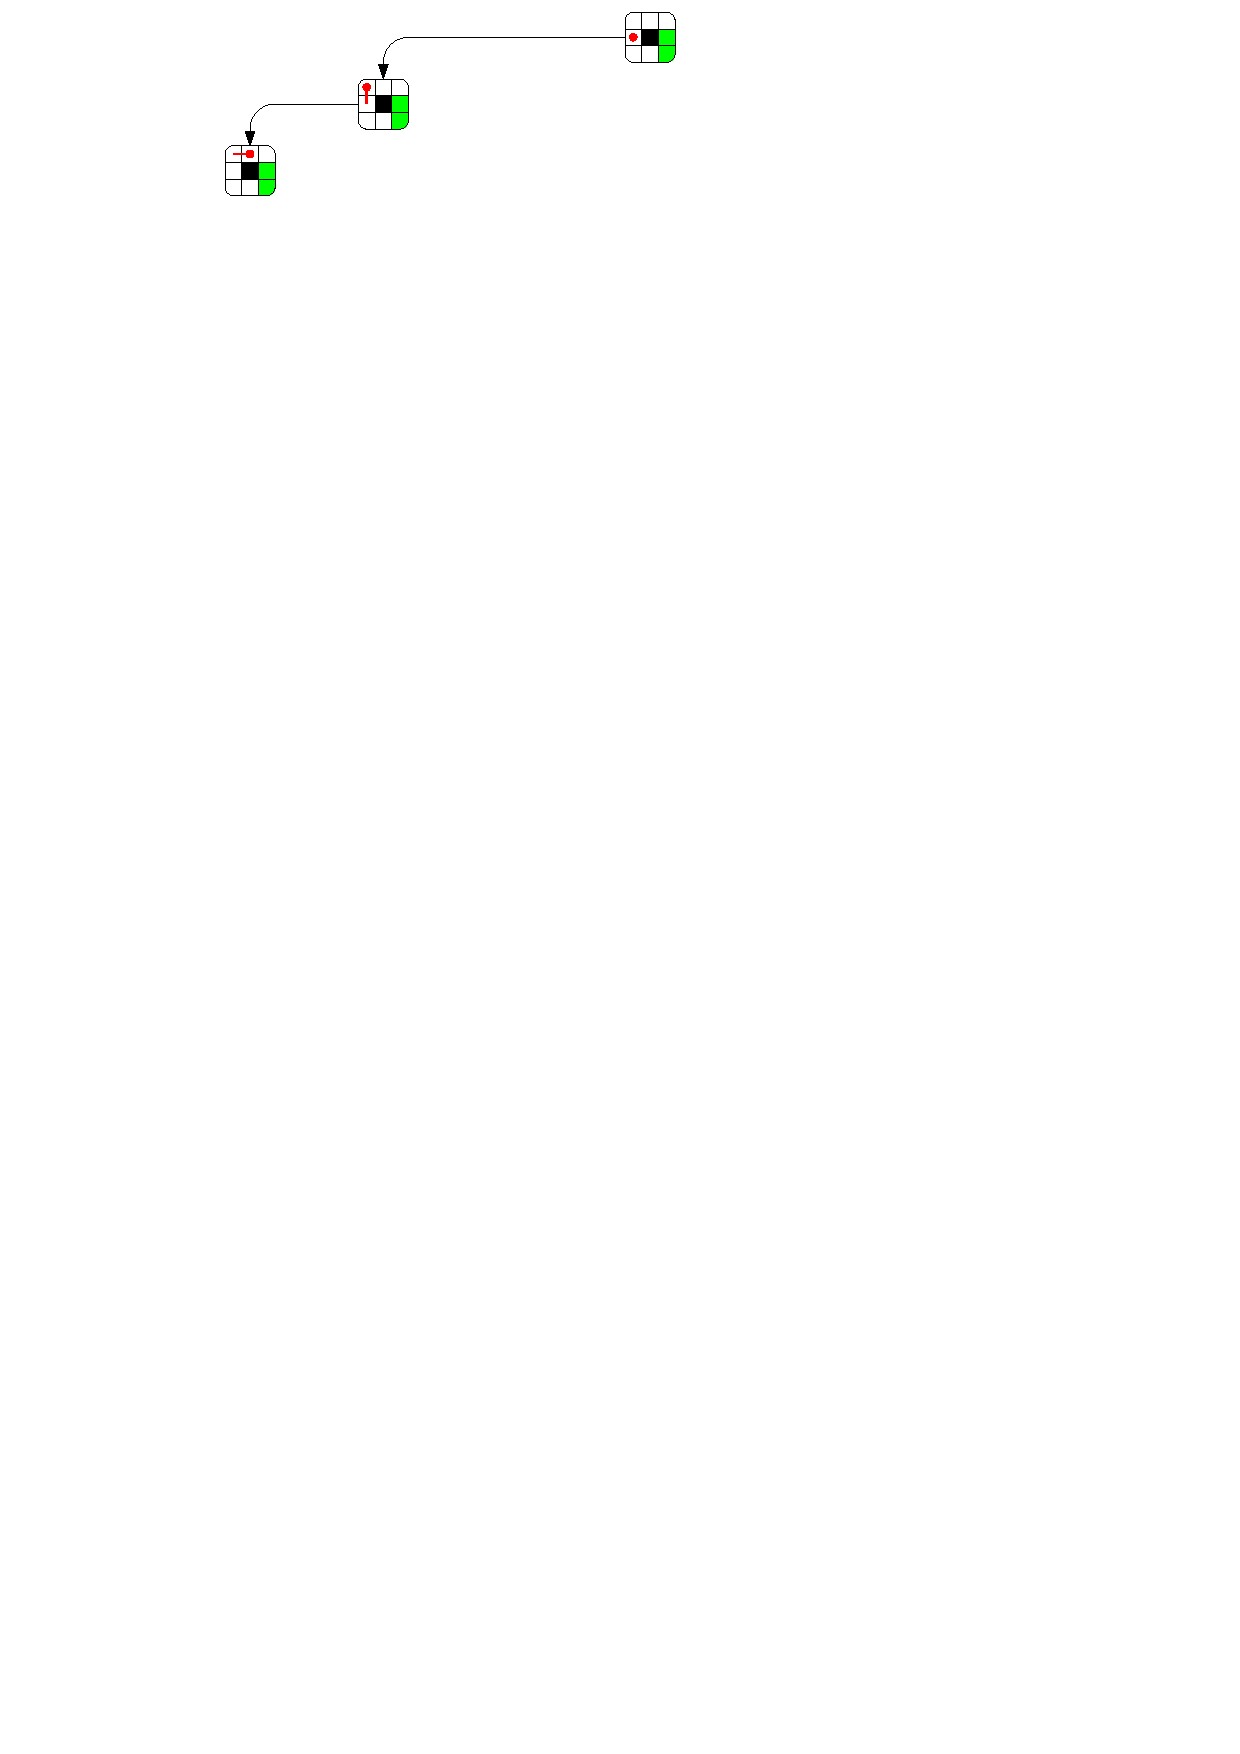
\includegraphics[width=\linewidth]{figs/dfs4.pdf}}%
  \only<4>{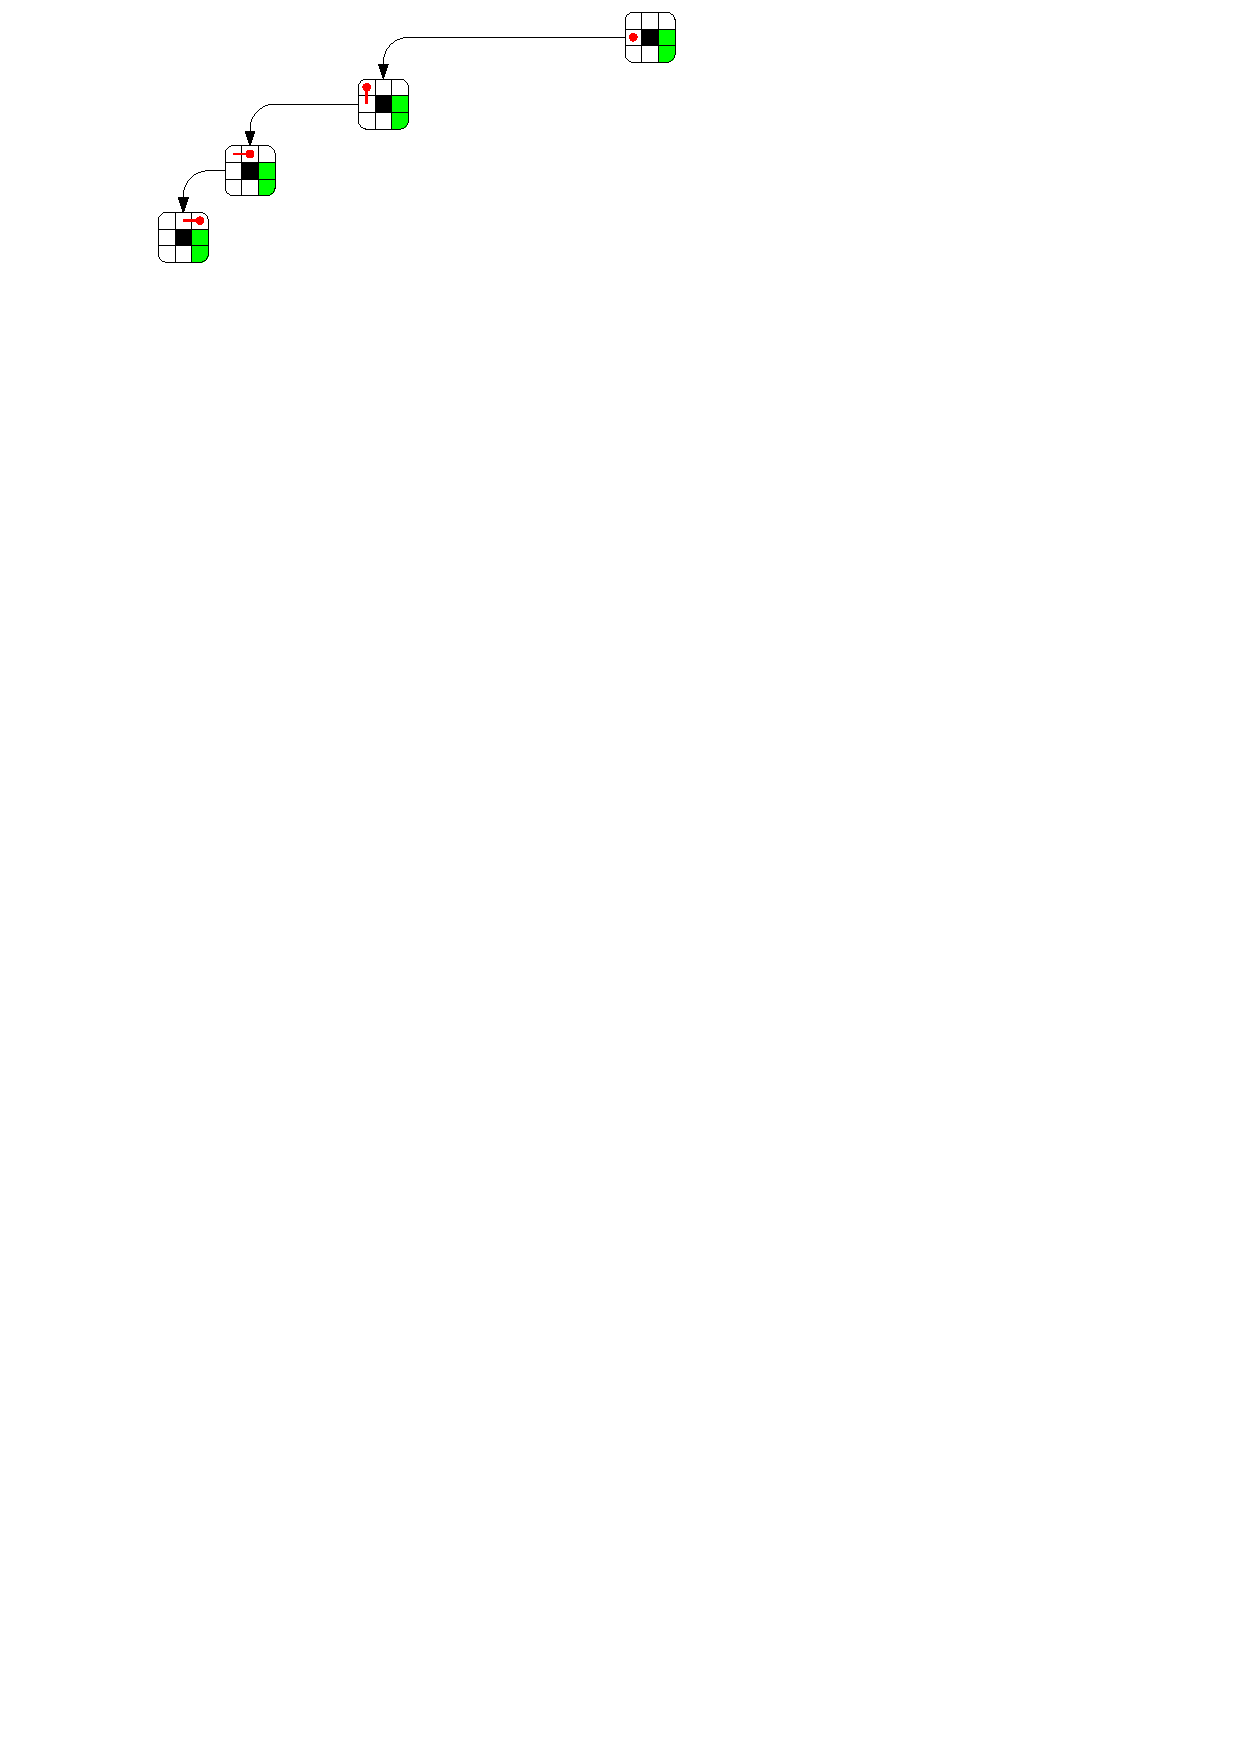
\includegraphics[width=\linewidth]{figs/dfs3.pdf}}%
  \only<5>{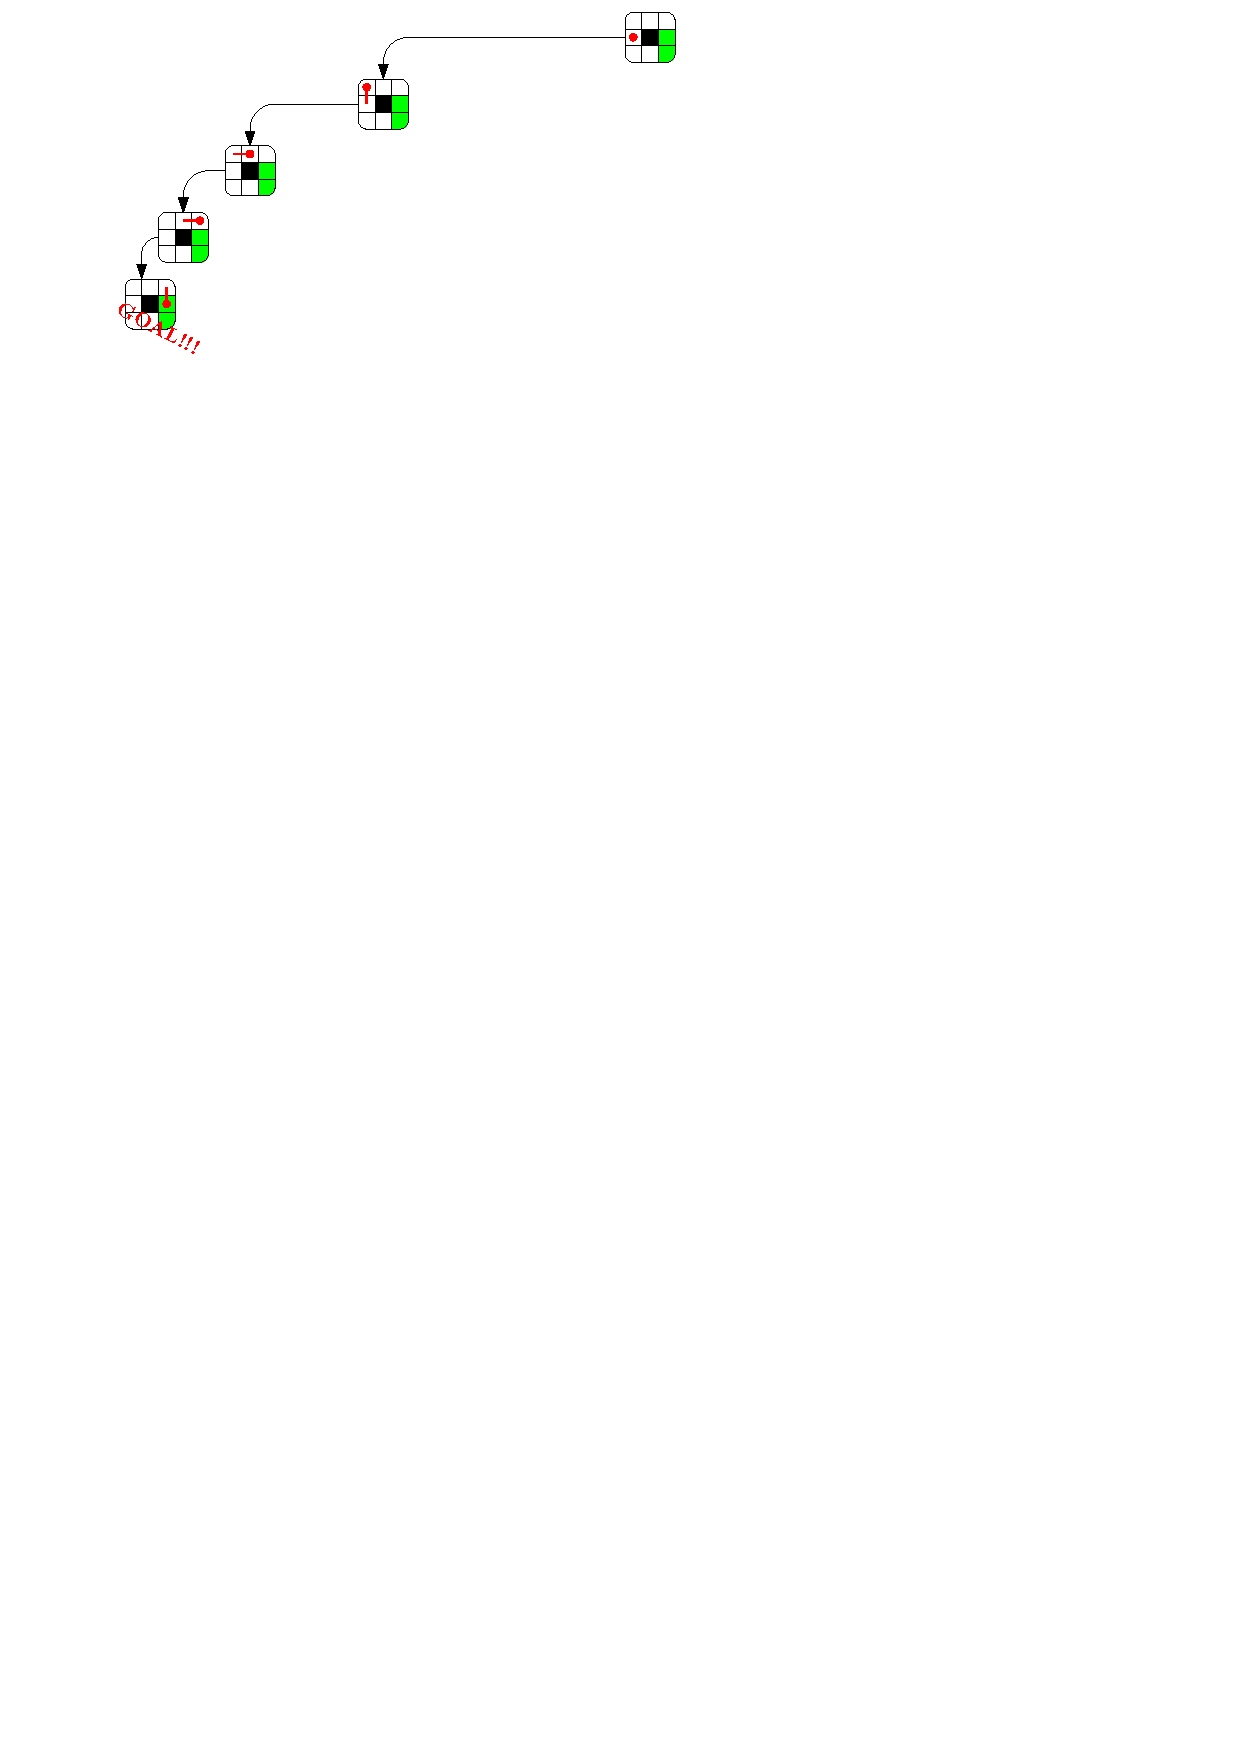
\includegraphics[width=\linewidth]{figs/dfs2.pdf}}%
  \only<6>{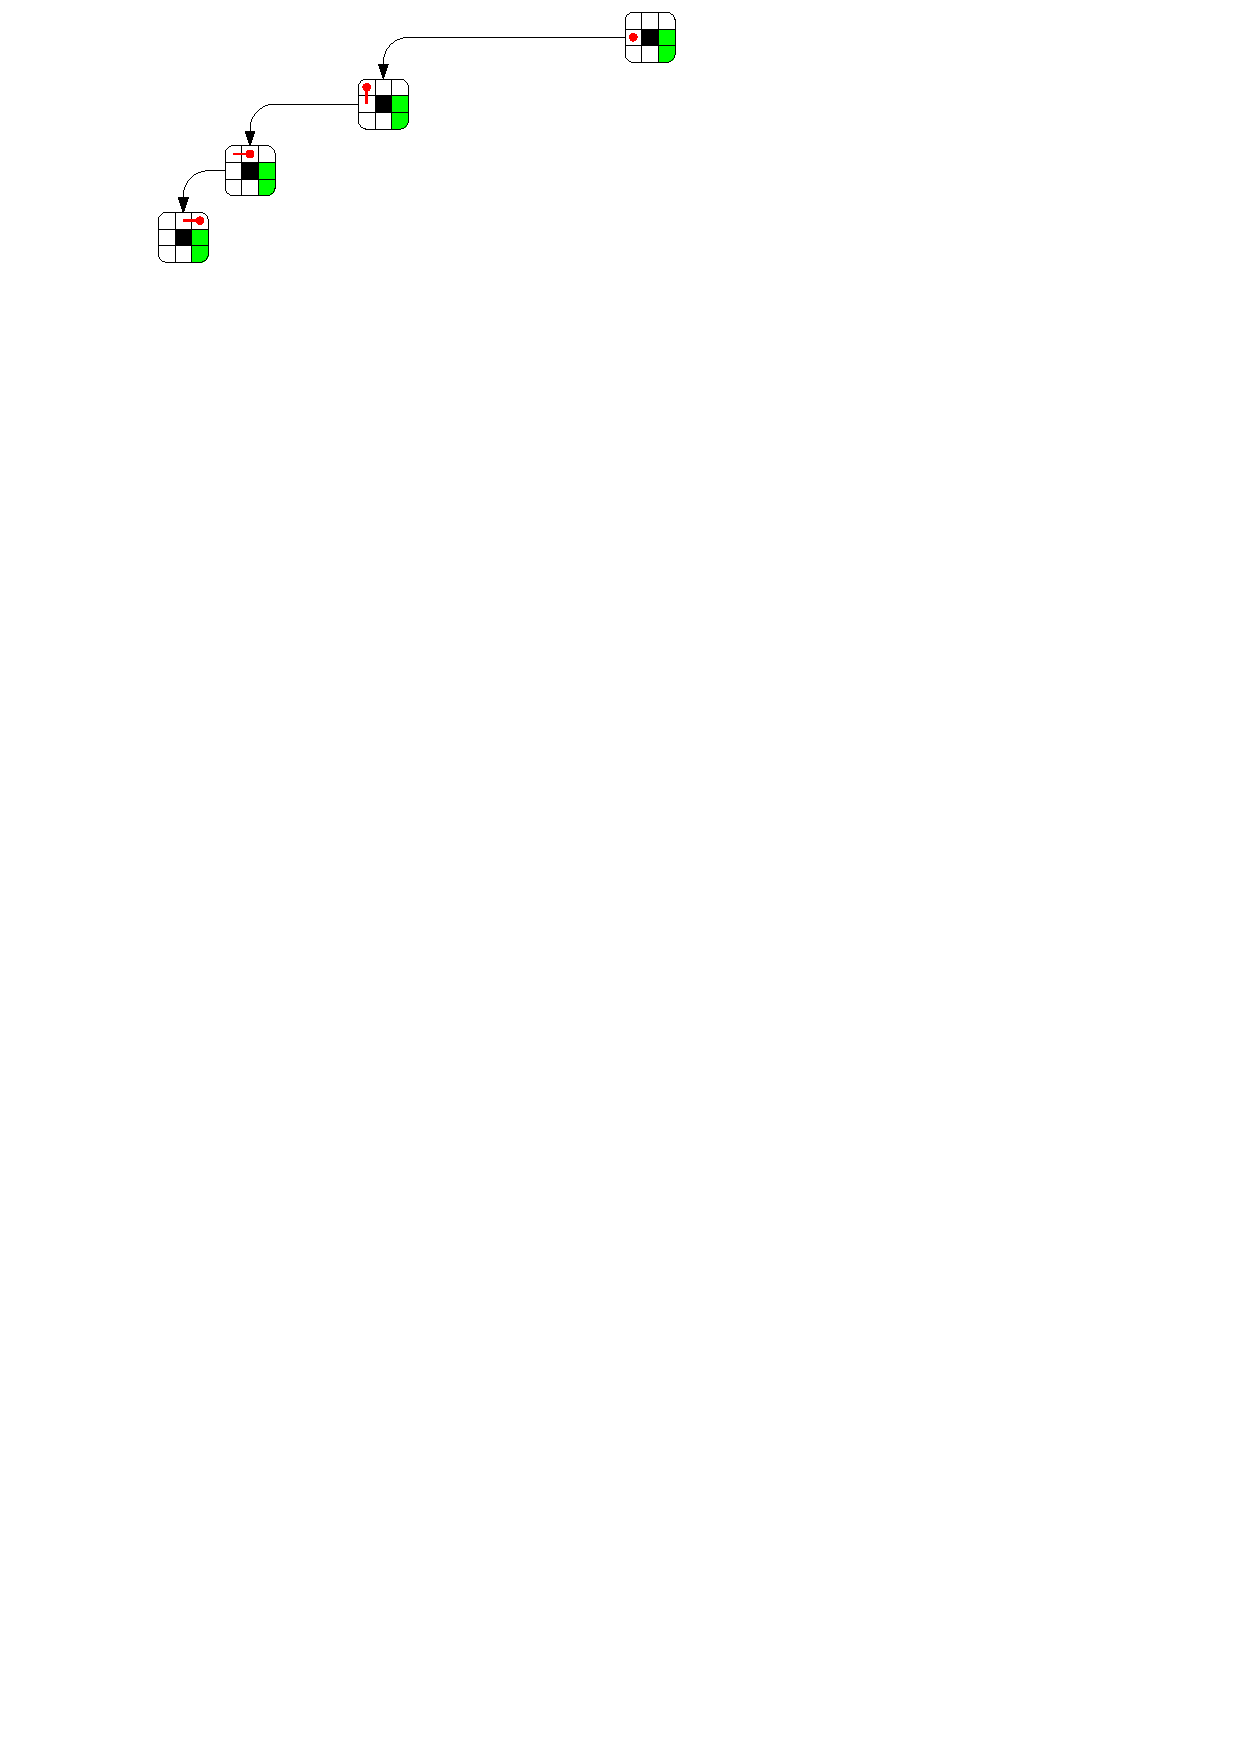
\includegraphics[width=\linewidth]{figs/dfs3.pdf}}%
  \only<7>{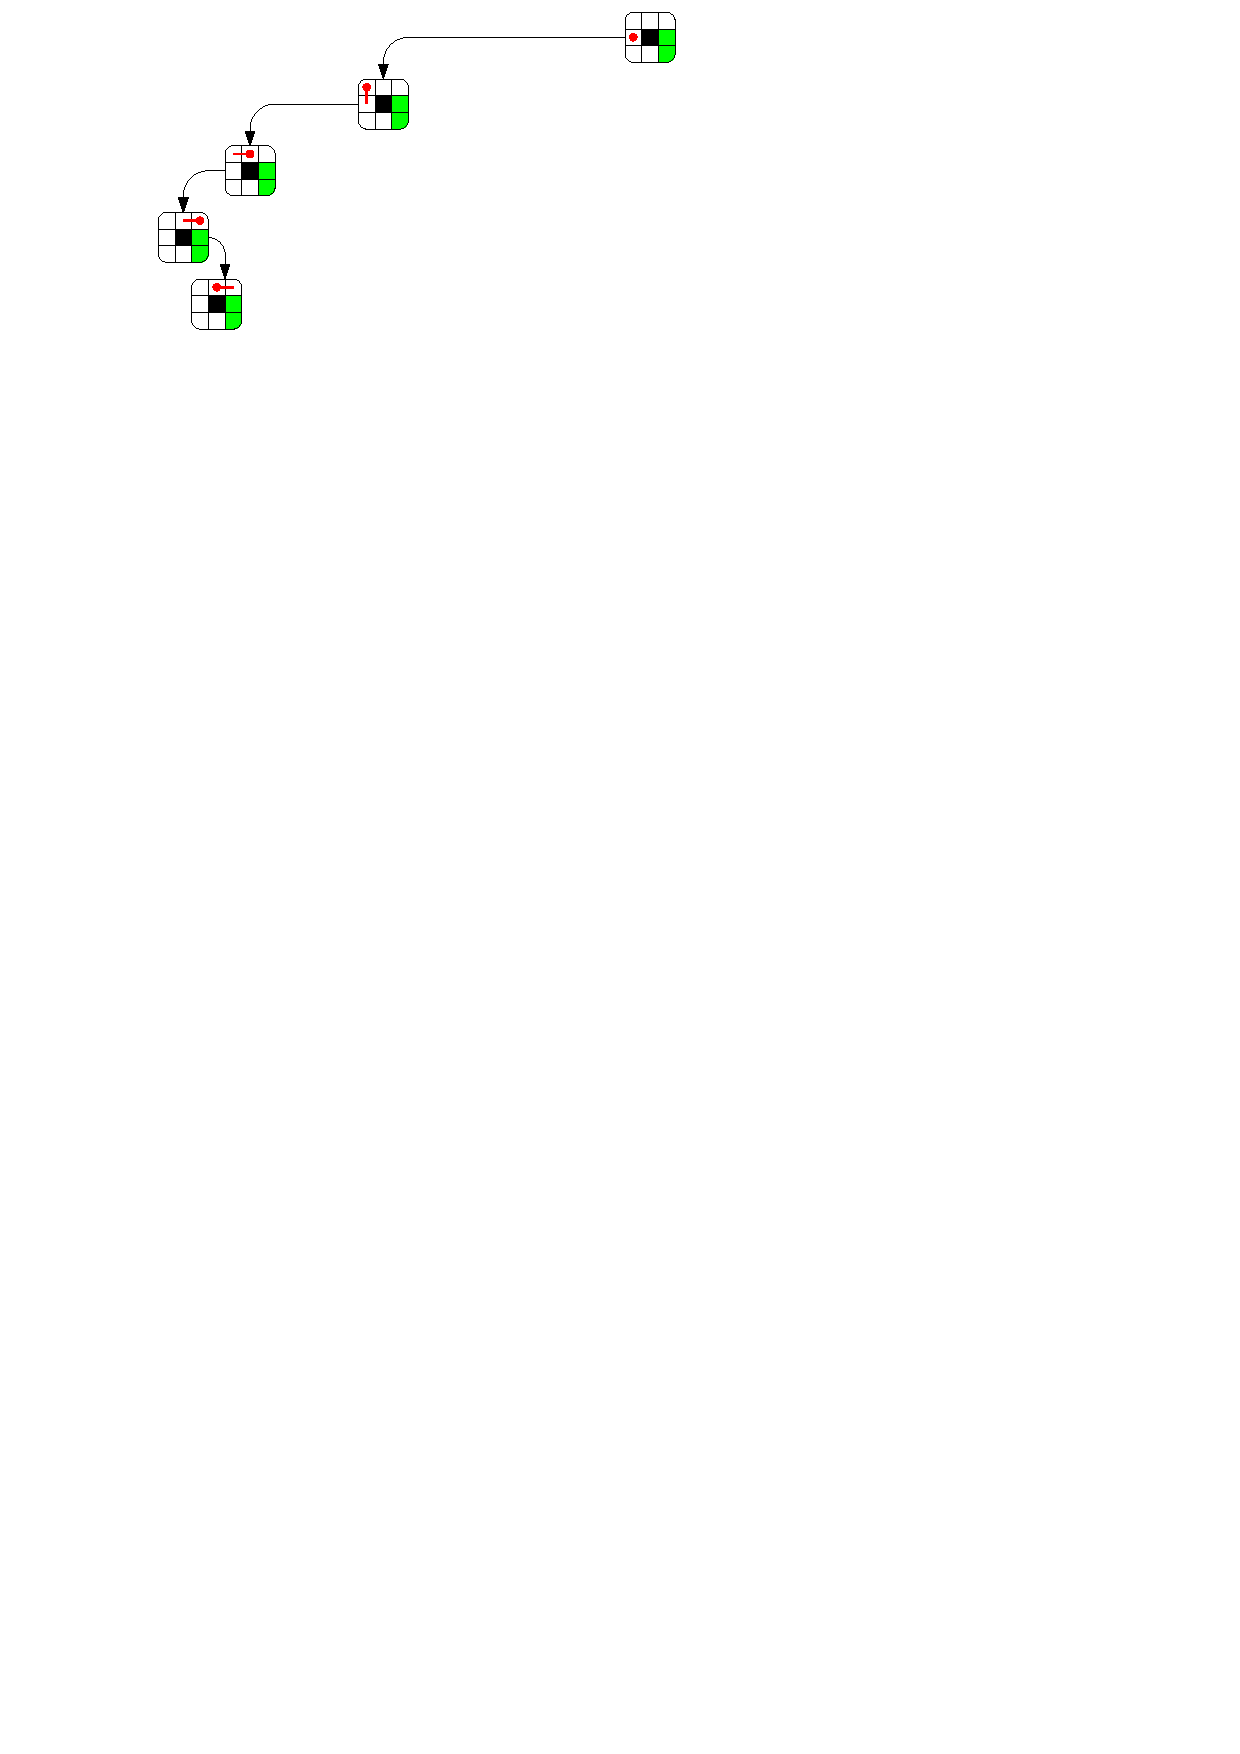
\includegraphics[width=\linewidth]{figs/dfs1.pdf}}%
  \only<8->{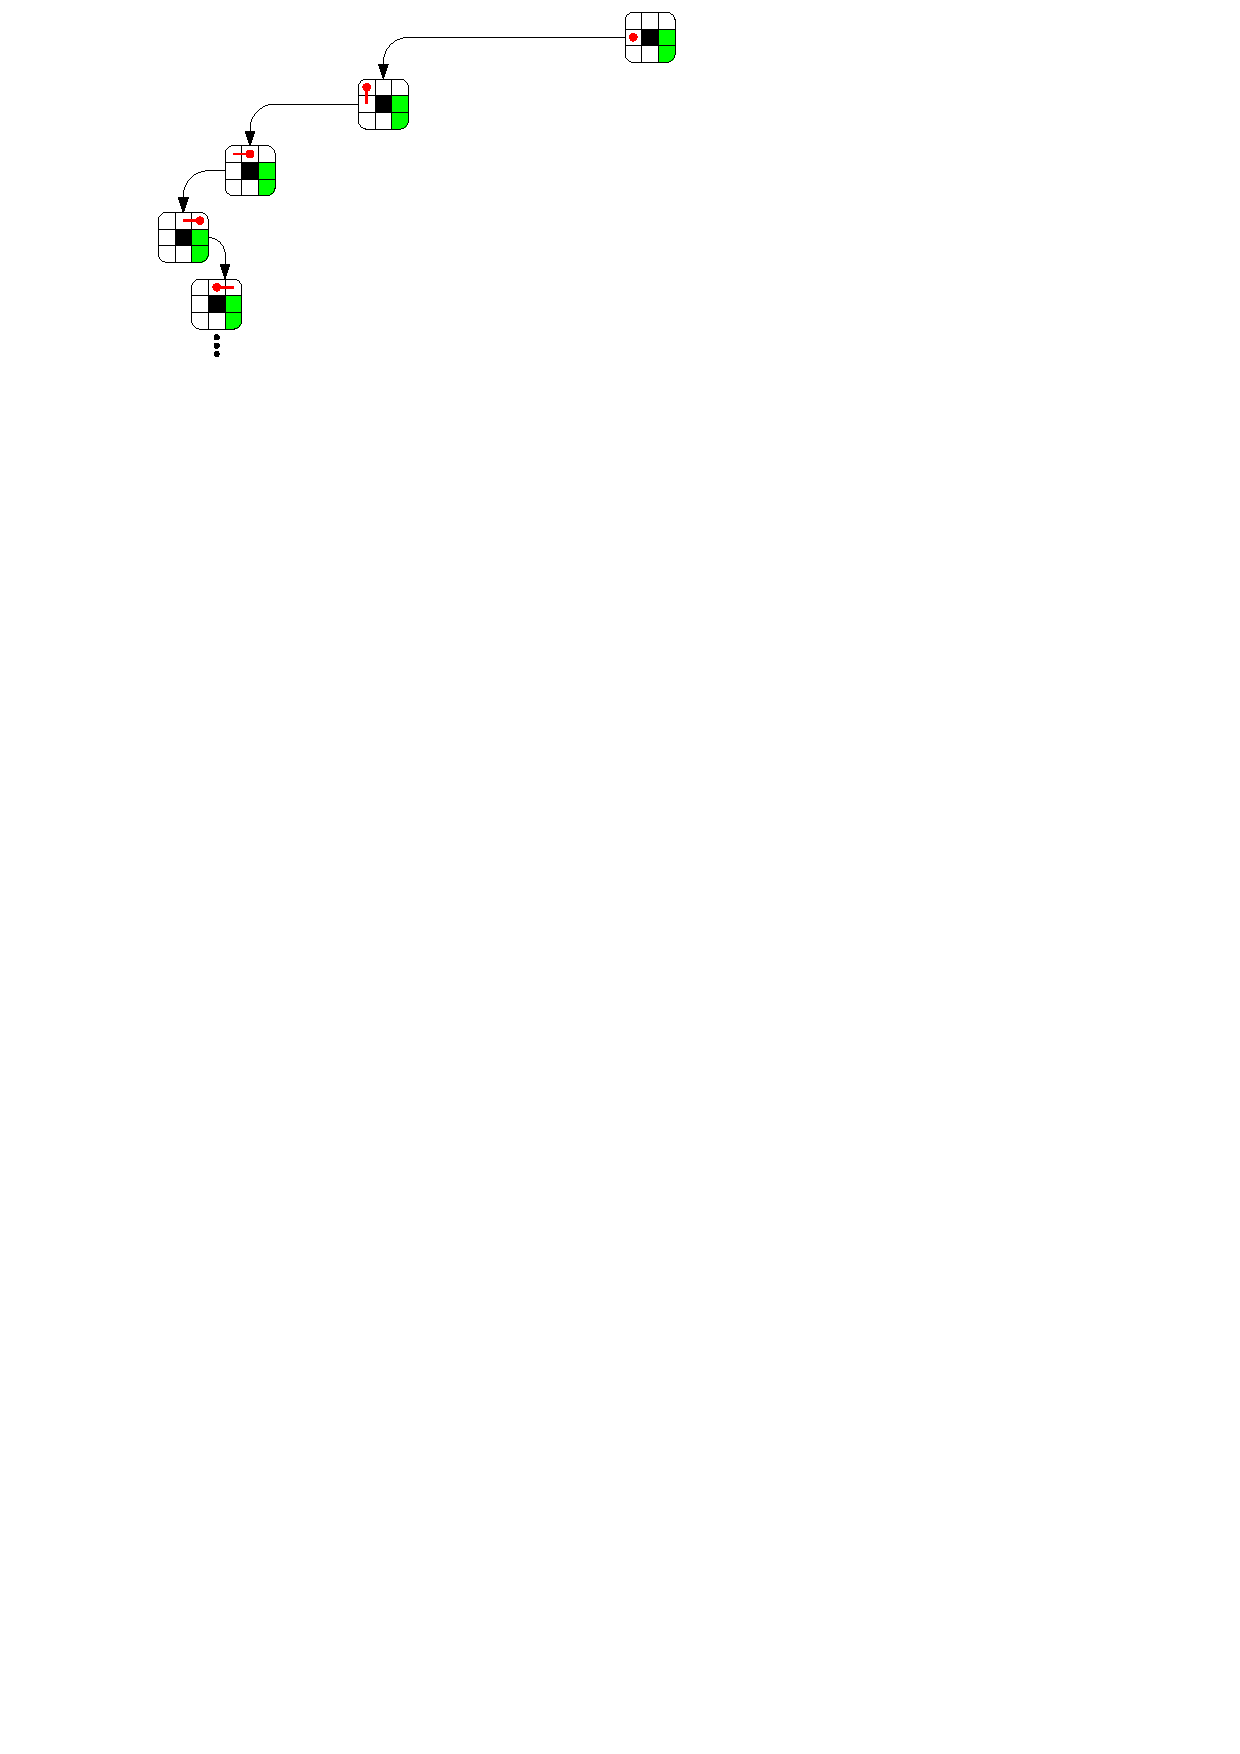
\includegraphics[width=\linewidth]{figs/dfs0.pdf}}%

  \only<9>{
    \begin{center}
      \Large Malá paměťová náročnost, ale bez garancí!
    \end{center}
  }
\end{frame}

\begin{frame}
  \frametitle{ID-DFS}

  \begin{center}
  	\LARGE Co když chceme jak garance, \\ tak malou paměťovou náročnost?
  \end{center}

  \vspace{2em}\hrule\vspace{2em}
  \hfill $\rightarrow$ Budeme prohledávat do \emph{omezené} hloubky
\end{frame}

\begin{frame}[t]
  \frametitle{ID-DFS}

  \vspace{3em}

  \only<1>{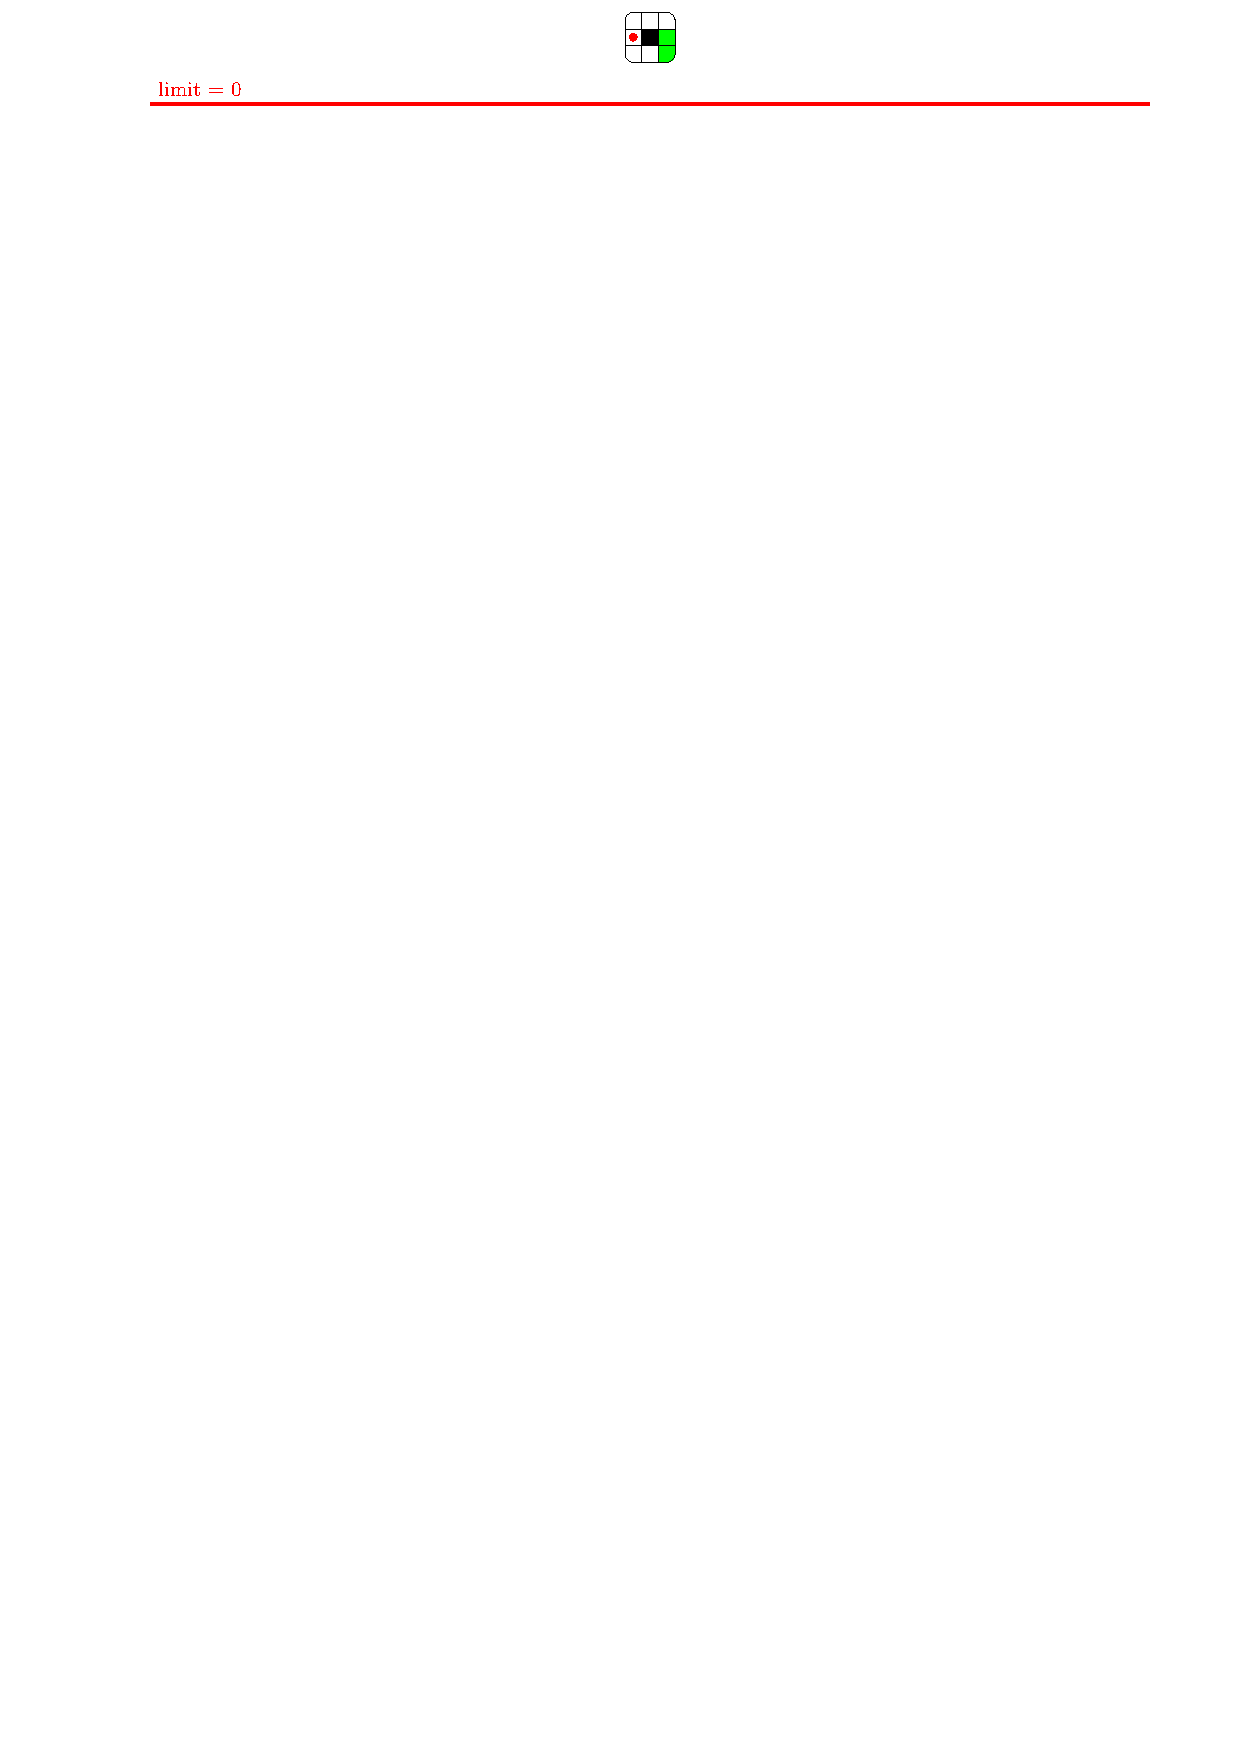
\includegraphics[width=\linewidth]{figs/iddfs26.pdf}}%
  \only<2>{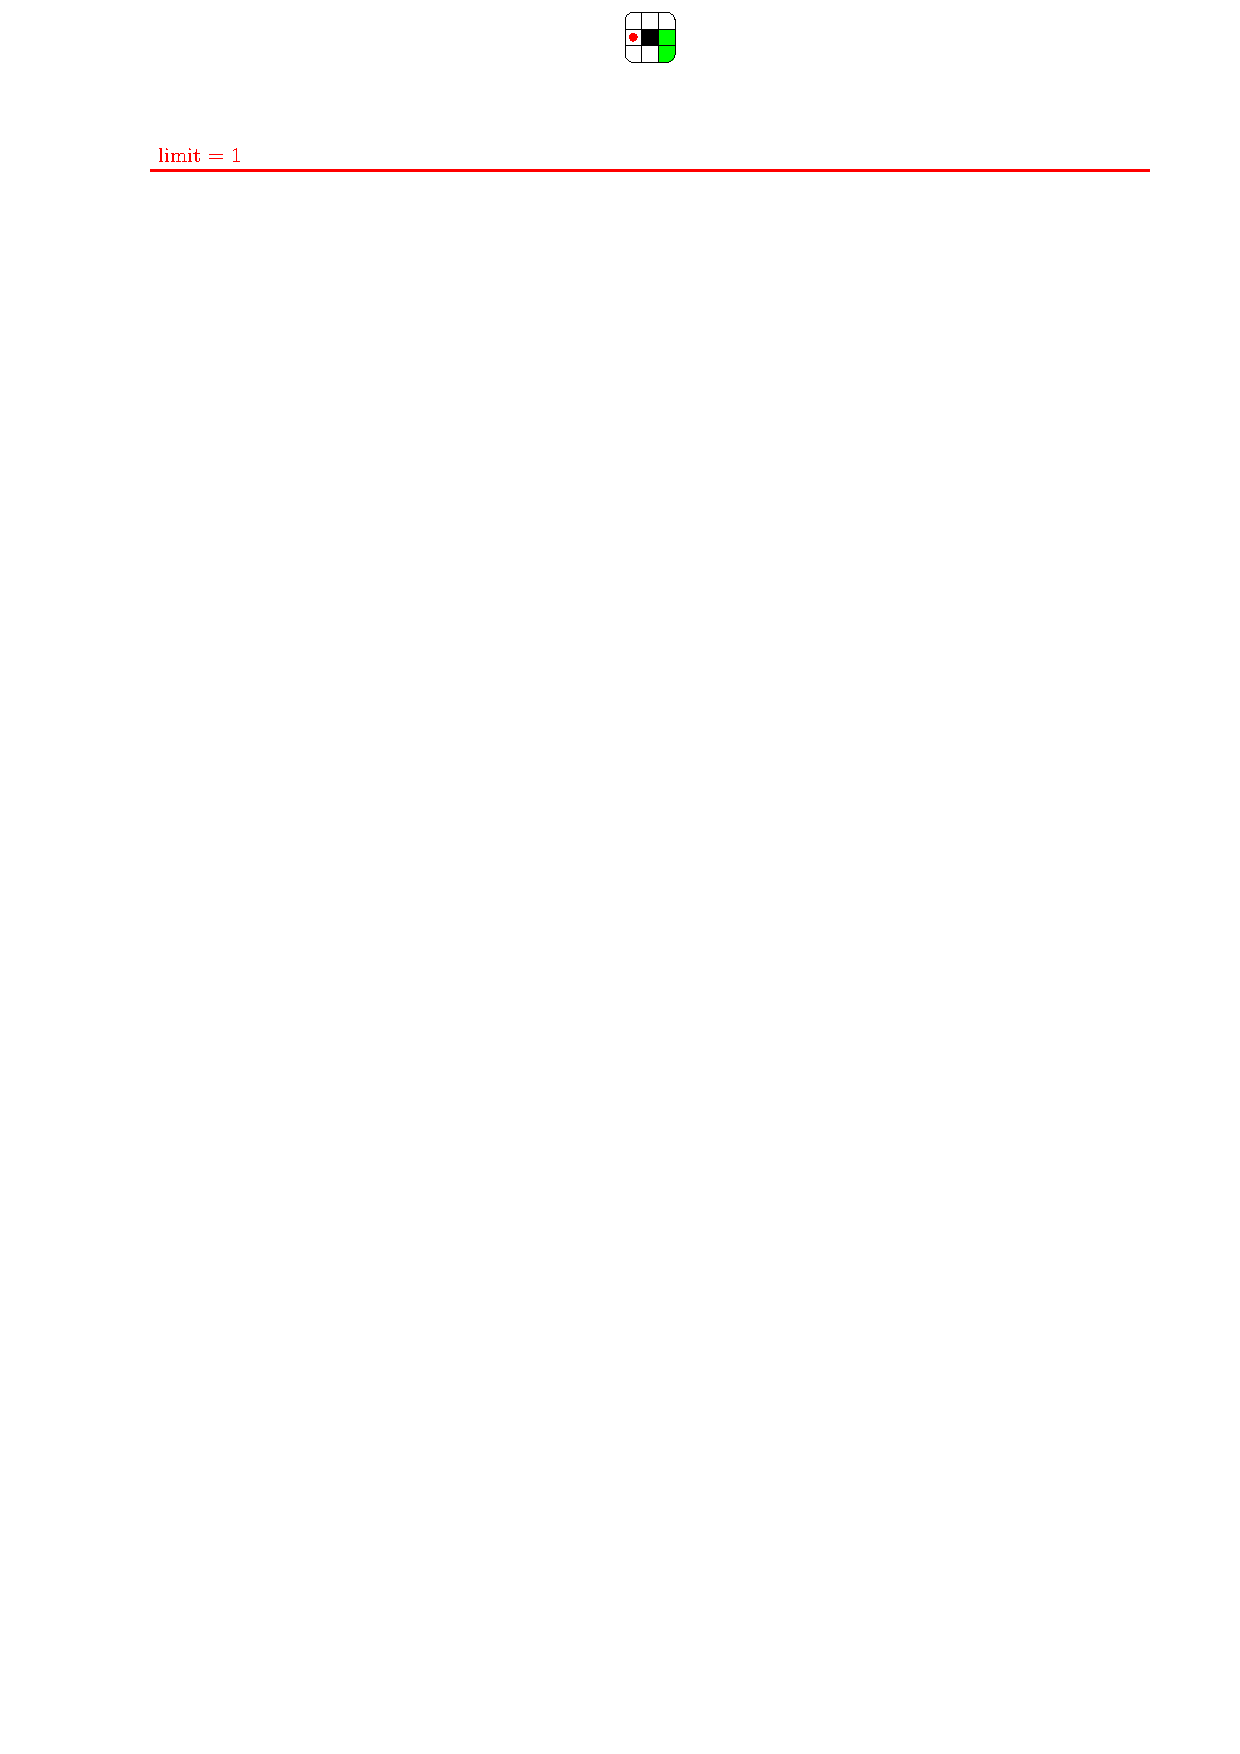
\includegraphics[width=\linewidth]{figs/iddfs25.pdf}}%
  \only<3>{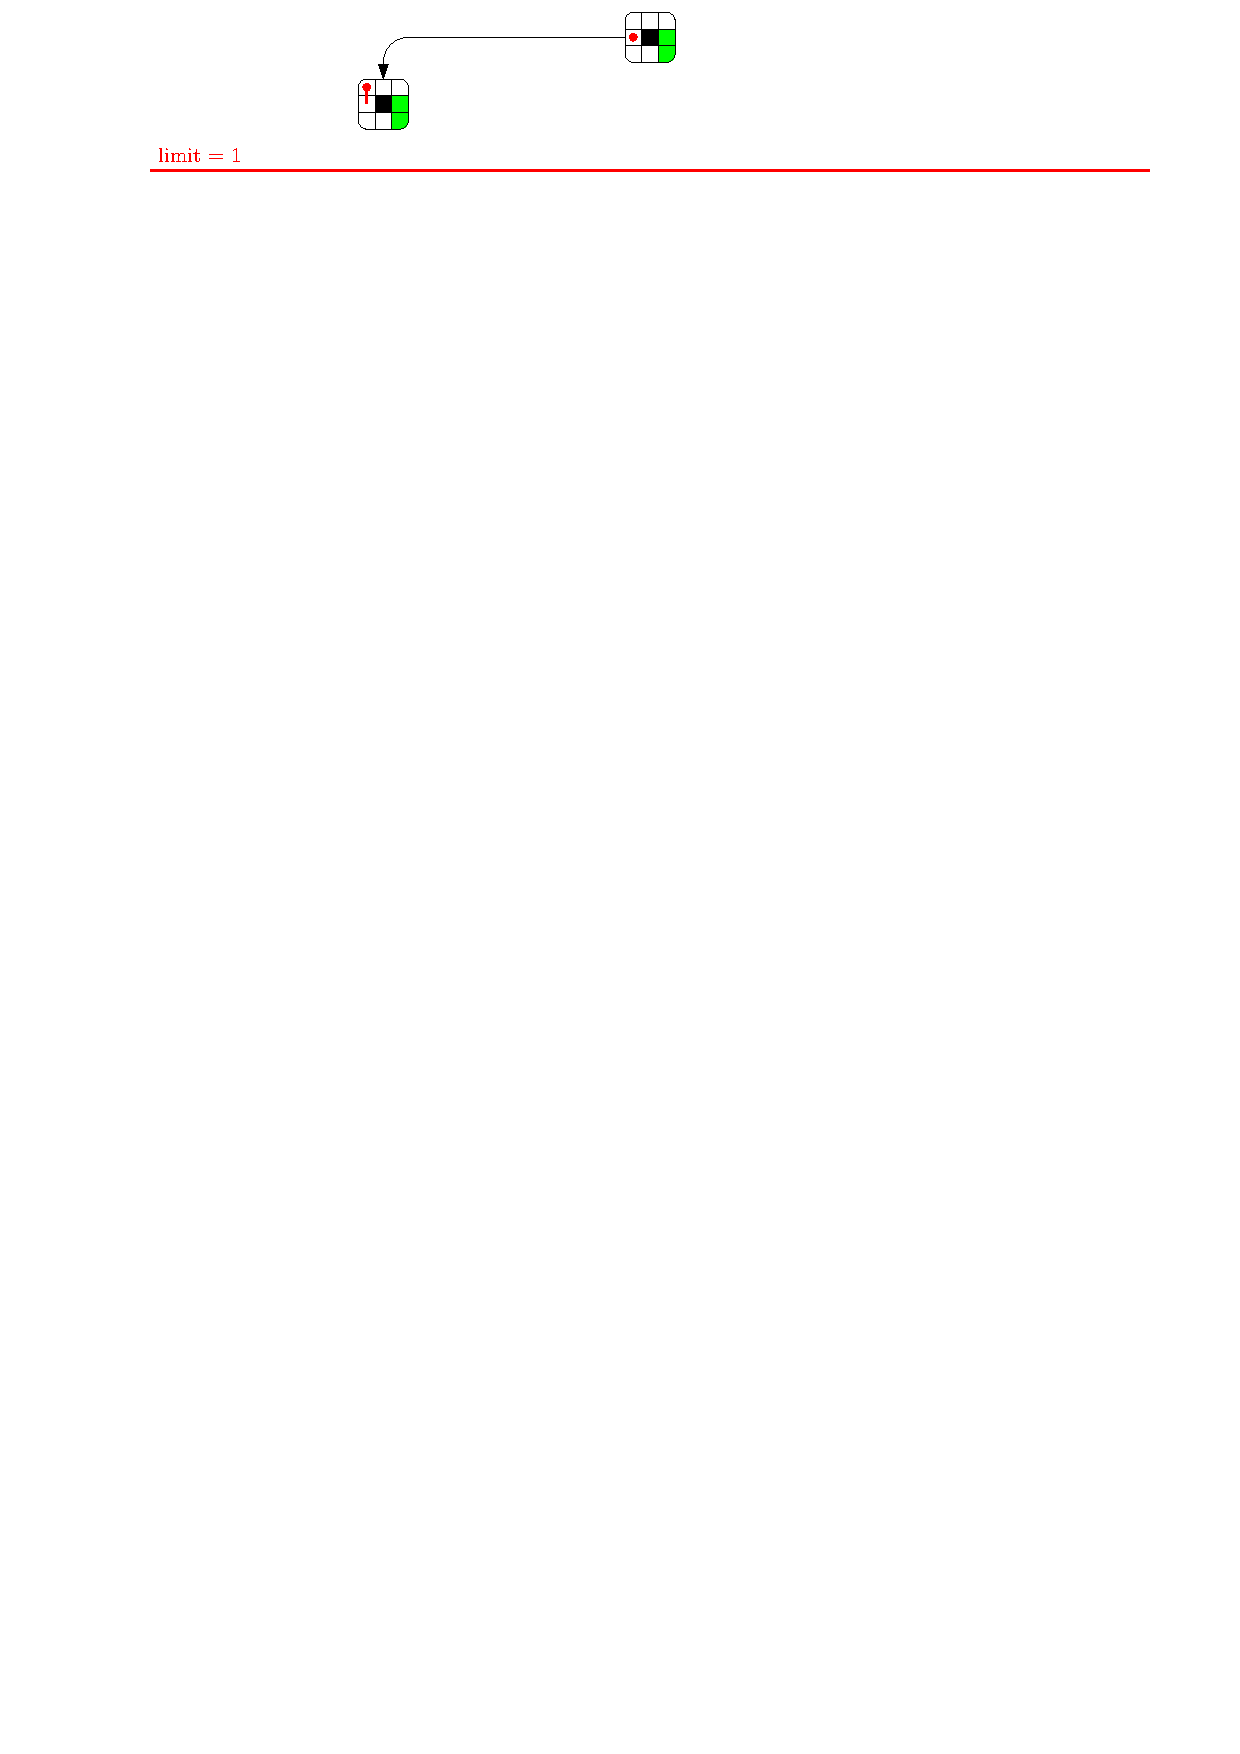
\includegraphics[width=\linewidth]{figs/iddfs24.pdf}}%
  \only<4>{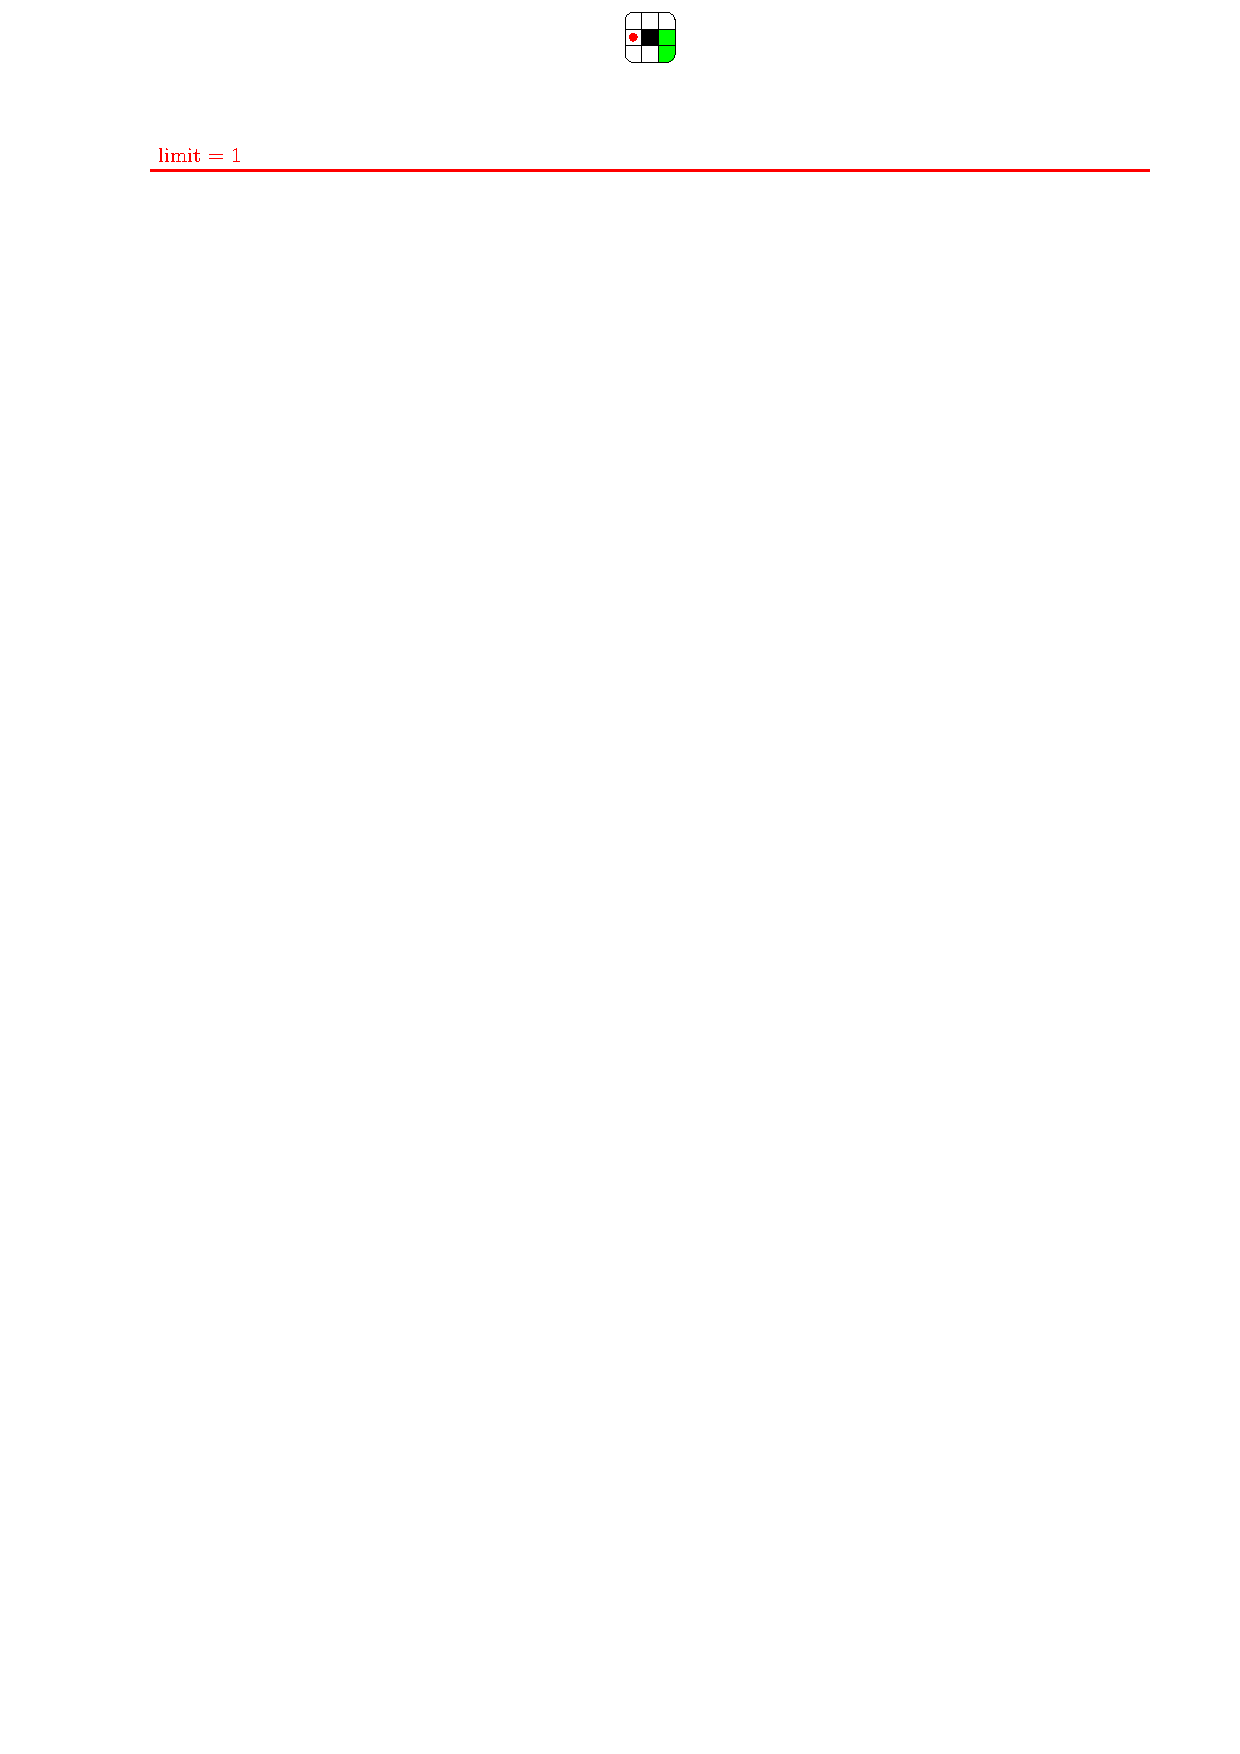
\includegraphics[width=\linewidth]{figs/iddfs25.pdf}}%
  \only<5>{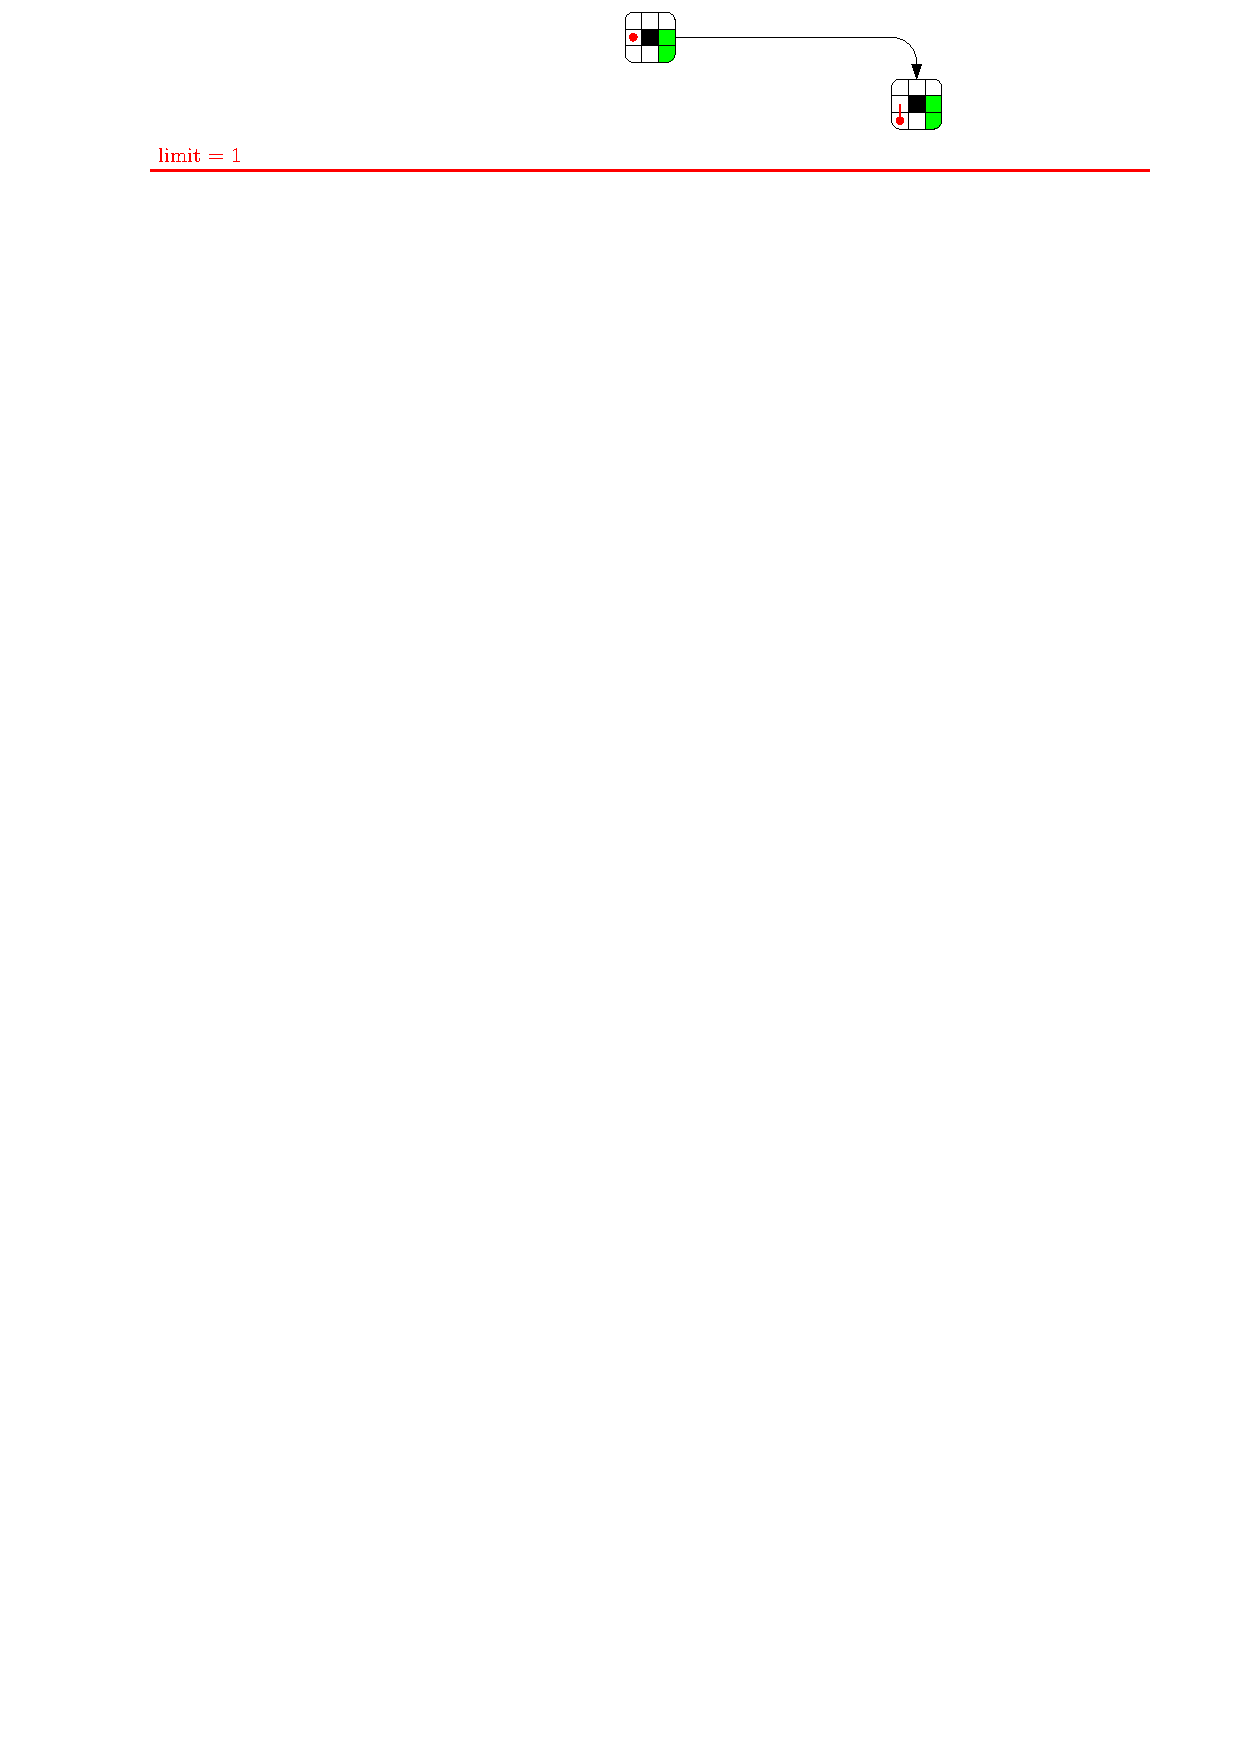
\includegraphics[width=\linewidth]{figs/iddfs23.pdf}}%
  \only<6>{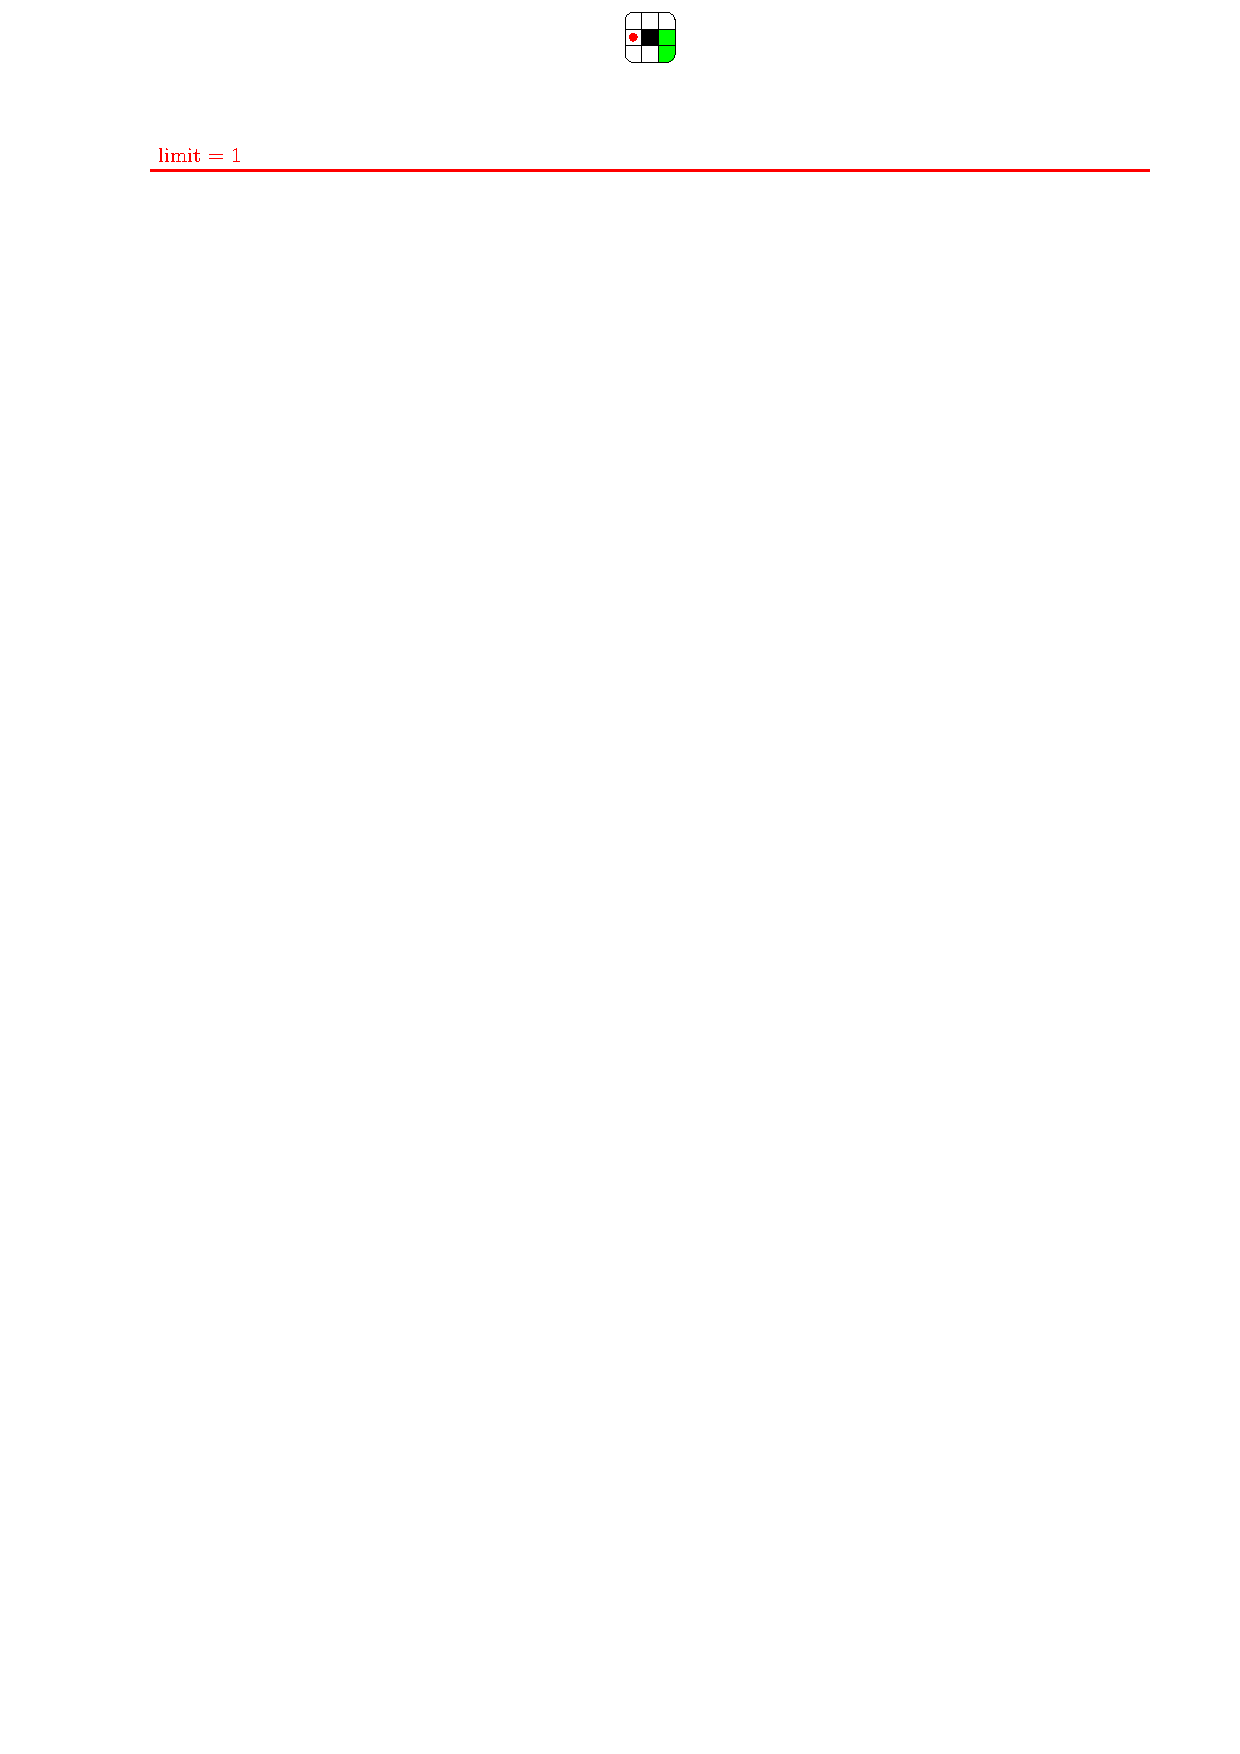
\includegraphics[width=\linewidth]{figs/iddfs25.pdf}}%
  \only<7>{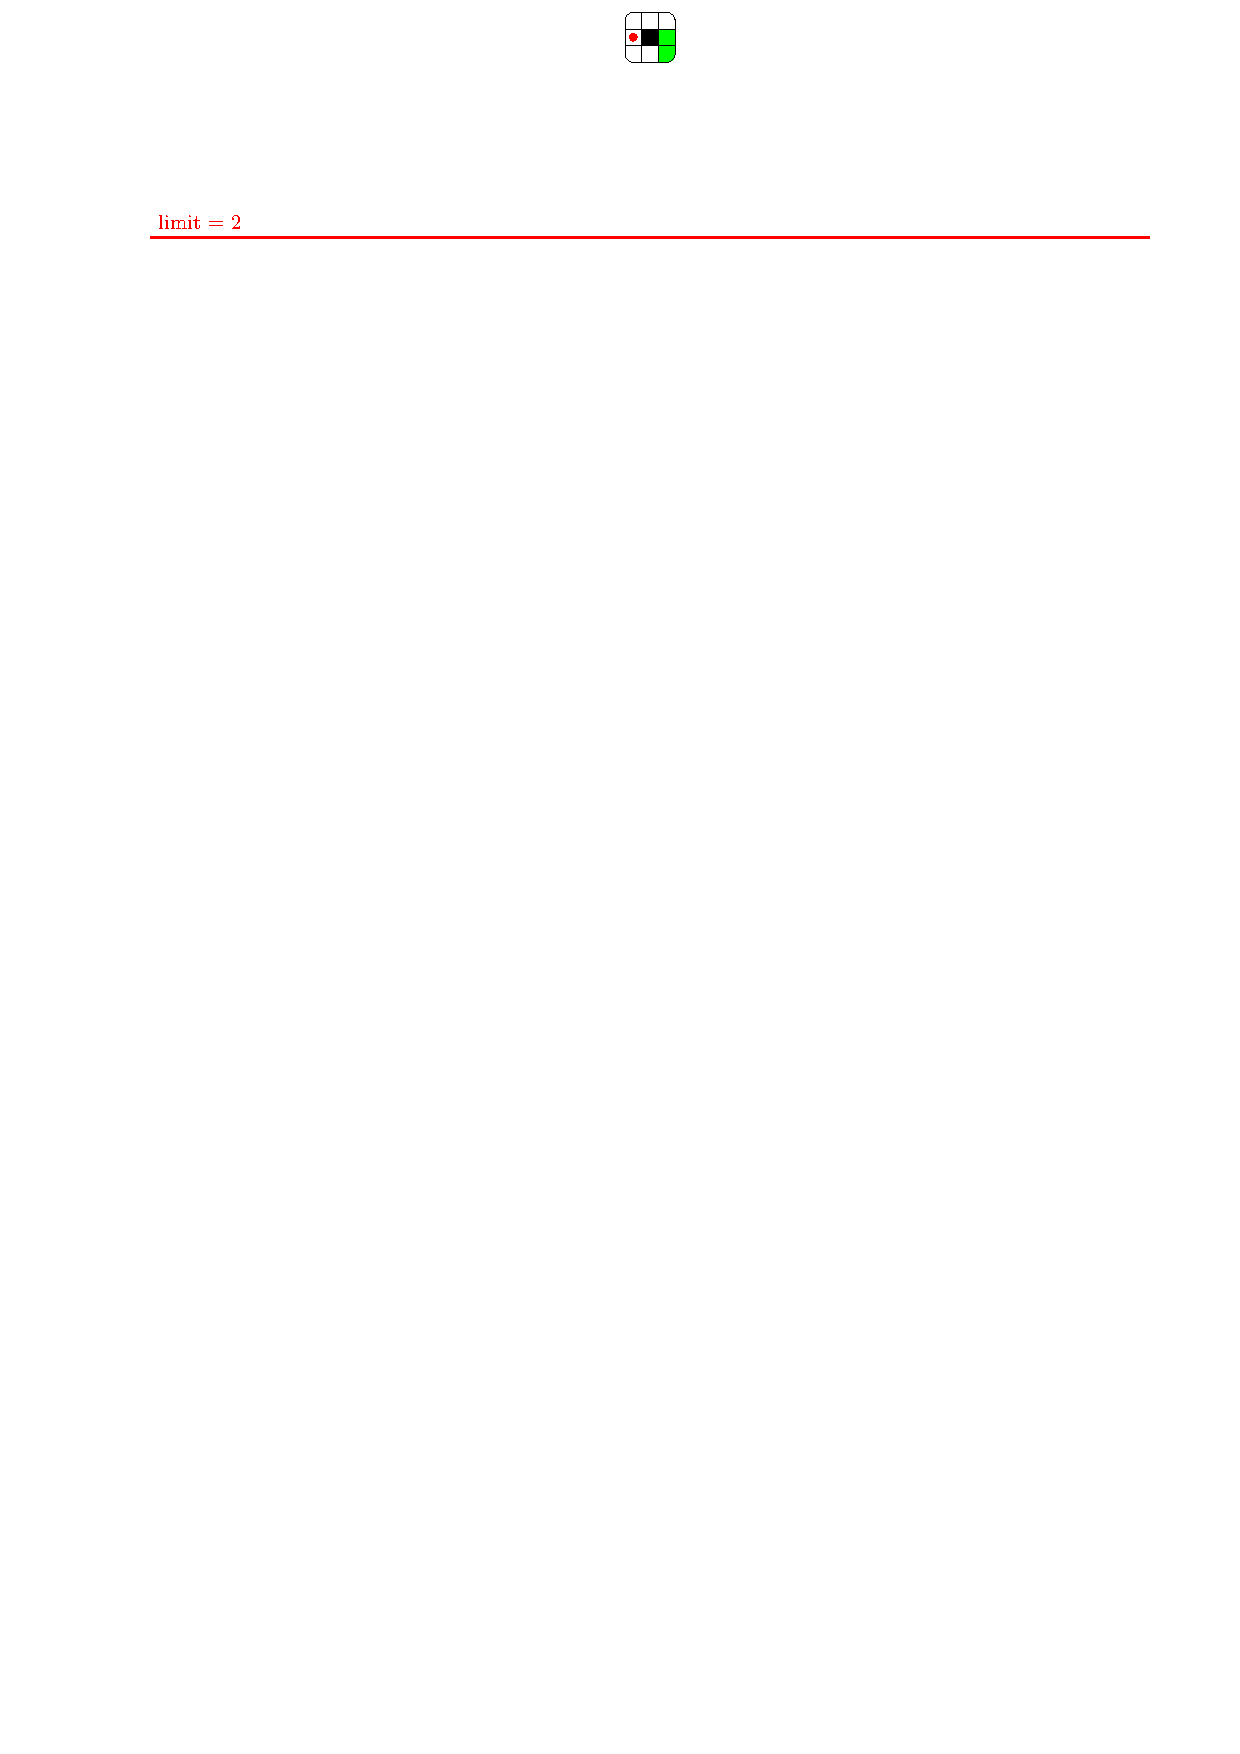
\includegraphics[width=\linewidth]{figs/iddfs22.pdf}}%
  \only<8>{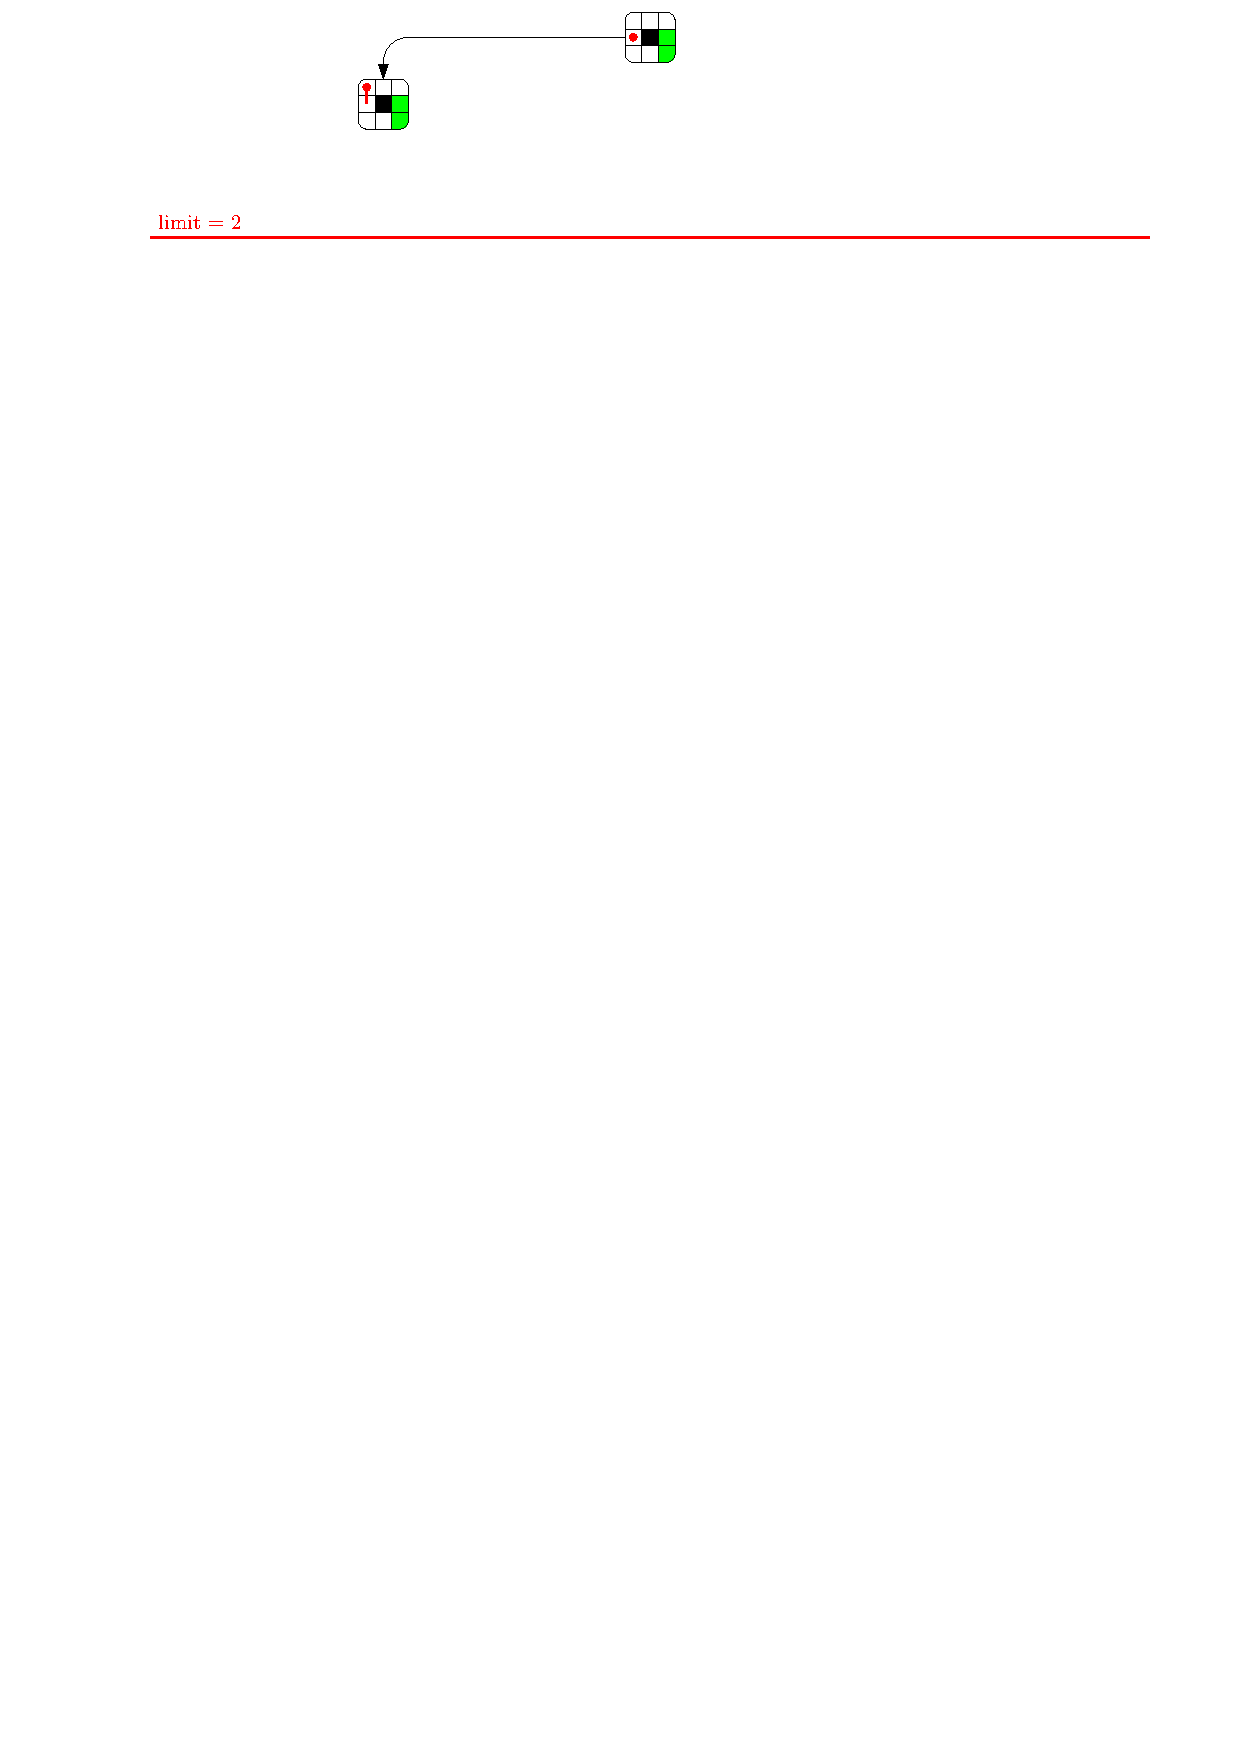
\includegraphics[width=\linewidth]{figs/iddfs21.pdf}}%
  \only<9>{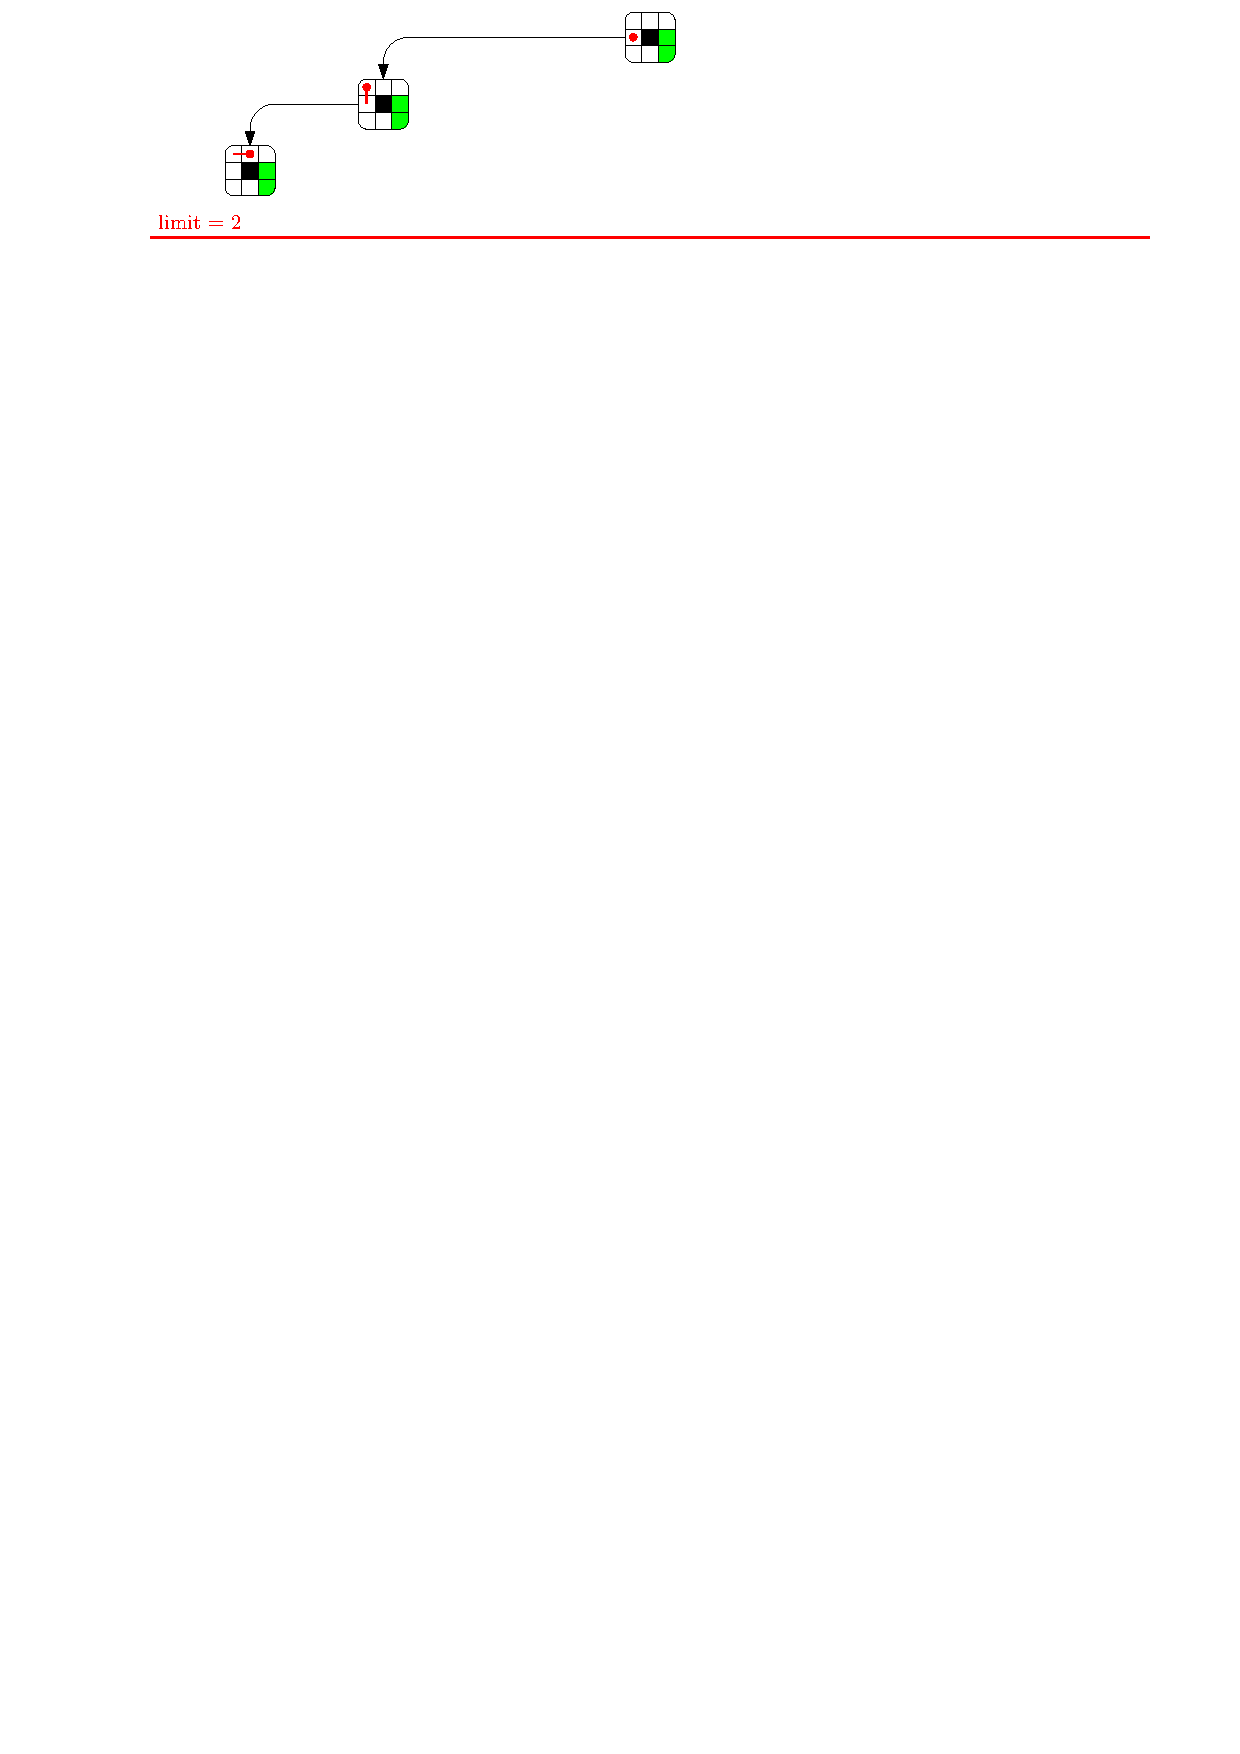
\includegraphics[width=\linewidth]{figs/iddfs20.pdf}}%
  \only<10>{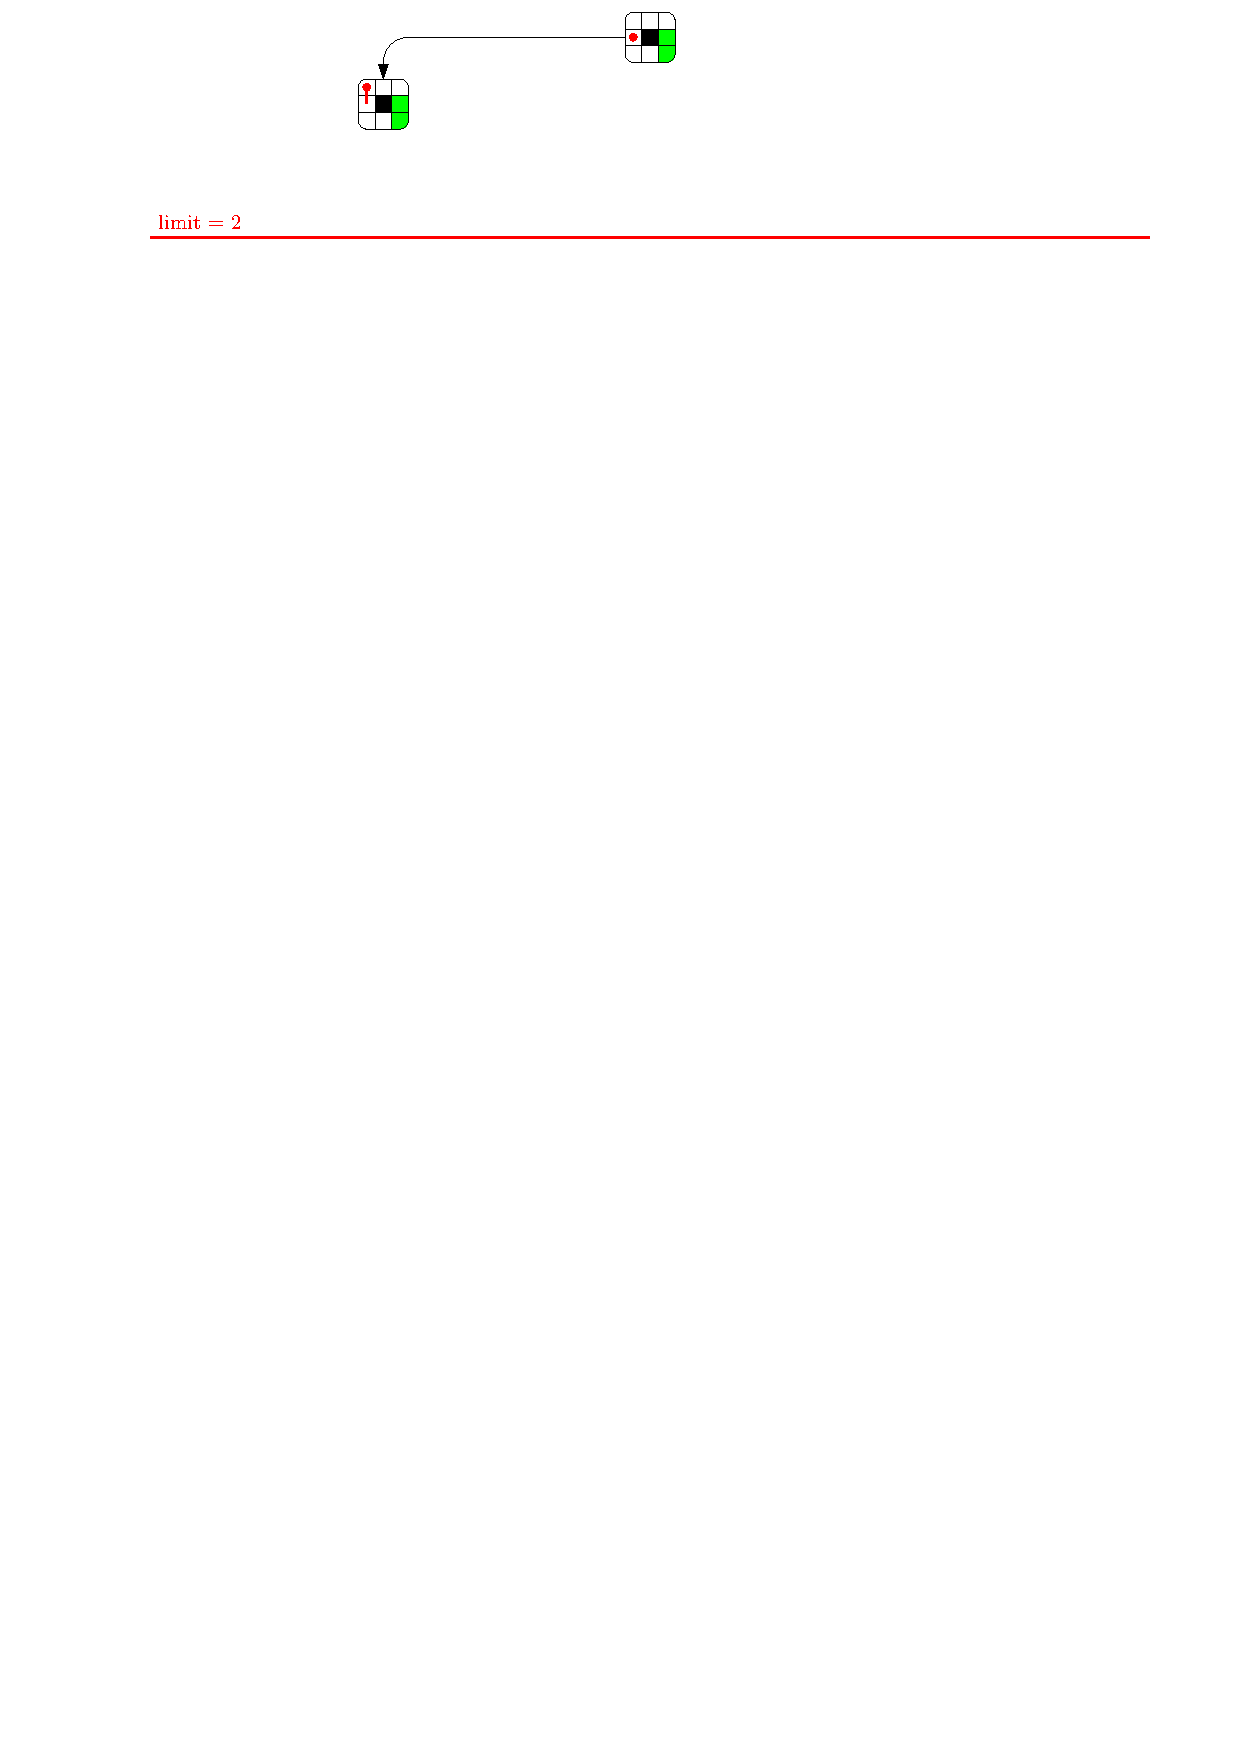
\includegraphics[width=\linewidth]{figs/iddfs21.pdf}}%
  \only<11>{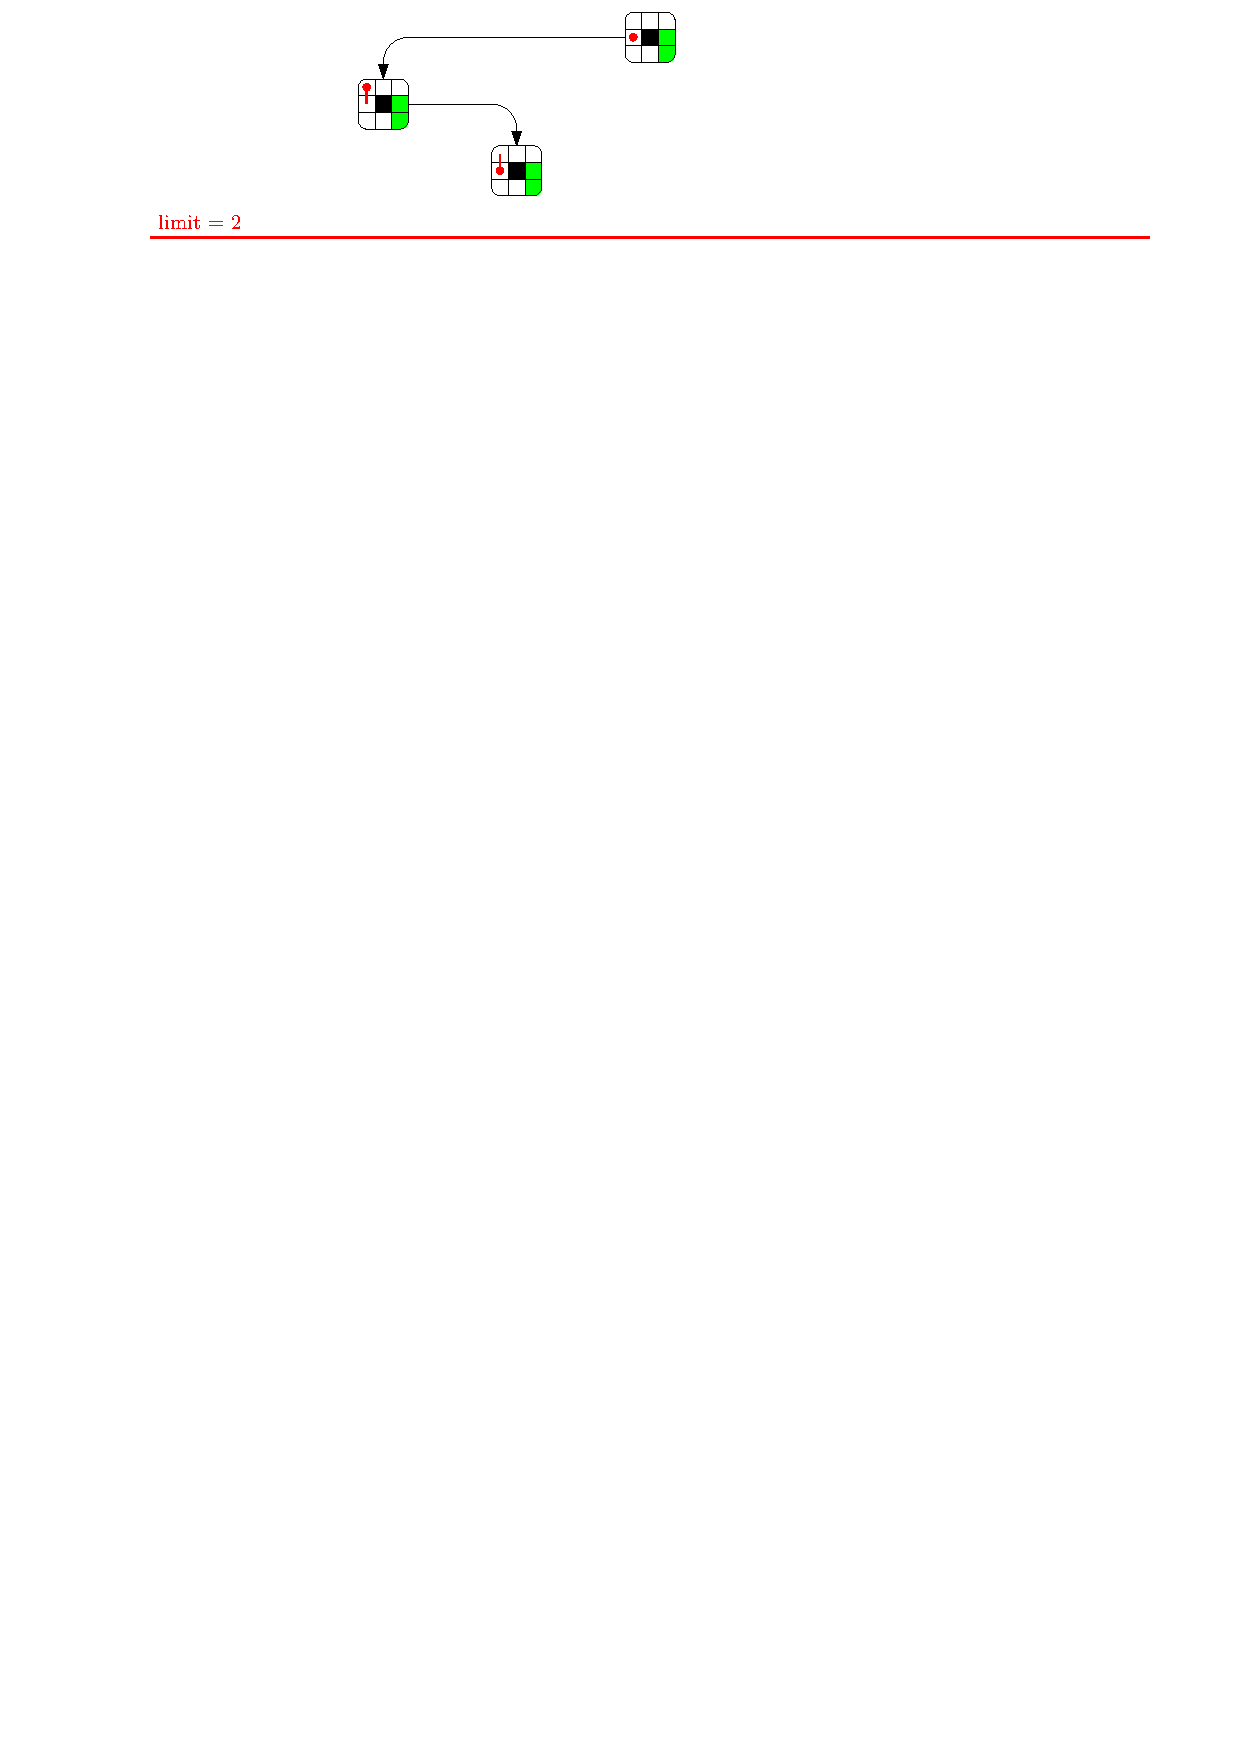
\includegraphics[width=\linewidth]{figs/iddfs19.pdf}}%
  \only<12>{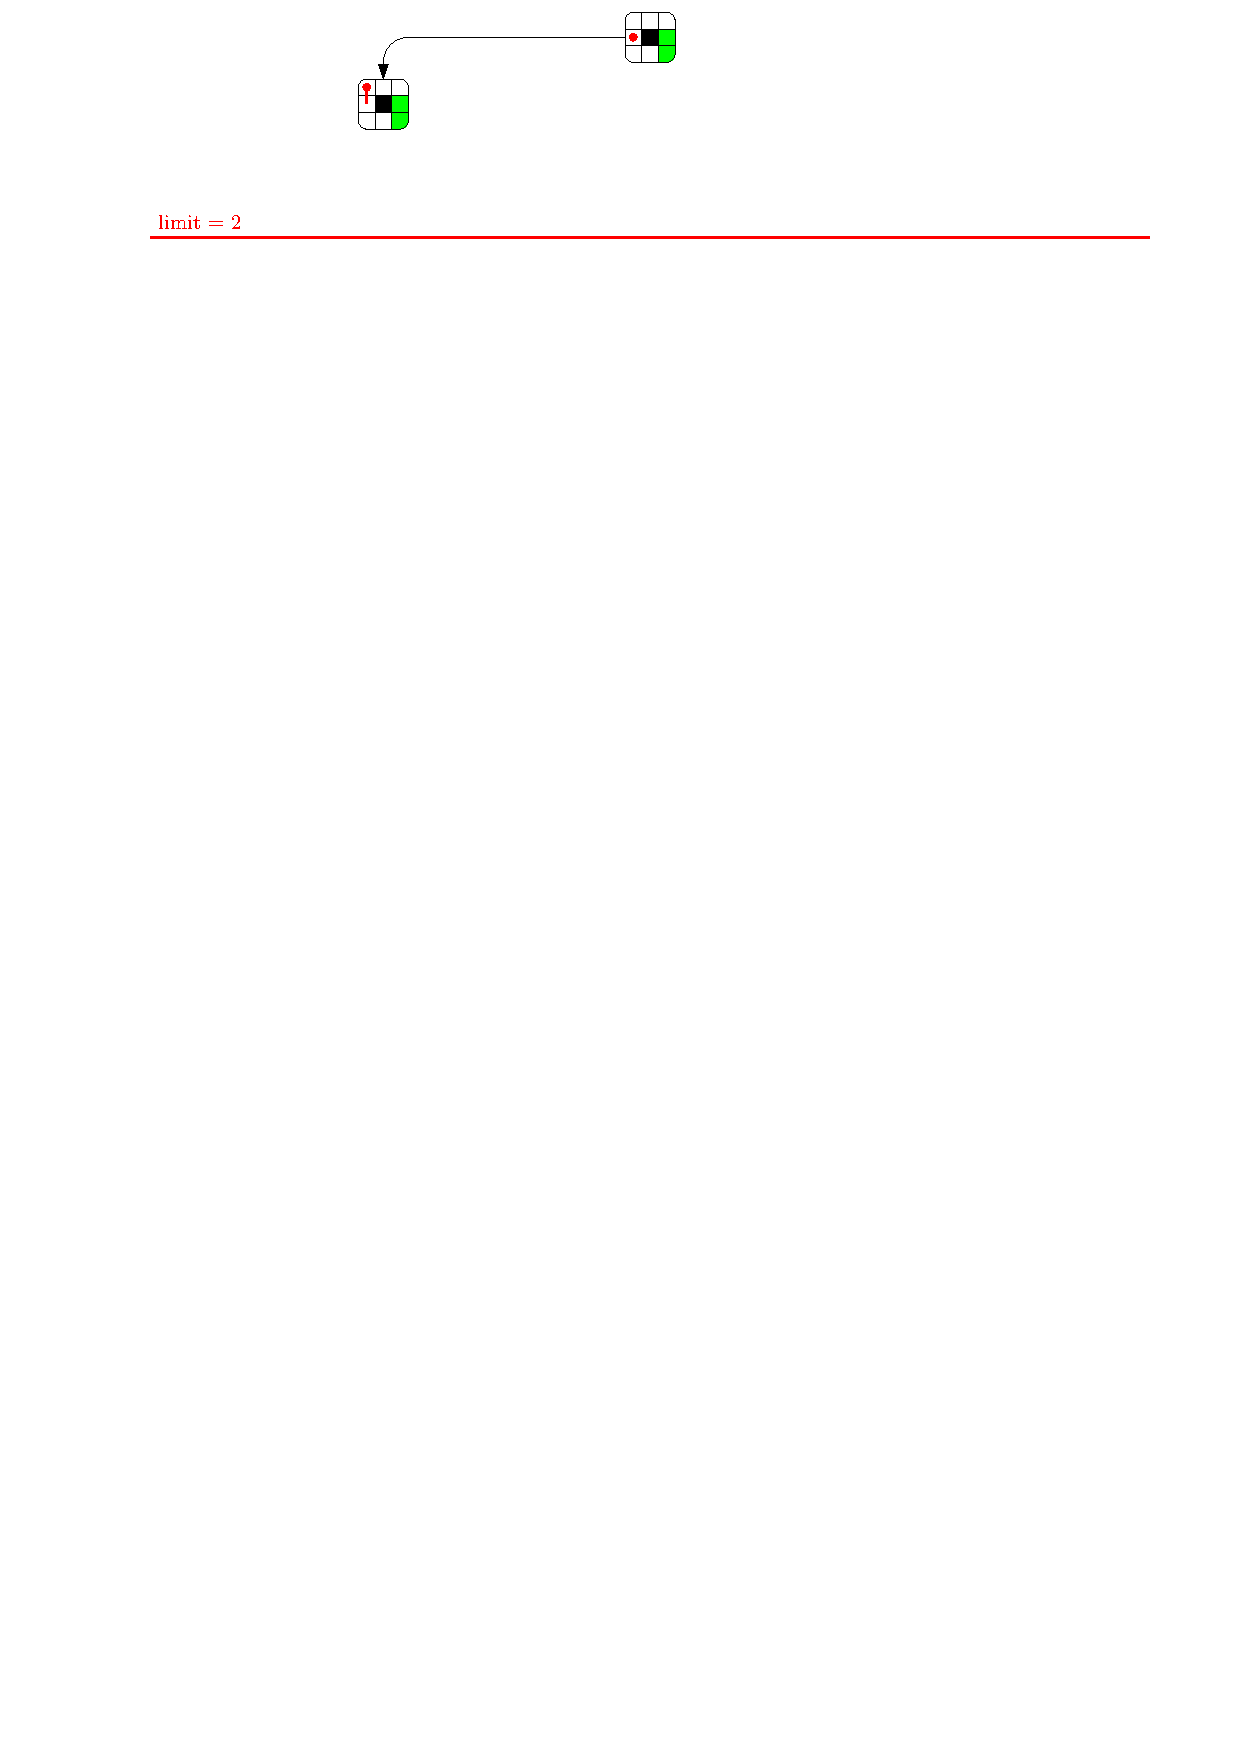
\includegraphics[width=\linewidth]{figs/iddfs21.pdf}}%
  \only<13>{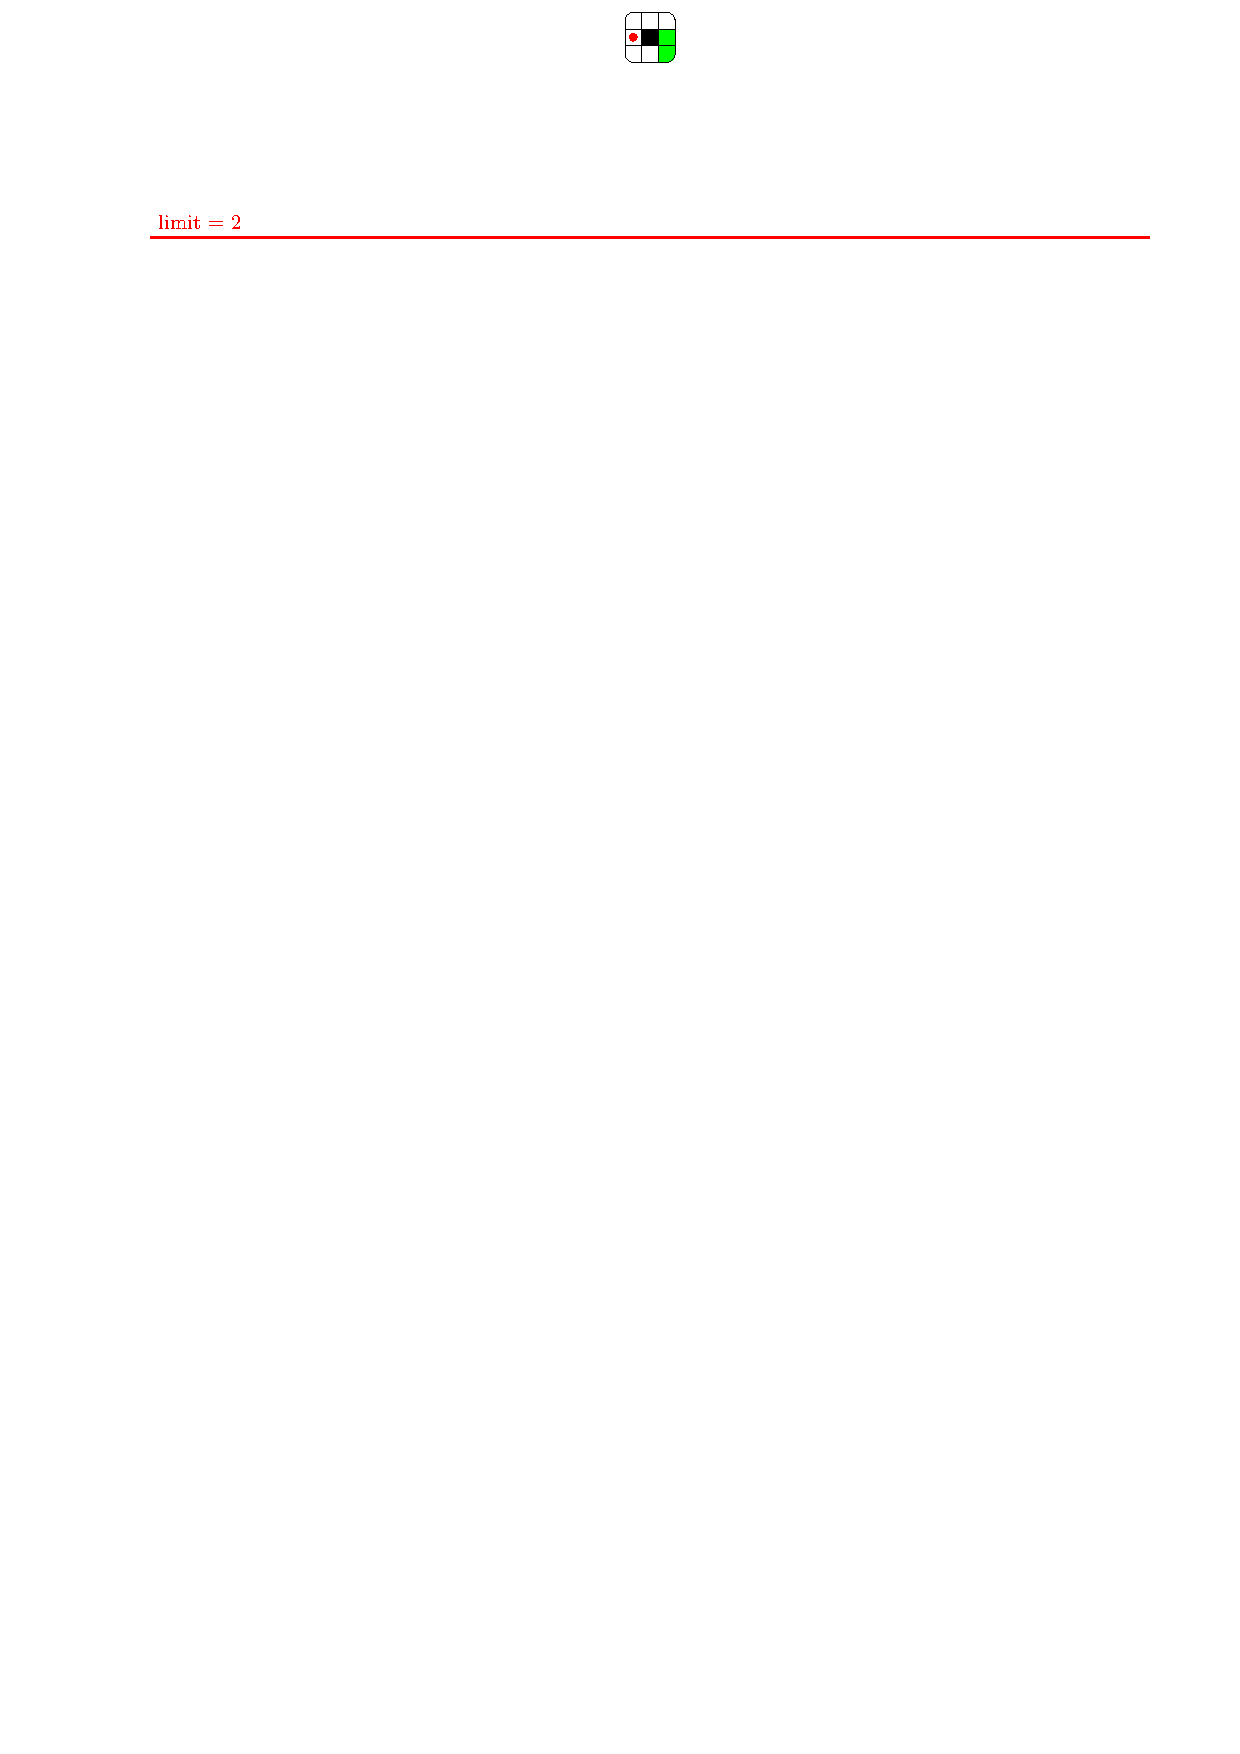
\includegraphics[width=\linewidth]{figs/iddfs22.pdf}}%
  \only<14>{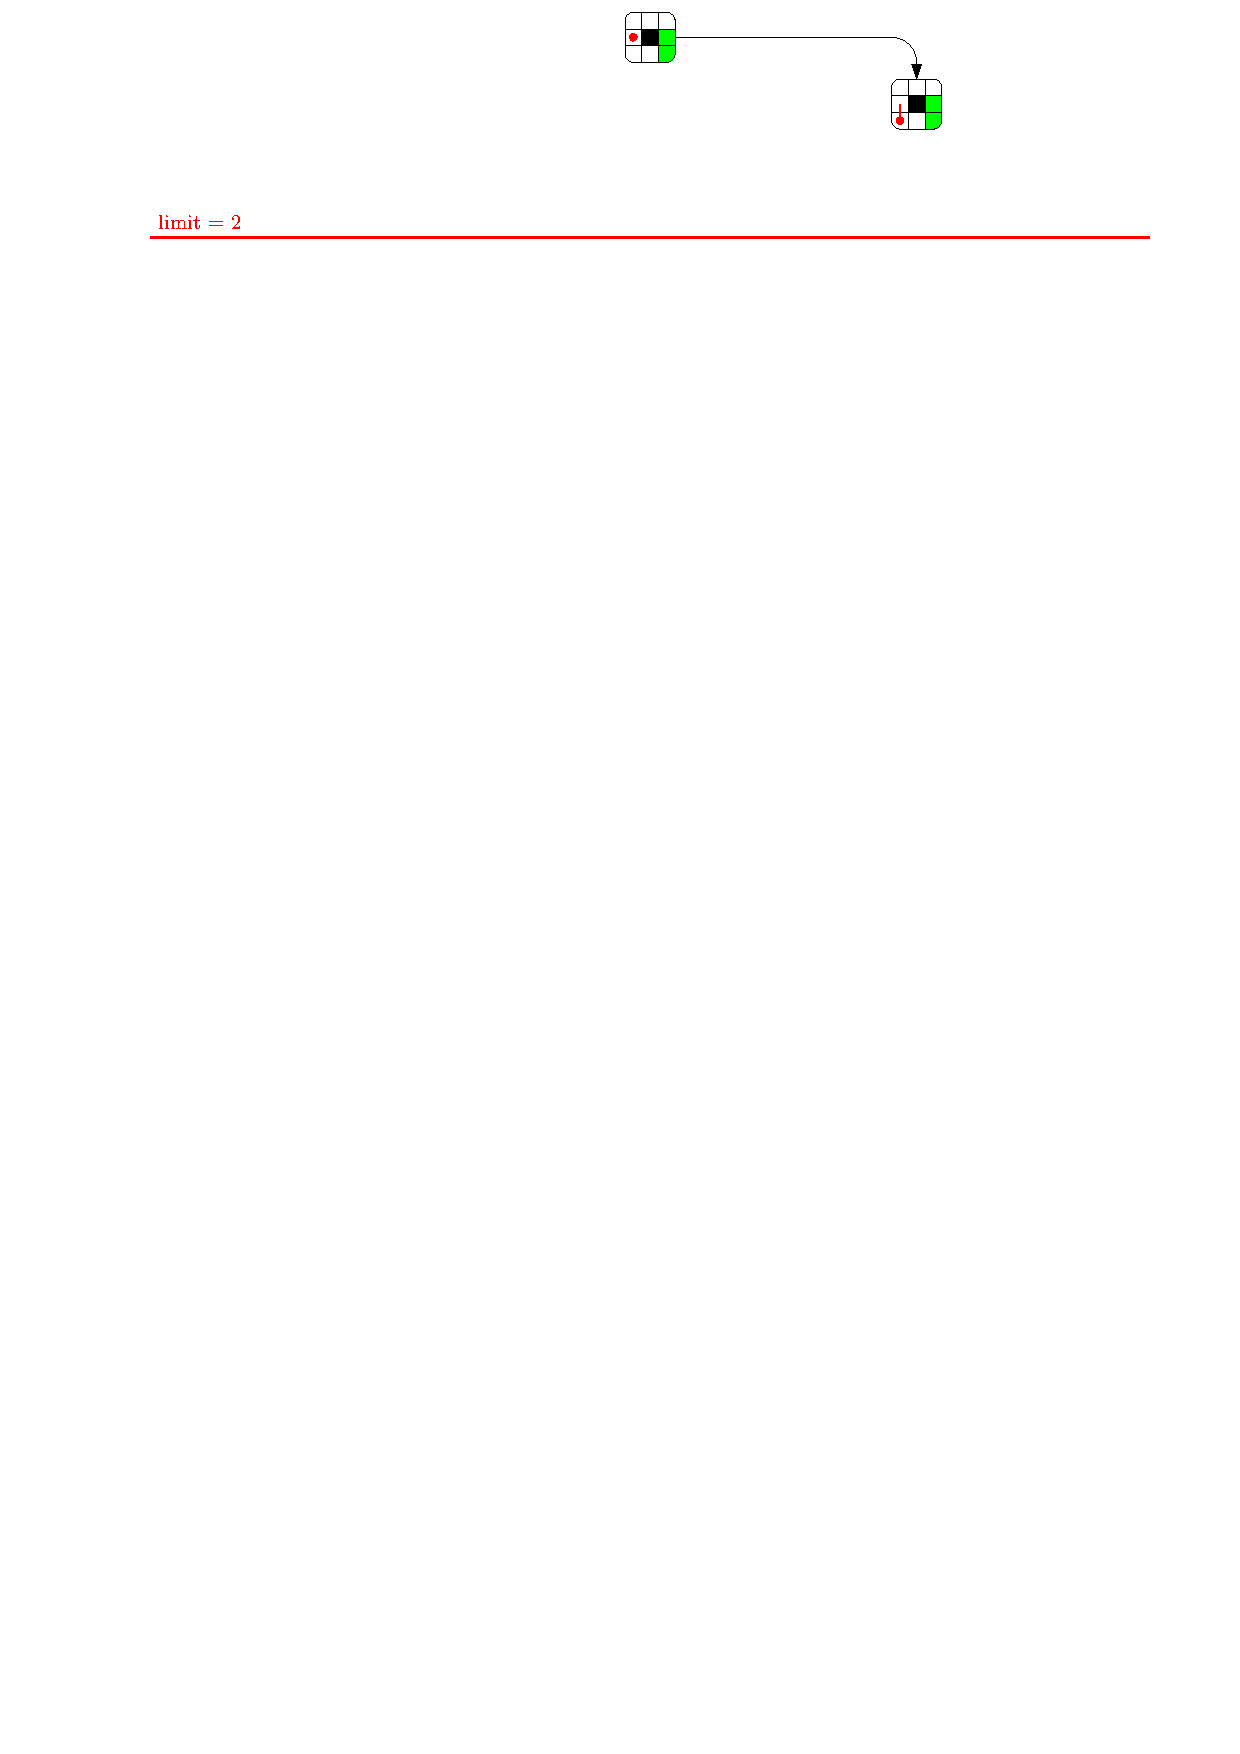
\includegraphics[width=\linewidth]{figs/iddfs18.pdf}}%
  \only<15>{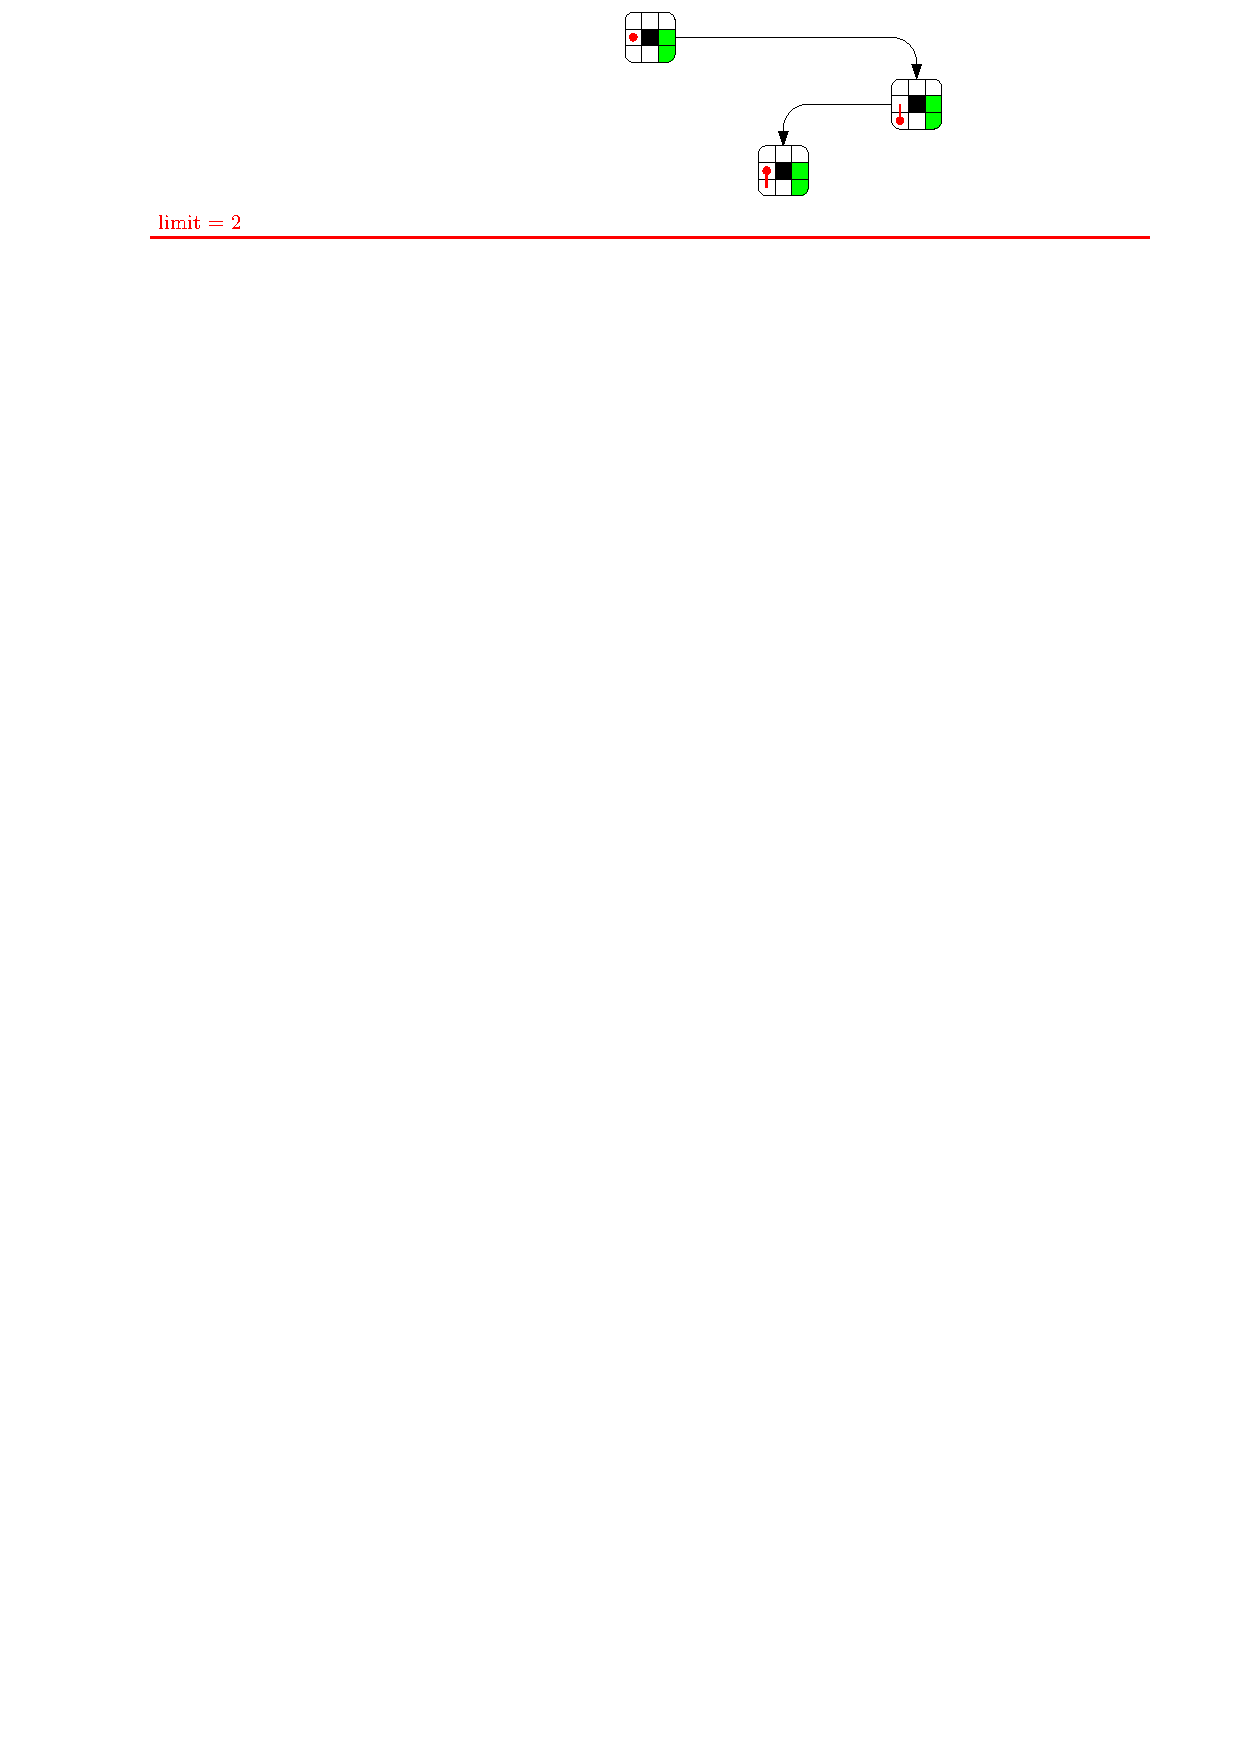
\includegraphics[width=\linewidth]{figs/iddfs17.pdf}}%
  \only<16>{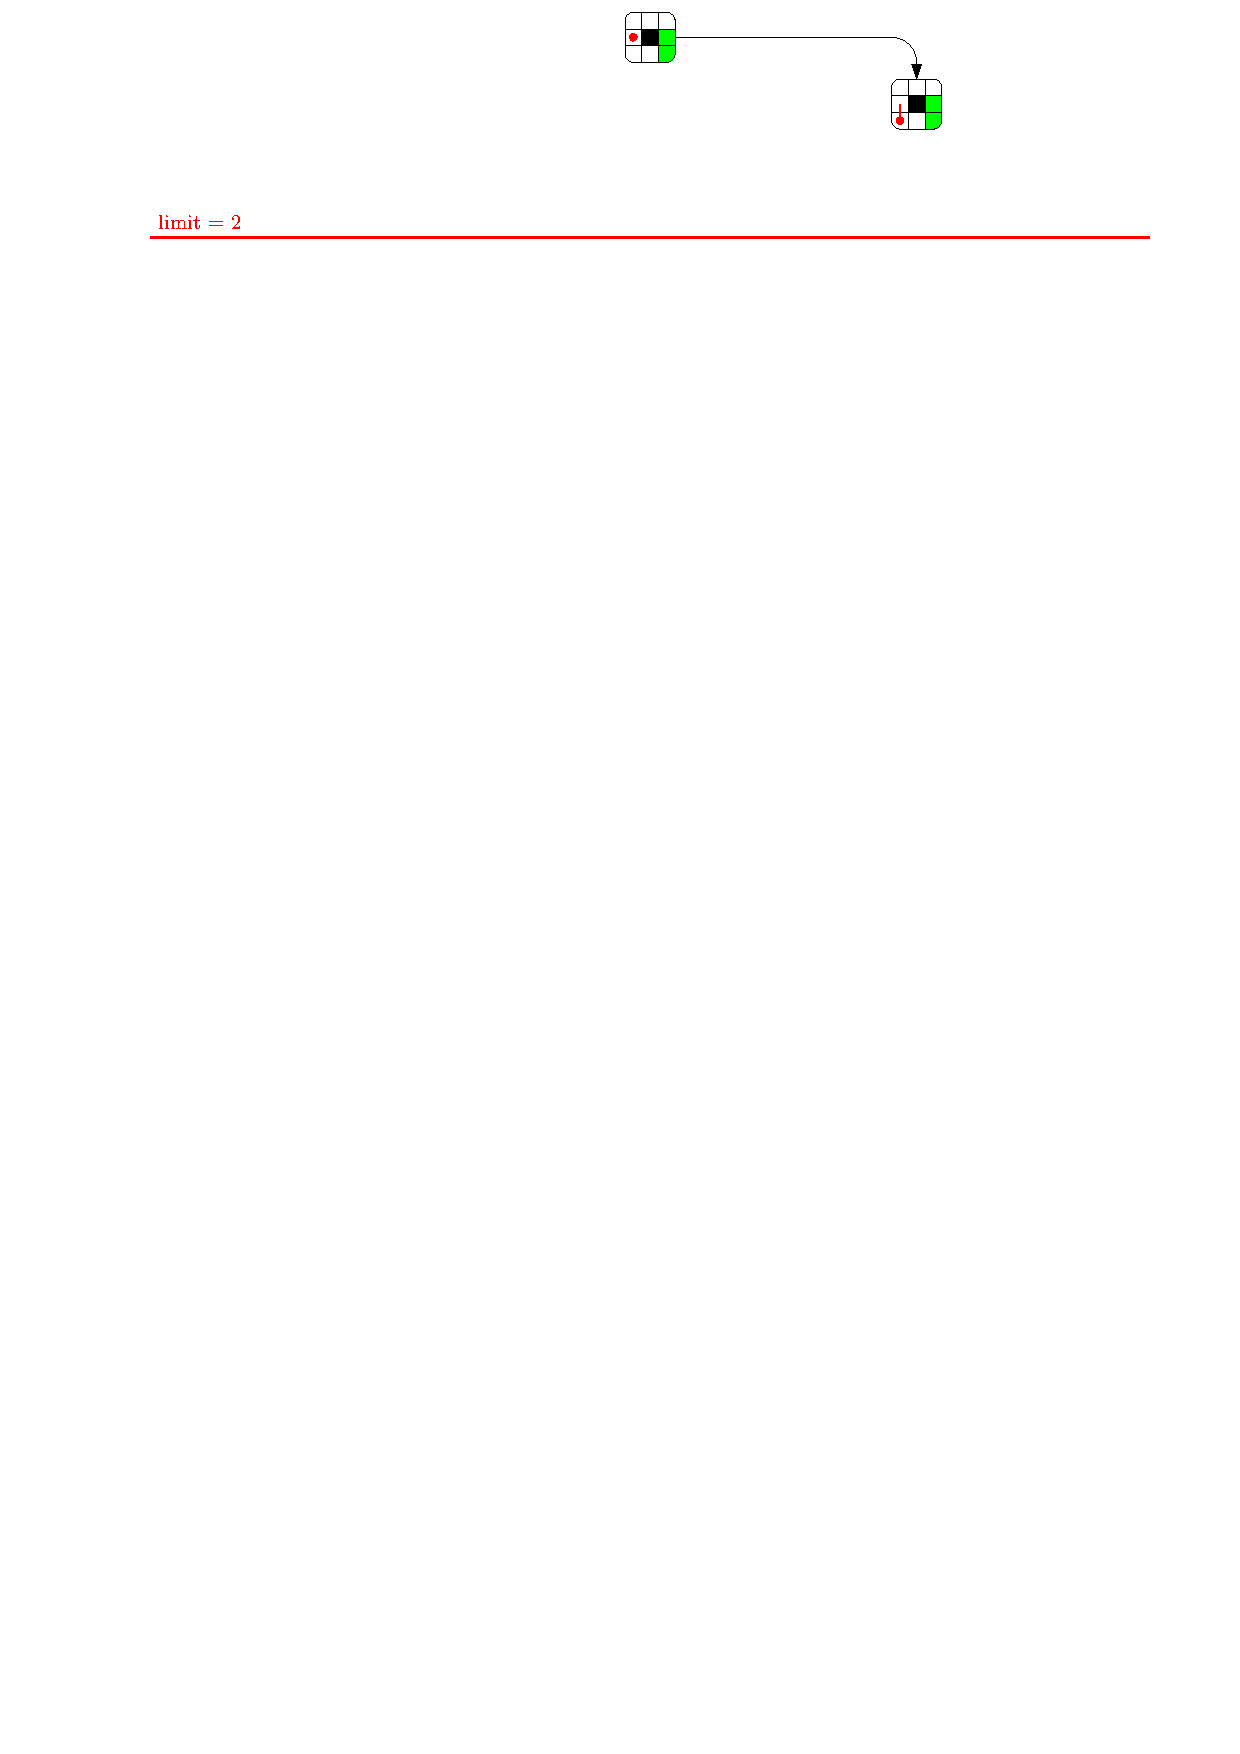
\includegraphics[width=\linewidth]{figs/iddfs18.pdf}}%
  \only<17>{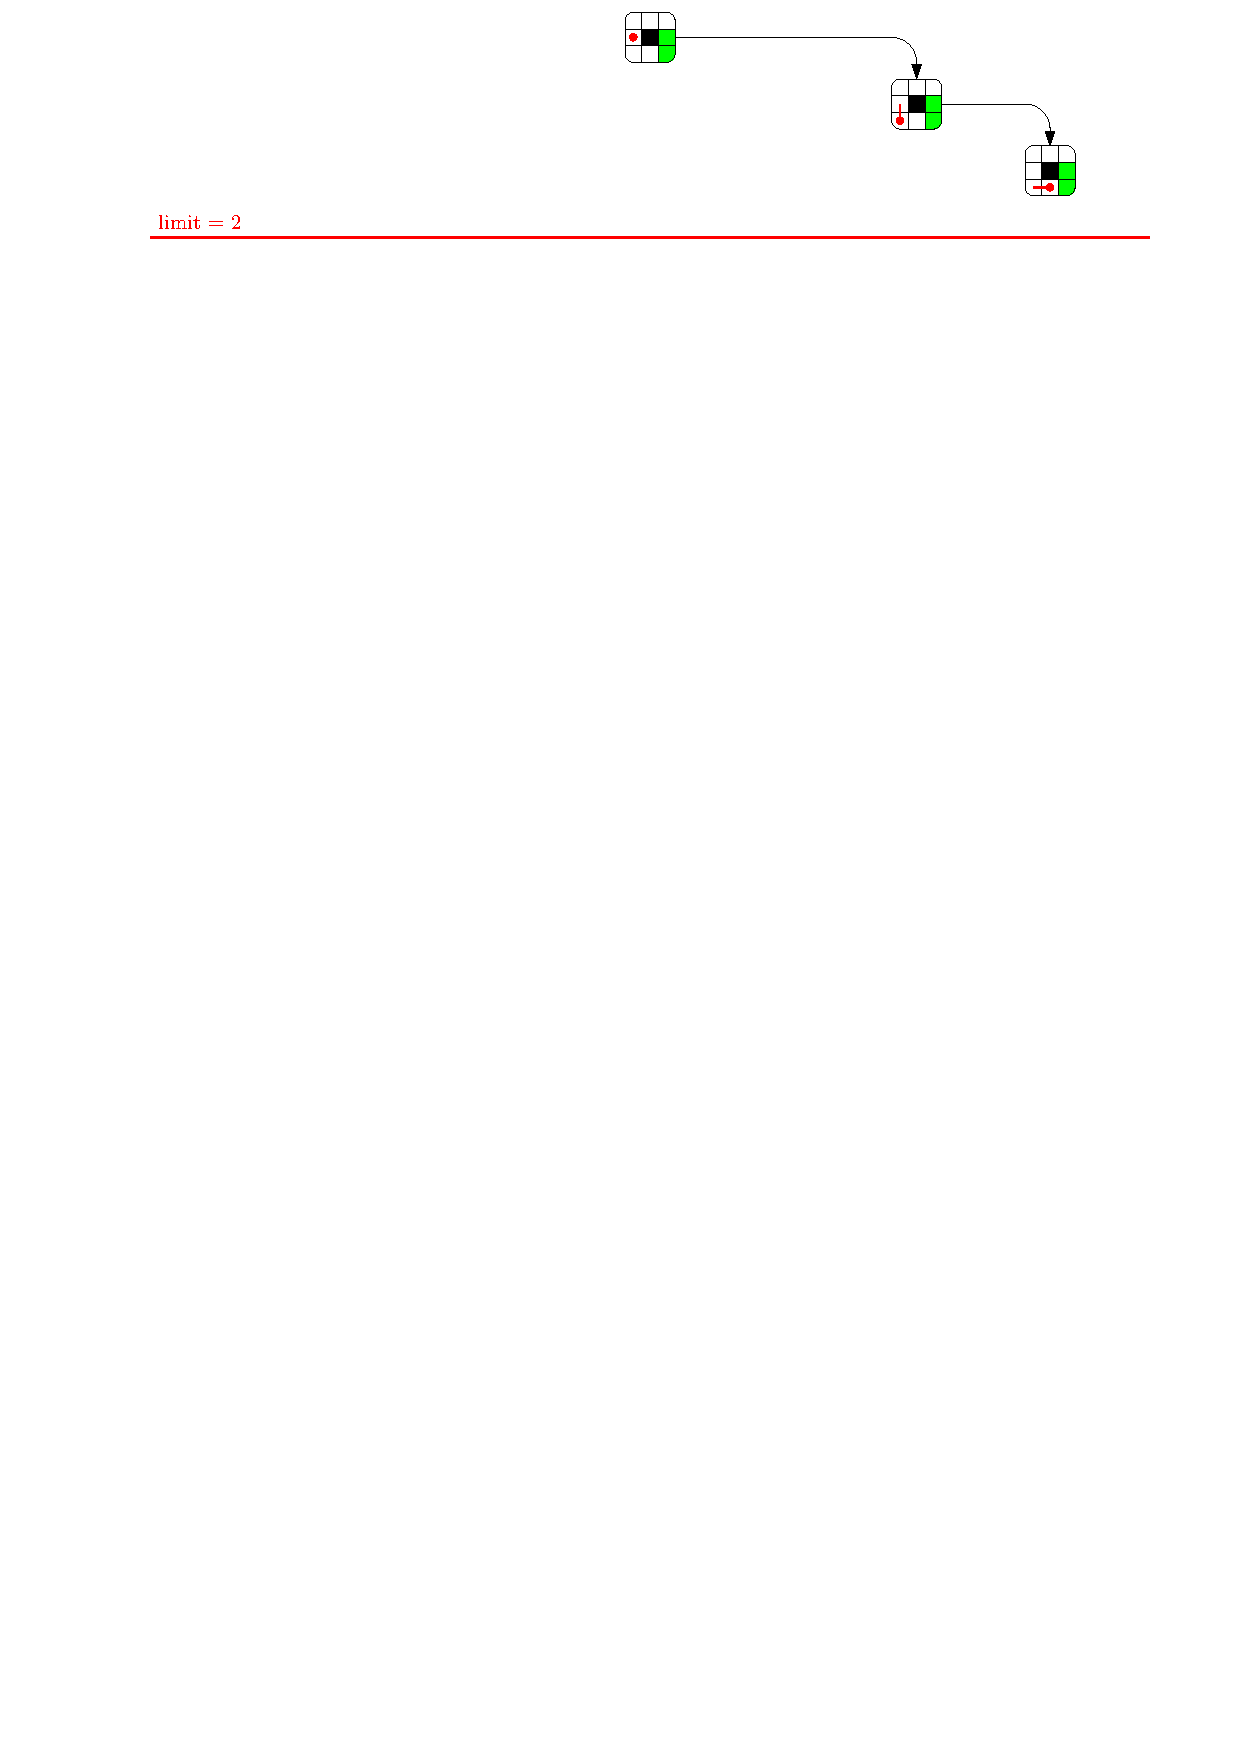
\includegraphics[width=\linewidth]{figs/iddfs16.pdf}}%
  \only<18>{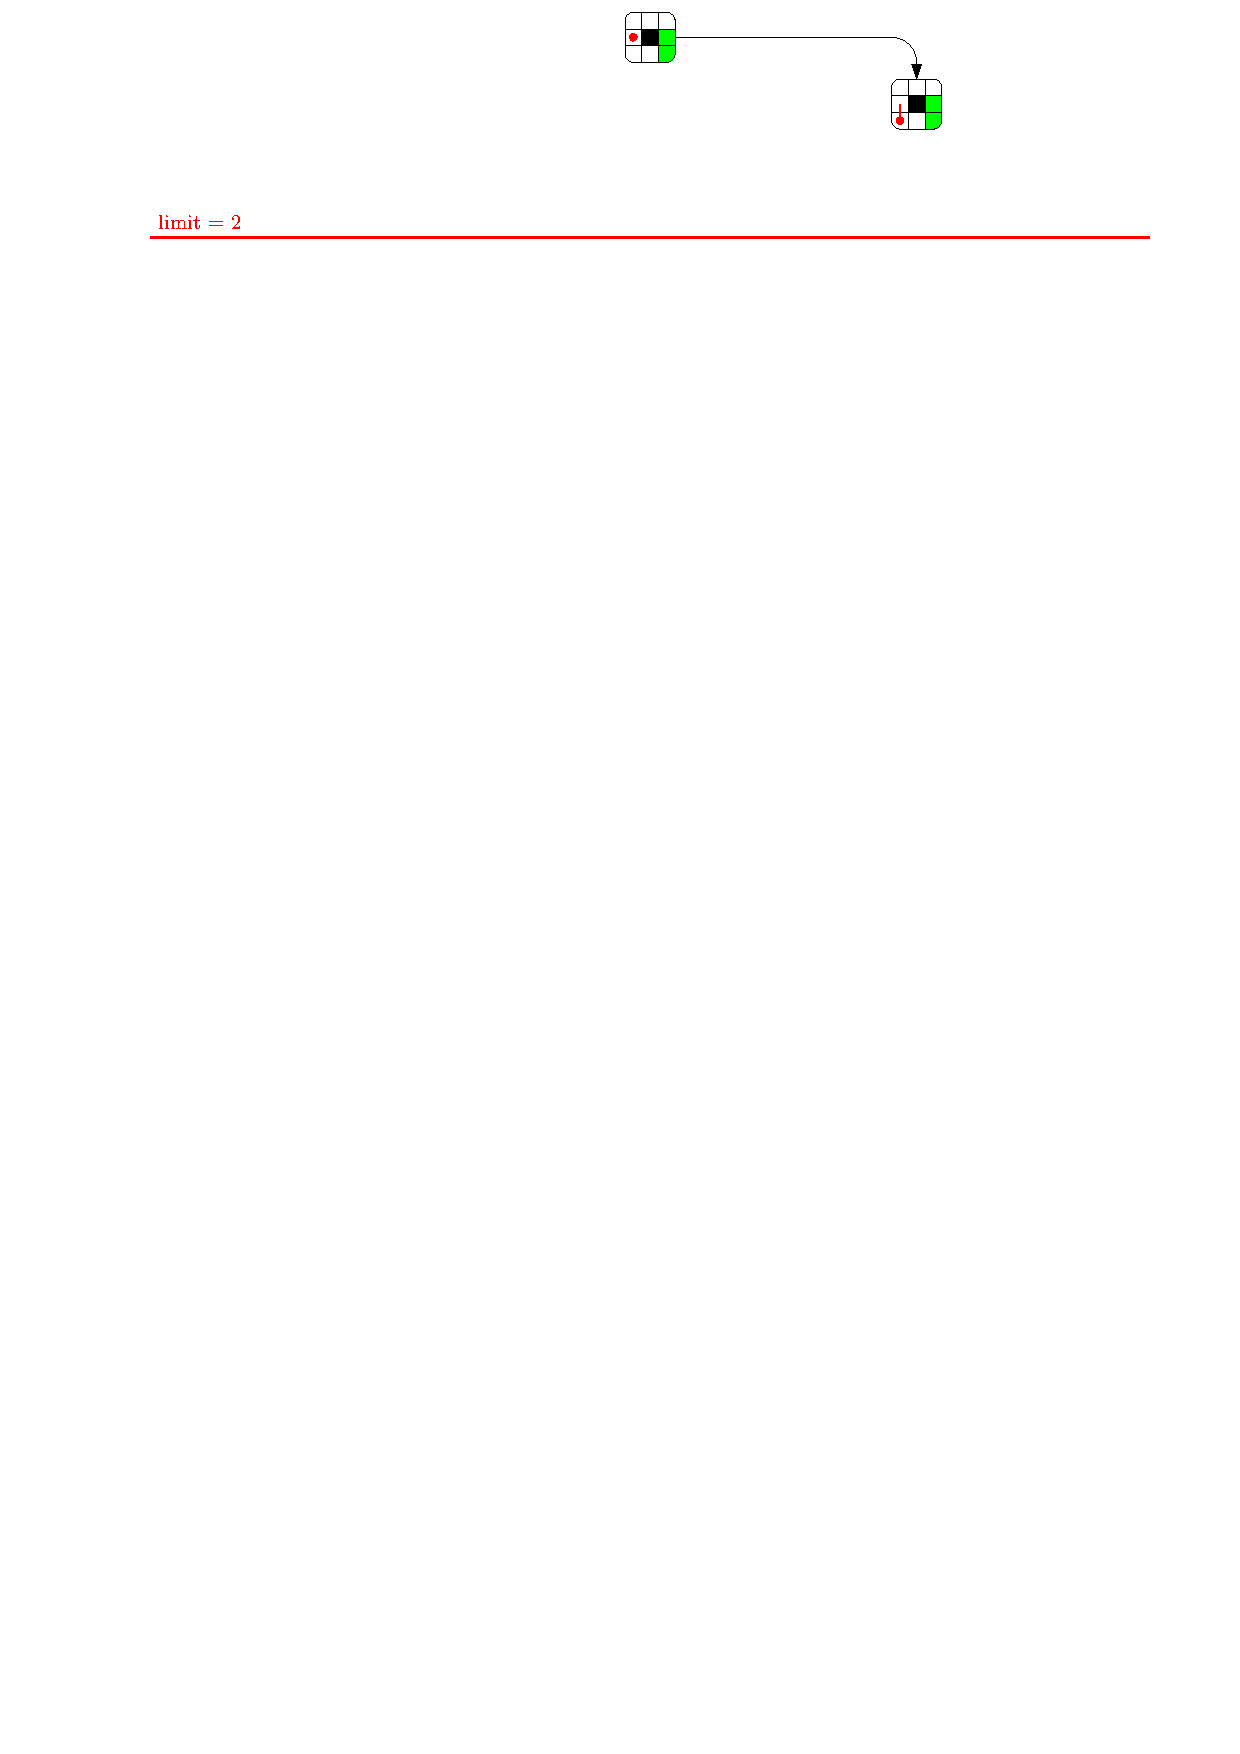
\includegraphics[width=\linewidth]{figs/iddfs18.pdf}}%
  \only<19>{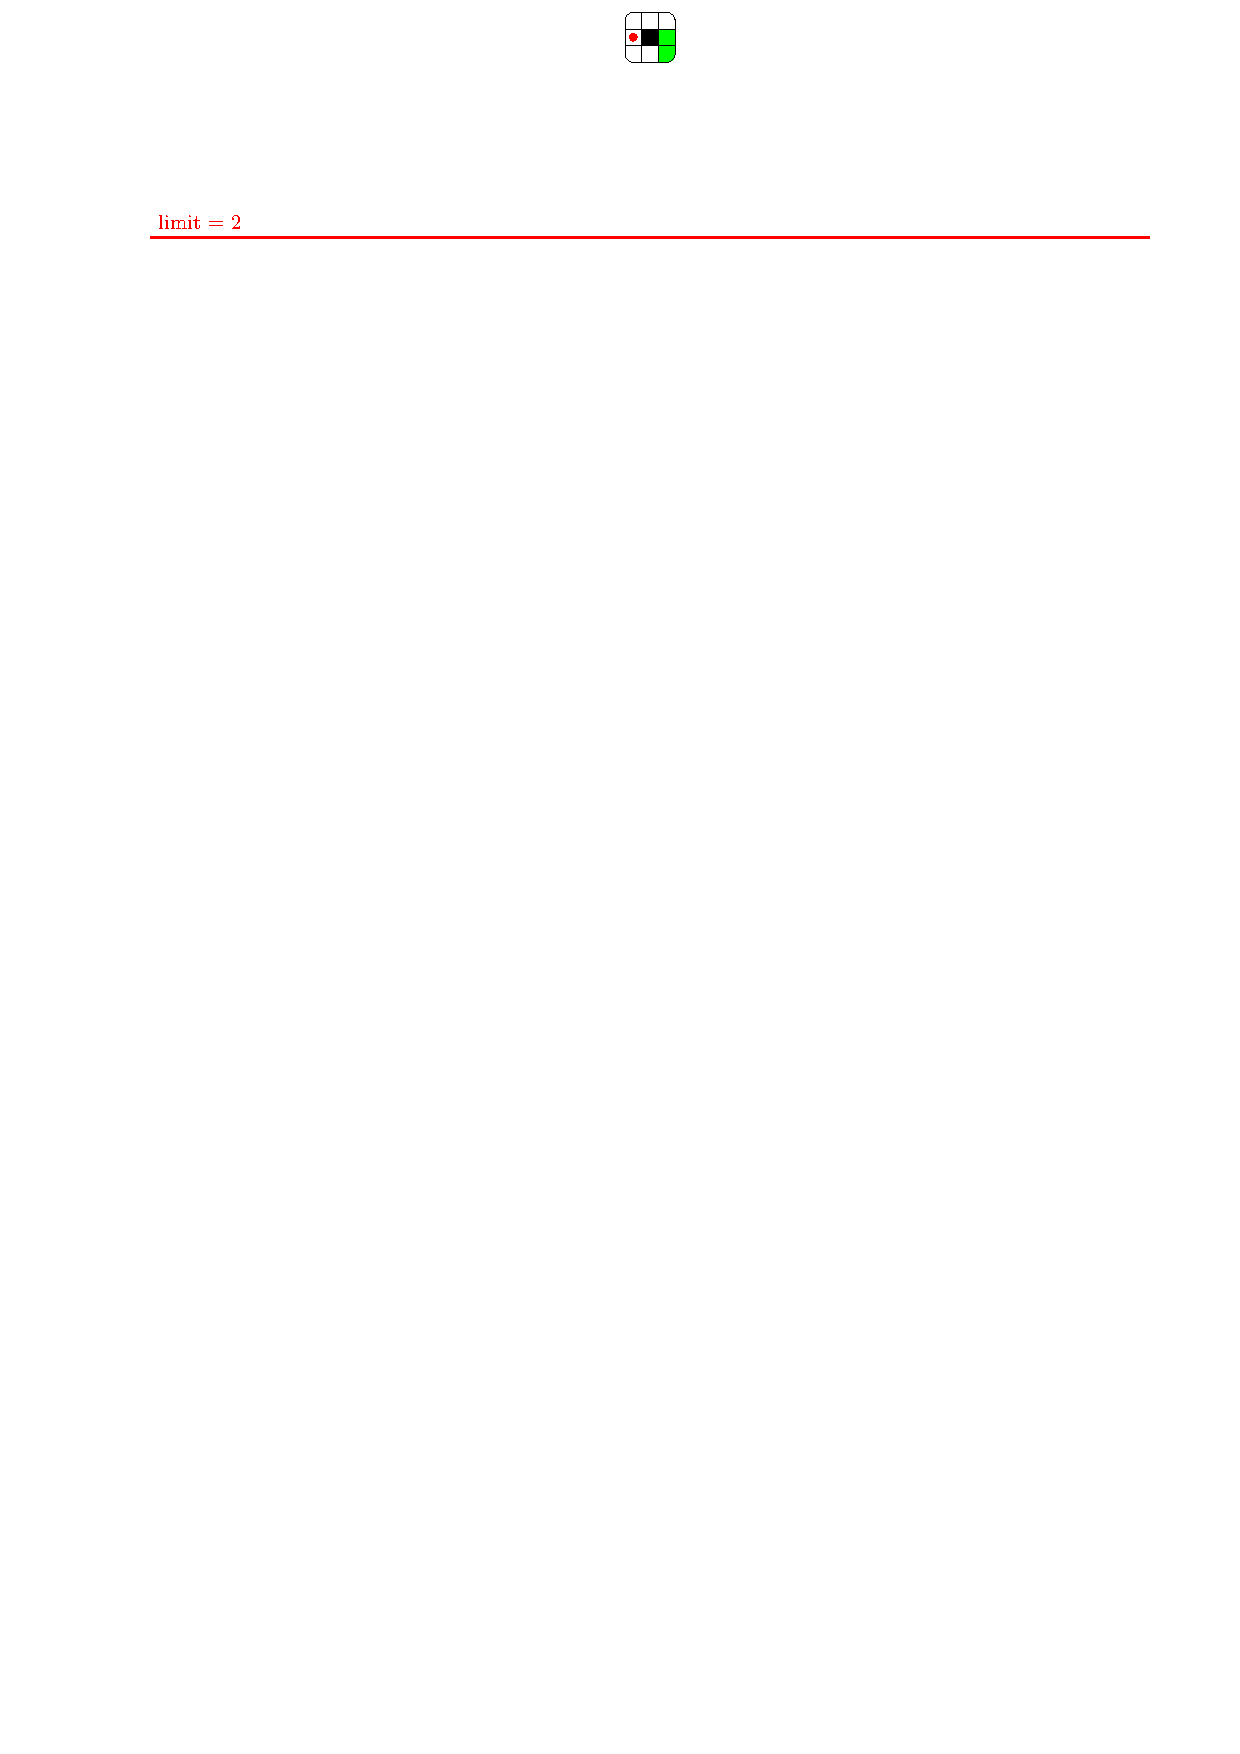
\includegraphics[width=\linewidth]{figs/iddfs22.pdf}}%
  \only<20>{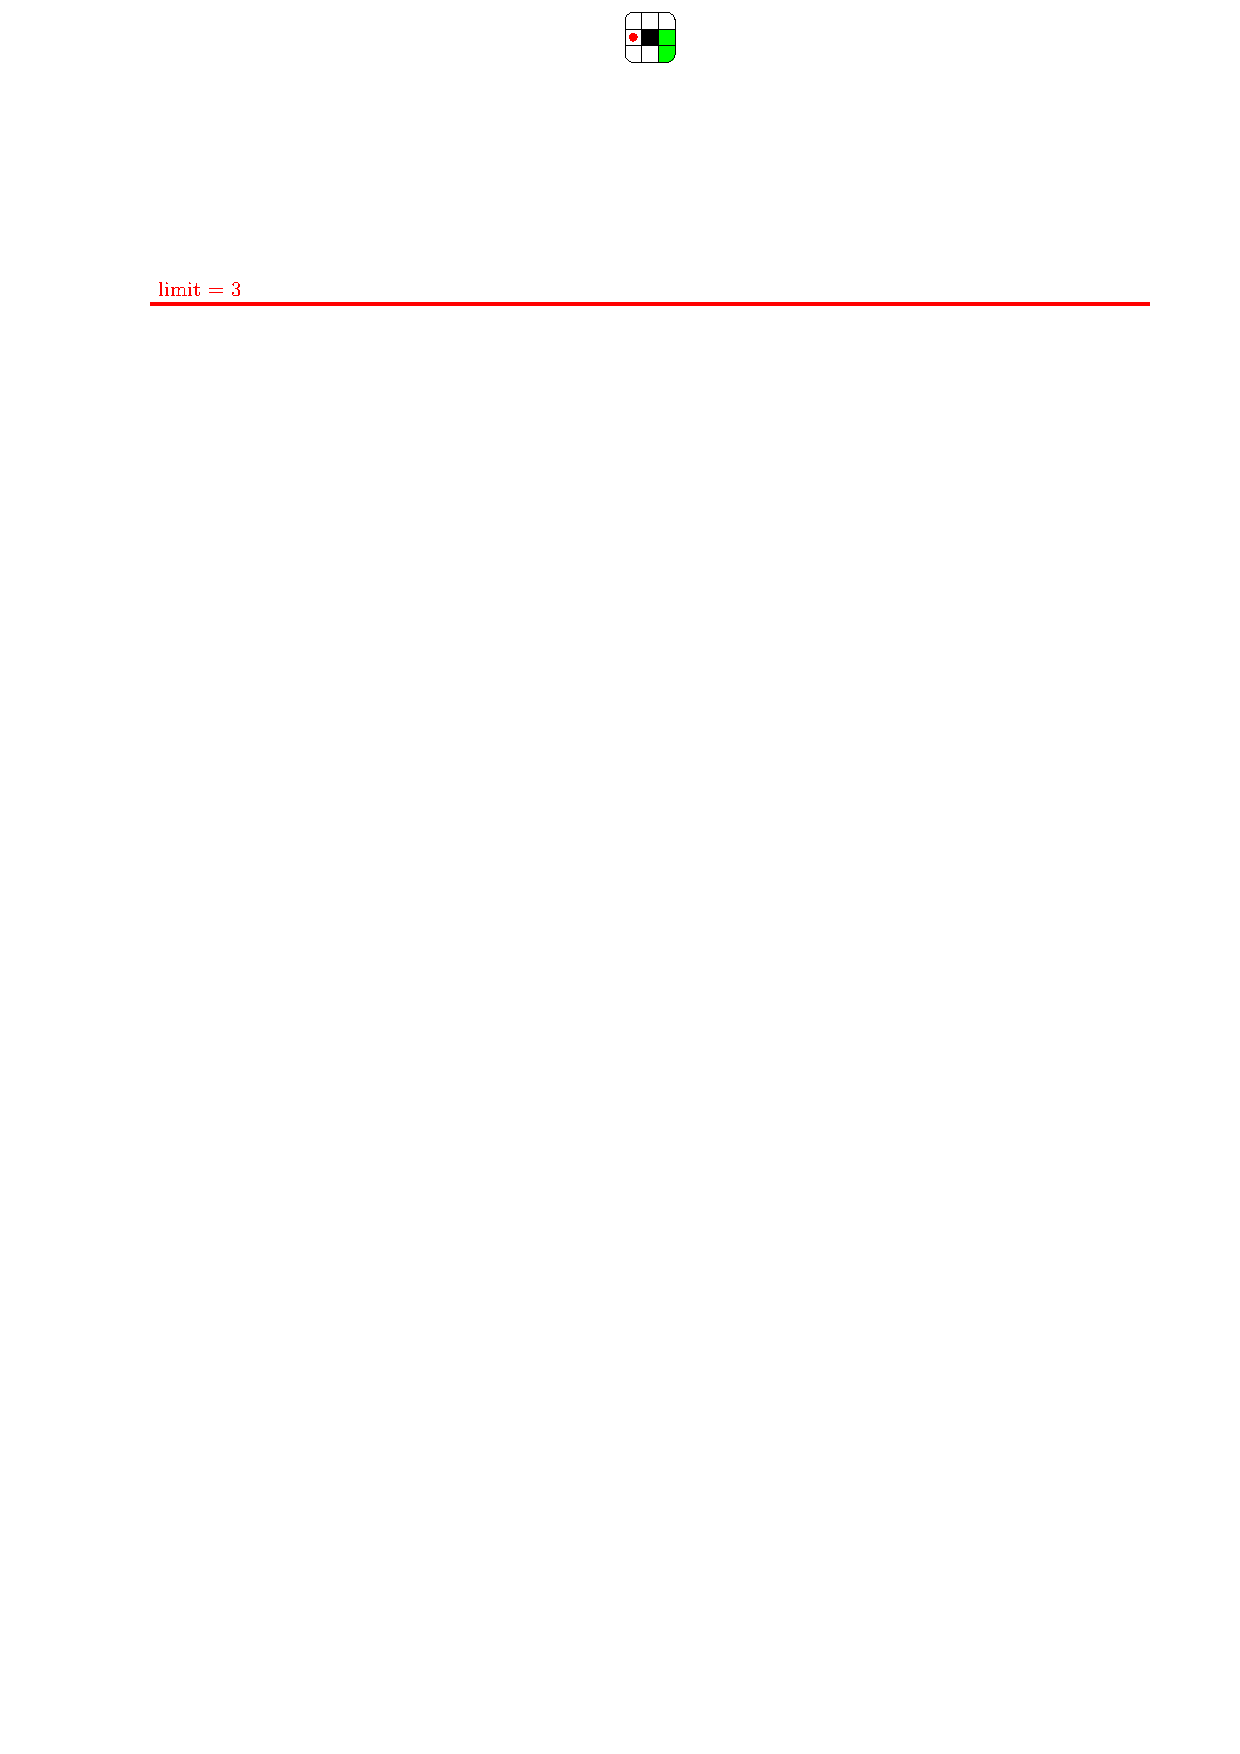
\includegraphics[width=\linewidth]{figs/iddfs15.pdf}}%
  \only<21>{\includegraphics[width=\linewidth]{figs/iddfs14.pdf}}%
  \only<22>{\includegraphics[width=\linewidth]{figs/iddfs13.pdf}}%
  \only<23>{\includegraphics[width=\linewidth]{figs/iddfs12.pdf}}%
  \only<24>{\includegraphics[width=\linewidth]{figs/iddfs13.pdf}}%
  \only<25>{\includegraphics[width=\linewidth]{figs/iddfs11.pdf}}%
  \only<26>{\includegraphics[width=\linewidth]{figs/iddfs13.pdf}}%
  \only<27>{\includegraphics[width=\linewidth]{figs/iddfs14.pdf}}%
  \only<28>{\includegraphics[width=\linewidth]{figs/iddfs10.pdf}}%
  \only<29>{\includegraphics[width=\linewidth]{figs/iddfs9.pdf}}%
  \only<30>{\includegraphics[width=\linewidth]{figs/iddfs10.pdf}}%
  \only<31>{\includegraphics[width=\linewidth]{figs/iddfs8.pdf}}%
  \only<32>{\includegraphics[width=\linewidth]{figs/iddfs10.pdf}}%
  \only<33>{\includegraphics[width=\linewidth]{figs/iddfs14.pdf}}%
  \only<34>{\includegraphics[width=\linewidth]{figs/iddfs15.pdf}}%
  \only<35>{\includegraphics[width=\linewidth]{figs/iddfs7.pdf}}%
  \only<36>{\includegraphics[width=\linewidth]{figs/iddfs6.pdf}}%
  \only<37>{\includegraphics[width=\linewidth]{figs/iddfs5.pdf}}%
  \only<38>{\includegraphics[width=\linewidth]{figs/iddfs6.pdf}}%
  \only<39>{\includegraphics[width=\linewidth]{figs/iddfs4.pdf}}%
  \only<40>{\includegraphics[width=\linewidth]{figs/iddfs6.pdf}}%
  \only<41>{\includegraphics[width=\linewidth]{figs/iddfs7.pdf}}%
  \only<42>{\includegraphics[width=\linewidth]{figs/iddfs3.pdf}}%
  \only<43>{\includegraphics[width=\linewidth]{figs/iddfs2.pdf}}%
  \only<44>{\includegraphics[width=\linewidth]{figs/iddfs3.pdf}}%
  \only<45->{\includegraphics[width=\linewidth]{figs/iddfs0.pdf}}%


  \vspace{1em}
  \only<46>{
    \begin{center}
      \Large V paměti máme pouze aktuální cestu :-)
    \end{center}
  }
\end{frame}

\begin{frame}
  Co byste ještě měli vylepšit?

  Nechceme vás příliš ovlivňovat...

  \vspace{1em}

  \begin{itemize}
  	\pause\item {\Large Některé uzly jsme navštěvovali mnohokrát (i na stejné cestě!)} \\
  	            (Zkuste zabránit vstupování do stejných stavů -- v paralelní verzi možná budete muset dělat kompromisy...) \\[0.7em]
  	\pause\item {\Large Nemusíte implementovat přesné verze těchto algoritmů}
  				(Například, v ID-DFS si můžete pamatovat o něco víc než jen aktuální cestu. Také můžete malé části stromu procházet pomocí BFS...)
  \end{itemize}

  \pause\vspace{1em}
  ... ale především po vás budeme chtít tyto algoritmy paralelizovat :-)
\end{frame}

\begin{frame}
  \frametitle{Shared pointers}

  {\Large Zejména v ID-DFS algoritmu je správná správa paměti nutností!} \\
  (Váš algoritmus musí být schopný běžet v prostředí s omezenou pamětí)

  \pause
  \vspace{1em}\hrule\vspace{1em}

  Dosud jste se pravděpodobně setkali zejména s \emph{raw pointery} ; \\
  napříkad \mintinline{c}{state * s;}

  \pause\vspace{1em}
  \hfill Veškerá zodpovědnost za správnou správu paměti by byla na vás :-(
\end{frame}

\begin{frame}
  \frametitle{Shared pointers}

  Naším cílem ale není zkoušet vás z toho, kdo je lepší programátor v C/C++...

  Proto správu paměti (částečně) přebíráme za vás!

  \hfill {\large Jak to děláme?}

  \pause\vspace{2em}

  \begin{center}
  	\Large\bf C++11 shared pointers
  \end{center}
\end{frame}

\begin{frame}[fragile]
  \frametitle{Shared pointers}

  S RAII návrhovým vzorem jsme se už setkali u \mintinline{c}{std::unique_lock}.

  \begin{minted}{c}
  template <typename lock_t>
  class unique_lock {
  private:
    lock_t & mutex;

  public:
    unique_lock(lock_t & mutex) : mutex(mutex) {
      mutex.lock();
    }

    ~unique_lock() {
      mutex.unlock();
    }
  };
  \end{minted}

  \pause
  \begin{center}
  	\Large Vlastnictví zámku je unikátní.
  \end{center}
\end{frame}

\begin{frame}[fragile]
  \frametitle{Shared pointers}

  Obdobně funguje i \texttt{std::unique\_ptr} pro správu pointeru.

  \hfill Paměť se uvolní okamžitě po zániku instance \texttt{std::unique\_ptr}!

  \vspace{0.5em}
  \begin{center}
  	\Large Co když to ale nechceme?
  \end{center}

  \vspace{2em}
  \begin{itemize}
  	\pause\item Instanci \texttt{std::unique\_ptr} uložíme například do vektoru.
  				Dále používáme raw pointer (získaný přes \texttt{ptr.get()}).

  				\hfill To ale na sebe opět bereme zodpovědnost za správu paměti! \\[0.3em]

  	\pause\item Důsledně budeme spravovat, kdo aktuálně pointer vlastní.
  				Paměť zanikne, když ho nějaká funkce nikomu nepředá (pomocí \texttt{std::move}).

  				\hfill To je celkem dost pracné! \\[0.3em]

  	\pause\item Použijeme \texttt{std::shared\_ptr} a pointery předáváme jako kdyby to byly raw pointery.
  \end{itemize}
\end{frame}

\begin{frame}
  \frametitle{Shared pointers}

  \textbf{Shared pointers} = jednoduchá automatická správa paměti (jednoduchý ,,garbage collector``)

  \begin{itemize}
  	\item Každý shared pointer si drží počítadlo, kolik instancí \texttt{std::shared\_ptr} na dané místo v paměti ukazuje
  	      \begin{itemize}
  	      	\item Při kopírování shared pointeru se počítadlo zvýší
  	      	\item Při rušení instance se počítadlo sníží
  	      \end{itemize}
  	\item Když počítadlo dospěje na nulu, paměť se dealokuje
  \end{itemize}
\end{frame}

\begin{frame}
  \frametitle{Shared pointers}

  Při rozumné práci fungují výborně, ale...

  \begin{center}
  	\LARGE \bf \faWarning \hspace{6pt} Pozor na cykly!!!
  \end{center}

  \vspace{1em}
  \begin{center}
  	\only<1>{\hfill\includegraphics[scale=0.9]{figs/sharedptr1.pdf}}%
  	\only<2>{\hfill\includegraphics[scale=0.9]{figs/sharedptr2.pdf}}%
  \end{center}
\end{frame}

\begin{frame}[fragile]
  \frametitle{Shared pointer}

  Se shared pointery dokonce můžete provádět atomické operace:
  \begin{minted}{c}
// 'atomicka promenna'
std::shared_ptr<const state> & concurrent_ptr = ...;

// ocekavana hodnota:
std::shared_ptr<const state> local_copy
                     = atomic_load(&concurrent_ptr);

// hodnota k zapsani
std::shared_ptr<const state> new_ptr = ...;

while(...) {
  if(atomic_compare_exchange_strong(
          &concurrent_ptr, &local_copy, new_ptr)) {
    break;
  }
}
  \end{minted}
\end{frame}

{\setbeamertemplate{frame footer}{\see{{\tt algorithms/iddfs.cpp} \sep {\tt make PDV\_Search}}}
\begin{frame}[fragile]
\frametitle{Sekvenční IDDFS}

  \begin{block}{Doimplementujte metodu \texttt{iddfs}}
    Doimplementujte tělo metody \texttt{iddfs}, která bude vykonávat sekvenční prohledávání do hloubky s definovanou maximální hloubkou (kterou budete iterativně zvyšovat, dokud nenarazíte na cíl). Vyzkoušejte si práci se sdílenými ukazateli a s doménovými metodami \texttt{is\_goal()} a \texttt{next\_states()}.
  \end{block}

\end{frame}
}

% Frame with the feedback QR code 
\framefeedback{}

\end{document}
